\documentclass[10pt,oneside]{book}
\usepackage{hyperref}
\usepackage{nameref}
\usepackage{minted}
\usepackage{graphicx}
\usepackage{enumitem}
\usepackage{calc}
\usepackage{tikz}
\usepackage[margin=1in]{geometry}
\usepackage[small,compact]{titlesec}
\usepackage[binary,squaren]{SIunits}
\usetikzlibrary{arrows}
\usetikzlibrary{decorations.markings}

\AtBeginDocument{\renewcommand{\bibname}{References}}

\newcommand{\hdhref}[2]{\href{#1}{#2}\footnote{\href{#1}{#1}}}
\newcommand{\funcdesc}{\vspace{-0.5\baselineskip}\noindent}
\newcommand{\funcsep}{\vspace{0.5\baselineskip}}
\newcommand{\HyperDexVersion}{1.0.dev}

% http://texblog.org/2012/03/21/cross-referencing-list-items/
\makeatletter
\def\namedlabel#1#2{\begingroup
    #2%
    \def\@currentlabel{#2}%
    \phantomsection\label{#1}\endgroup
}
\makeatother

\setcounter{secnumdepth}{3}
\setcounter{tocdepth}{3}

\title{HyperDex Reference Manual v1.0.dev}
\date{October 07, 2013}
\author{Robert Escriva, Bernard Wong, and Emin Gün Sirer}

\newminted{c}{samepage}
\newminted{console}{samepage}
\newminted{python}{samepage}

\begin{document}

\frontmatter
\maketitle
\tableofcontents

\mainmatter

\chapter{Introduction}

\section{Why HyperDex?}

HyperDex is the next-generation key-value store, designed from the ground up to
provide a convenient user interface without sacrificing reliability, robustness,
or performance.  First and foremost, HyperDex enables developers to create new
applications quickly and with strong correctness guarantees.
HyperDex features:

\begin{description}
\item[Performance:]  HyperDex achieves lower latency and higher throughput than
many other key-value stores.  Deploy fewer machines to support your application,
and save on operational costs.

\item[Consistency:]  HyperDex provides strongly-consistent reads, writes, and
atomic operations, making strong guarantees to your application.  Other
key-value stores promise \texttt{eventual} consistency, leaving your application
to pick up the slack.  HyperDex solves the tough problems, enabling you to write
correct applications quickly with less effort.

\item[Fault Tolerance:]  HyperDex employs a unique, built-in fault-tolerance
mechanism to safe-guard your data.  Simply tell HyperDex how many failures your
cluster is likely to experience, and HyperDex ensures that your data is
replicated to withstand at least that many failures.  Where other systems
require you to fully understand the replication internals to bring
fault-tolerance your data, HyperDex's fault-tolerance mechanism is simple to
understand and straightforward to use.

\item[Scalability:]  HyperDex automatically scales as more machines are added to
the system.  Add additional servers to your HyperDex cluster to increase storage
capacity and achievable throughput.

\item[Easy-to-Use:]  HyperDex is easy to use in both development and production
environments.  Set up a HyperDex cluster quickly, and scale out to multiple
machines without any application-level changes.  Other systems may require that
your application know about internals of the deployment, such as cluster
membership, replication options, and sharding configurations.  HyperDex
internally and automatically manages your cluster so your application doesn't
have to.
\end{description}

\section{About this Book}

This book is the definitive HyperDex reference manual for users, administrators,
and developers.  The HyperDex developers update this manual in tandem with each
release to ensure that the book serves as the best reference for HyperDex.

This book is divided into four parts, each of which is directed to a different
audience.  Part~\ref{part:for-developers}, ``For Developers'', provides an
introduction to HyperDex suitable for developers looking to build applications
on top of HyperDex.  The ``For Developers'' part of this book is written as a
series of tutorials that acquaint you with HyperDex's API and describe many of
the features available within HyperDex.

Part~\ref{part:for-admins}, ``For Administrators'', describes the day-to-day
maintenance of a HyperDex cluster.  The ``For Administrators'' portion of this
book is written as a series of small, isolated recipes that provide instruction
for maintaining and monitoring HyperDex clusters.

Part~\ref{part:for-hackers}, ``For Hackers'', should be of interest to
individuals looking to hack on HyperDex itself.  This portion of the book
provides pointers to enterprising individuals looking to extend, modify, or
contribute to HyperDex development.

Finally, Part~\ref{part:api-ref} provides an API reference for HyperDex.  This
section serves primarily as a reference of the developer-visible, and
operations-visible, components of HyperDex and should probably be used for
reference rather than read in its entirety.

This book is a continuous work in progress, and newer versions are available at
the \href{http://hyperdex.org/}{HyperDex website}.  The book's sources are
maintained alongside the HyperDex source code as the de-facto documentation for
HyperDex.  Patches, suggestions, and feedback about this book are welcome and
may be submitted using the contact information in the next section.

\section{Help and Support}

If you run into trouble while working with HyperDex, don't panic!  The HyperDex
team have put together many support avenues to assist you with HyperDex.  Many
of the available resources are freely available online.  When you need more
support than that, the HyperDex team is on standby with commercial support
options that ensure that you're never left in the dark.

\subsection{Online and Free Resources}

The HyperDex team have assembled several free online resources to help you make
the most of HyperDex:

\begin{itemize}
\item HyperDex Reference Manual:  This document is the best avenue for support
    and assistance.  It serves as the canonical documentation of HyperDex and
    should be your first stop with any questions or problems.
\item \href{https://groups.google.com/group/hyperdex-discuss}{HyperDex Mailing List}:
    This open mailing list is most users' first resource solving problems.
    Messages to the list are archived which makes it easy to search for
    solutions to your problem.  If you don't find a solution in the archives,
    start a new thread with your question and the HyperDex developers will try
    to help answer your questions.
\item \href{http://webchat.freenode.net/?channels=hyperdex\&uio=d4}{HyperDex IRC Channel}:
    The \texttt{\#hyperdex} IRC channel on Freenode is a great place to ask
    questions and interact with the HyperDex developers in real-time.
\item \href{https://github.com/rescrv/HyperDex/issues}{HyperDex Bug Tracker}:
    If you've encountered an error in the code that you think may be a bug,
    check the bug tracker to see if other users have reported the same problem.
    Consider reporting the problem yourself if it looks like the problem has not
    yet been reported.
\item \href{http://hyperdex.org/FAQ/}{HyperDex FAQ}:
    If you've got a question, check out the FAQ for frequently asked (and
    answered) questions.  The FAQ contains pointers to other resources to help
    solve your problems.
\item \href{http://hyperdex.org/papers/}{HyperDex Papers}:
    If you're interested in developing or changing the internals of HyperDex,
    we've published papers that detail the internal architecture and design
    principles of HyperDex.
\end{itemize}

\subsection{Commercial Support}

The HyperDex team provides commercial support for HyperDex, which includes
around-the-clock email support and consulting services.  If you're in need of
support, you can contact the HyperDex developers directly at {\em support}@{\em
hyperdex.org}.

\chapter{Installing HyperDex}
\label{chap:installation}

HyperDex provides multiple installation methods for a variety of environments.
Those looking to play around with HyperDex and go through the tutorials may find
it easiest to start with the quickstart Docker container.  For Linux users, the
easiest and most convenient way to install HyperDex is to use pre-compiled
binary packages.  OS X users have the option to install using Homebrew
packages.  Finally, HyperDex is also distributed as a set of tarballs so that
power users may install HyperDex in a custom manner on their platform of choice.

\section{Quick Installation with Docker}

HyperDex supports running within Docker containers for easy deployment.  With
Docker, an application is isolated in its own container, unable to change the
workstation outside the container.  This makes it easy to rapidly deploy new
applications without worrying about having to cleanup or revert any changes they
may make to the OS.  This sample environment is fully feature-complete, and
applications developed against such an environment will work with distributed
and sharded HyperDex clusters with zero application level changes.

For HyperDex, we can leverage containers to setup short-lived clusters that may
be used for one-off tasks, rapid prototyping, or for going through the HyperDex
tutorial---all without any commitment or modification to our base OS.  The
\code{hyperdex/quickstart} container includes everything necessary to run a
single-node HyperDex cluster, including the coordinator, daemon, and Python
bindings.

Running the HyperDex quickstart container is a simple three-step process:

\begin{enumerate}
\item We'll need Docker installed to use this container, which may be done by
following the \href{https://docs.docker.com/installation/}{Docker installation
instructions}.
\item We then fetch the HyperDex with the command \code{docker pull
hyperdex/quickstart}.
\item To start the cluster, run \code{docker run --net=host
-t -i hyperdex/quickstart}.  When all goes well, you'll see the following message
indicating your cluster is ready for use:

\begin{verbatim}
...
daemon: I1230 19:59:50.547586    21 daemon.cc:492] reconfiguration complete...
The transient HyperDex cluster is now online.

This is a transient HyperDex cluster.
You can connect to this cluster at address=172.17.3.27, port=1982.
\end{verbatim}
\end{enumerate}

With this quickstart cluster, both the coordinator and daemon logs will be
displayed on stdout.  You can connect to the cluster at the address and port
listed and can stop the cluster at any time using the command displayed on your
console.  When you stop the cluster, the HyperDex cluster will be destroyed, and
taken offline automatically.  To fully clean up any disk space in use by the
cluster, run \code{docker rm b6ae7c60c275}, where b6ae7c60c275 is the ID of your
quickstart container.

\section{Installing on CentOS/RedHat Using Binary Packages}

The following code snippet will install HyperDex on any 64-bit CentOS 6 or 7
system.  The script configures the HyperDex repository, imports the HyperDex
signing key, and installs the \code{hyperdex} package.  This script is available
in the HyperDex tarball or repository at \code{doc/install/centos-packages.sh}.

\inputminted[frame=lines,framesep=2mm,firstline=5]{bash}{\topdir/install/centos-packages.sh}

\noindent\textbf{Note:}  Users installing on Red Hat Enterprise Linux may have
to follow the instructions to install Extra Packages for Enterprise Linux
\footnote{\url{https://fedoraproject.org/wiki/EPEL}} prior to running the above
code.

\section{Installing on Debian Using Binary Packages}

The following code snippet will install HyperDex on any 64-bit Debian 7 (Wheezy)
system.  The script configures the HyperDex repository, imports the HyperDex
signing key, and installs the \code{HyperDex} package.  This script is available
in the HyperDex tarball or repository at \code{doc/install/debian7-packages.sh}.

\inputminted[frame=lines,framesep=2mm,firstline=5]{bash}{\topdir/install/debian7-packages.sh}

\section{Installing on Ubuntu Using Binary Packages}

The following code snippets will install HyperDex on 64-bit Ubuntu systems.
Pick the script that corresponds to the distribution you are running.  Each
script configures the HyperDex repository, imports the HyperDex signing key, and
installs the \code{HyperDex} package.  To figure out which version of Ubuntu you
are using, \code{cat /etc/os-release} and look for the corresponding version and
codename.

\subsection{Ubuntu 12.04 Precise Pangolin}

This script is available in the HyperDex tarball or repository at
\code{doc/install/ubuntu12.04-packages.sh}.

\inputminted[frame=lines,framesep=2mm,firstline=5]{bash}{\topdir/install/ubuntu12.04-packages.sh}

\subsection{Ubuntu 14.04 Trusty Tahr}

This script is available in the HyperDex tarball or repository at
\code{doc/install/ubuntu14.04-packages.sh}.

\inputminted[frame=lines,framesep=2mm,firstline=5]{bash}{\topdir/install/ubuntu14.04-packages.sh}

\section{Installing on Fedora Using Binary Packages}

The following code snippet will install HyperDex on any 64-bit Fedora 20 system.
The script configures the HyperDex repository, imports the HyperDex signing key,
and installs the \code{hyperdex} package.  This script is available in the
HyperDex tarball or repository at \code{doc/install/fedora-packages.sh}.

\inputminted[frame=lines,framesep=2mm,firstline=5]{bash}{\topdir/install/fedora-packages.sh}

\section{Installing on Linux Using Universal Binaries}
\label{sec:installation:universal-linux}

HyperDex is also available as a self-contained universal binary that works on
most glibc-based Linux distributions.  To use this installation, first download
the requisite tarball, and then you can install HyperDex like this:

\inputminted[frame=lines,framesep=2mm,firstline=3]{bash}{\topdir/install/linux-amd64.sh}

\section{Installing on OS X Using Homebrew}
\label{sec:installation:os-x-homebrew}

HyperDex is available on Mac OS X using the Homebrew package manager.  The
following script, available in the HyperDex tarball or repository at
\code{doc/install/homebrew.sh} may be used to install HyperDex on OS X:

\inputminted[frame=lines,framesep=2mm,firstline=3]{bash}{\topdir/install/homebrew.sh}

\section{Installing From Source}

Installing from source tarballs is a straightforward process that works on most
any recent Linux distribution.  Using the source tarballs provides power users
with control over the installation process and the opportunity to customize
the HyperDex installation.

To install from source, we must first prepare the system by installing a
compiler, and dependencies that are not managed by the HyperDex team.  This
process will be highly system specific, but should be familiar to most users who
install from source.  The HyperDex team and community are always happy to
provide assistance to users installing from source.

On systems like Ubuntu, we can prepare the system for the from-source install
with these commands:

\inputminted[frame=lines,framesep=2mm,firstline=3]{bash}{\topdir/install/ubuntu14.04-source-prereqs.sh}

With the prereqs installed, installing HyperDex from tarballs may be
accomplished with this script:

\inputminted[frame=lines,framesep=2mm,firstline=5]{bash}{\topdir/install/source-install.sh}

\subsubsection{Changing the Installation Directory}
\label{sec:installation:source:prefix}

By default, HyperDex installs files in \texttt{/usr/local}.  If you'd like to
install HyperDex elsewhere, you can specify the installation prefix at configure
time.  For example, to install HyperDex in \texttt{/opt/hyperdex}:

\begin{consolecode}
export PKG_CONFIG_PATH=/opt/hyperdex/lib/pkgconfig
./configure --prefix=/opt/hyperdex
\end{consolecode}

Check the \texttt{--help} option to configure for more ways to tune where
HyperDex places files.

%Dependencies for Python Bindings:
%
%\begin{itemize}
%\item \href{http://python.org/}{Python}: Version 2.6 or 2.7 with the
%    development headers installed.
%\end{itemize}
%
%Dependencies for Java Bindings:
%
%\begin{itemize}
%\item \href{http://openjdk.java.net/}{Java}: We test against OpenJDK 7.  Your
%    system must include \texttt{javac}, \texttt{jar}, and the JNI development
%    headers.
%\end{itemize}
%
%Dependencies for Yahoo! Cloud Serving Benchmark (YCSB):
%
%\begin{itemize}
%\item \href{https://github.com/brianfrankcooper/YCSB/wiki}{YCSB} The YCSB
%    distribution is a moving target.  We generally build against the latest Git
%    release.
%\end{itemize}
%
%\subsection{Configuring}
%\label{sec:installation:source:configure}
%
%HyperDex uses the Autotools to make configuration and installation as
%straightforward as possible.  After extracting the HyperDex tarball, you'll need
%to configure HyperDex.  The simplest configuration installs HyperDex in its
%default location (\texttt{/usr/local}) using the C++ compiler found on the
%system.  The configuration is performed in the directory extracted from the
%tarball and looks like:
%
%\begin{consolecode}
%./configure
%\end{consolecode}
%
%This basic configuration will configure the HyperDex daemon and native client
%library components to be built; however it omits several useful options for
%configuring HyperDex.  The rest of this section will highlight common ways to
%configure HyperDex.  Unless otherwise noted, all options should work well
%together.
%
%\subsubsection{Java Bindings}
%\label{sec:installation:source:java}
%
%HyperDex does not build Java bindings by default.  To enable the Java bindings,
%you must pass \texttt{--enable-java-bindings} to \texttt{./configure} like so:
%
%\begin{consolecode}
%./configure --enable-java-bindings
%\end{consolecode}
%
%If any of the prerequisites are missing \texttt{./configure} should fail.
%
%\begin{quote}
%Java bindings are currently unavailable in \HyperDexVersion.
%\end{quote}
%
%\subsubsection{Python Bindings}
%\label{sec:installation:source:python}
%
%HyperDex does not build Python bindings by default.  To enable the Python
%bindings, you must pass \texttt{--enable-python-bindings} to
%\texttt{./configure} like so:
%
%\begin{consolecode}
%./configure --enable-python-bindings
%\end{consolecode}
%
%If Python or its headers cannot be found, \texttt{./configure} will fail.
%
%\subsubsection{Yahoo! Cloud Serving Benchmark}
%\label{sec:installation:source:ycsb}
%
%HyperDex provides all the source code necessary to build a HyperDex driver
%for the YCSB benchmark.  If Java bindings are enabled, then YCSB can be built
%with \texttt{--enable-ycsb}.
%
%\begin{consolecode}
%./configure --enable-ycsb
%\end{consolecode}
%
%Note that YCSB must be in your Java \texttt{CLASSPATH}.  Configure cannot detect
%YCSB by itself.
%
%\section{Installing from Git}
%\label{sec:installation:git}
%
%Developers wishing to contribute to the development of HyperDex may build
%HyperDex directly from Git.  Building from Git is as straightforward as building
%from source tarballs, but requires a few extra dependencies and some setup
%before the \texttt{./configure} step.
%
%In order to build the HyperDex repository, you'll need to have the following
%utilities installed.  Most of these utilities are prepacked for Linux
%distributions.  Note that since these dependencies are only required for
%building from Git, they will not be detected at \texttt{./configure} time and
%instead \texttt{make} will fail with an error message.
%
%Required Dependencies:
%
%\begin{itemize}
%\item \href{http://www.gnu.org/software/autoconf/}{Autoconf} Used as part of
%    the build system.  Required for all builds.
%\item \href{http://www.gnu.org/software/automake/}{Automake} Used as part of
%    the build system.  Required for all builds.
%\item \href{http://www.gnu.org/software/libtool/}{Libtool} Used as part of the
%    build system.  Required for all builds.
%\item \href{http://www.gnu.org/software/autoconf-archive/}{Autoconf Archive}
%    Used as part of the build system.  Required for all builds.
%\item \href{http://www.freedesktop.org/wiki/Software/pkg-config/}{pkg-config}
%    Used as part of the build system.  Required for all builds.
%\item \href{http://flex.sourceforge.net/}{Flex} Used for building internal
%    parsers.  Required for all builds.
%\item \href{http://www.gnu.org/software/bison/}{Bison} Used for building
%    internal parsers.  Required for all builds.
%\item \href{http://cython.org/}{Cython} Used for building Python bindings.
%    Required for \texttt{--enable-python-bindings}.
%    Recommmended version: $\ge$ 0.15.
%\item \href{http://www.gnu.org/software/gperf/}{Gperf}  Generate perfect
%    hashes.  Used in the client library.
%\item \href{http://www.gnu.org/software/help2man/}{help2man}  Generate manual
%    pages with options.  Used for man-pages.
%\item \href{http://johnmacfarlane.net/pandoc/}{pandoc}  Convert manual pages
%    from markdown to man page format.
%\end{itemize}
%
%You'll need to build po6, e, BusyBee, HyperLevelDB Replicant, and HyperDex from
%Git, as the development version often introduces across repositories.
%
%For each of these repositories, you may build and install the code with:
%
%\begin{consolecode}
%autoreconf -i
%./configure
%make
%make install
%ldconfig
%\end{consolecode}

\subsection{Troubleshooting}
\label{sec:installation:troubleshooting}

This section walks through some common installation problems that might be
encountered while installing HyperDex from source.

\subsubsection{Missing \texttt{libtool}}
\label{sec:installation:troubleshooting:libtool}

If your system is missing \texttt{libtool}, you'll see an error message like the
following:

\begin{consolecode}
configure.ac:6: installing `./install-sh'
configure.ac:6: installing `./missing'
Makefile.am:48: Libtool library used but `LIBTOOL' is undefined
Makefile.am:48:   The usual way to define `LIBTOOL' is to add `LT_INIT'
Makefile.am:48:   to `configure.ac' and run `aclocal' and `autoconf' again.
Makefile.am:48:   If `LT_INIT' is in `configure.ac', make sure
Makefile.am:48:   its definition is in aclocal's search path.
Makefile.am: installing `./depcomp'
autoreconf: automake failed with exit status: 1
\end{consolecode}

To correct this issue, install the \code{libtool} package using your
distribution's package manager.

\subsubsection{Missing \texttt{pkgconfig}}
\label{sec:installation:troubleshooting:pkgconfig}

If your system is missing \texttt{pkgconfig}, you'll see an error message like
the following:

\begin{consolecode}
./configure: line 18348: syntax error near unexpected token `PO6,'
./configure: line 18348: `PKG_CHECK_MODULES(PO6, libpo6 >= 0.3.1)'
\end{consolecode}

To correct this issue, install the \code{pkg-config} package (sometimes called
\code{pkgconfig}) using your distribution's package manager.

\section{Verifying Installation}
\label{sec:installation:verify}

Once you have HyperDex installed, you should be able to view the built-in help.
If the following commands provide meaningful output, then it is very likely that
HyperDex is installed correctly and ready for use.

\begin{consolecode}
hyperdex help
hyperdex daemon --help
\end{consolecode}

\section{Upgrading to 1.6}
\label{sec:installation:upgrade1.6}

The 1.6 release introduces new features that are backwards incompatible with
previous releases, most notably a binary document format.  Before upgrading to
1.6, backup your data.  Once 1.6 is installed, copy your data into a
newly-deployed 1.6 cluster.

\section{Upgrading to 1.5}
\label{sec:installation:upgrade1.5}

HyperDex 1.5 is backwards compatible with the 1.4 on-disk format.  To upgrade
from 1.4 to 1.5, take a backup and restart the cluster from the backup.

\section{Upgrading to 1.4}
\label{sec:installation:upgrade1.4}

Upgrading to 1.4 is a two step process.  First, take a full backup of your
cluster using the provided backup tools.  Start the 1.4 cluster from the
backup.  This will upgrade the coordinator to 1.4, and the daemons will work
with the old data directory.

Alternatively take a backup, and restart the coordinator from the backed-up
coordinator state on the same address.  Then do a rolling restart of the
daemons.

The 1.4 release's on-disk format is backwards incompatible with the 1.3 and
prior releases.  HyperDex daemons will automatically upgrade to the 1.4 format
when first launched.

\section{Upgrading to 1.3}
\label{sec:installation:upgrade1.3}

Upgrading to 1.3 is a two step process.  First, take a full backup of your
cluster using the provided backup tools.  Start the 1.3 cluster from the
backup.  This will upgrade the coordinator to 1.3, and the daemons will work
with the old data directory.

Alternatively take a backup, and restart the coordinator from the backed-up
coordinator state on the same address.  Then do a rolling restart of the
daemons.

\section{Upgrading to 1.2}
\label{sec:installation:upgrade1.2}

The 1.2 release introduces new features that are backwards incompatible with
previous releases.  Before upgrading to 1.2, backup your data.  Once 1.2 is
installed, copy your data into a newly-deployed 1.2 cluster.


\part{For Developers}
\label{part:for-developers}
\chapter{Quick Start}
\label{chap:quick-start}

This chapter is designed to give you a whirlwind tour of HyperDex.  The first
section gives a high-level overview of a typical HyperDex deployment and
application.  Subsequent sections provide step-by-step instructions for how
HyperDex could be used to build store data for a hypothetical phone book
application.

\section{High-Level Overview}
\label{sec:quick-start:overview}

A HyperDex cluster consists of three types of components: clients, servers, and
coordinators.

Applications built on top of HyperDex are referred to as {\em clients}.  and
access HyperDex through various bindings for popular languages (e.g. C, C++,
Java, and Python) to issue operations such as \code{get}, \code{put},
\code{search}, \code{delete}, etc.

The HyperDex servers are responsible for storing the data in the system. You can
have a cluster with as few as just a single server, though typical installations
will have dozens to hundreds of servers. These servers store the data in memory
and on disk, and they can crash at any time. HyperDex can be configured to
tolerate as many failed nodes as desired.

The HyperDex coordinator maintains the entire cluster.  This involves making
sure that servers are up, as well as detecting, removing, and replacing failed
or slow nodes.  The coordinator maintains a critical data structure, the
hyperspace map, that establishes the mapping of data to servers.  Clients use
this map to locate the servers they need to contact, while servers use it to
perform object propagation and replication to achieve the application's desired
goals.

In this tutorial, we'll discuss how to get a HyperDex cluster up and running. In
particular, we'll create a simple space, insert objects into it, retrieve those
objects, and then perform queries over these objects.

\section{Starting the Coordinator}
\label{sec:quick-start:coordinator}

First, we need to start up a coordinator that will oversee the organization of
the hyperspace.

The following command starts and initializes the coordinator:

\begin{consolecode}
hyperdex coordinator -f -l 127.0.0.1 -p 1982
\end{consolecode}

The ``coordinator'' command spawns a new HyperDex coordinator process listening
on on the specified address.  All other servers are introduced to the HyperDex
cluster via this address, so it is important that it be accessible to all
servers.  For the purposes of this tutorial, binding to the loopback address
will suffice, but you will probably want to use a public IP address for a real
deployment

At this point, the coordinator is up and running, and we're ready to start up
additional nodes in our cluster.

\section{Starting HyperDex Daemons}
\label{sec:quick-start:daemon}

The HyperDex daemons are the workhorse processes that actually house the data in
the data store and respond to client requests. Let's start a daemon on the the
same machine as the coordinator by running this in another terminal window:

\begin{consolecode}
hyperdex daemon -f --listen=127.0.0.1 --listen-port=2012 \
                   --coordinator=127.0.0.1 --coordinator-port=1982 --data=/path/to/data
\end{consolecode}

This command runs HyperDex in the foreground, listens for incoming connections
on address 127.0.0.1:2012 and connects to the coordinator that we started
earlier.  This enables the daemon to announce its presence, which in turn
enables the coordinator to assign partitions of data to the newly arrived
daemon.  For example, the coordinator can direct the daemon to take over some of
the partitions from an existing daemon, participate in the data replication
protocol, and start handling client requests.  But since we have no data yet and
this is our first node, this particular daemons does not have much work to do.

Note that the second argument (127.0.0.1) is the IP address to which we want to
bind the daemon.  Once again, we are using a loopback address here for the
purposes of the tutorial, while in real life you will undoubtedly want to use
one of the IP addresses bound to your internal network.  If no address is
specified, HyperDex will attempt to autodetect an external address.

The last argument is a pointer to a directory where the daemon will store all
data.  Each HyperDex daemon must have its own data directory.

It doesn't hurt to start a few more daemon instances at this point (although it
is not required to continue with the tutorial).

You now have a functional HyperDex cluster.  It's time to do something with it.

\section{Creating a new Space}
\label{sec:quick-start:space}

Let's imagine that we are building a phone book application.  Such a phonebook
would end up keeping track of people's first name, last name, and phone number.
And to distinguish unique users, it might assign a user id to each user.  In
HyperDex, each such collection of data is called a {\em space} and is
conceptually similar to {\em tables} in traditional databases.  Let's see how we
can instruct HyperDex to create a suitable space for holding such objects.

First, let's open a Python shell and connect to HyperDex via the Admin interface:

\begin{pythoncode}
>>> import hyperdex.admin
>>> a = hyperdex.admin.Admin('127.0.0.1', 1982)
\end{pythoncode}

This line instructs the admin bindings to talk to the coordinator and get the
current cluster configuration.  There is no need for static configuration files.
Clients always receive the most up-to-date configuration, and if the
configuration changes, say, due to failures, the coordinator will detect that a
client is operating with an out-of-date configuration and instruct it to retry
with a fresh config.  The only thing a client must know to connect to a cluster
is the address of the cluster coordinator.

Let's programmatically create a new space using the Python bindings:

\begin{pythoncode}
>>> a.add_space('''
... space phonebook
... key username
... attributes first, last, int phone
... subspace first, last, phone
... create 8 partitions
... tolerate 2 failures
... ''')
True
\end{pythoncode}

This command creates a new space called ``phonebook'' that has a key of
``username'', and has attributes ``first'', ``last'', and ``phone''.  By
default, HyperDex treats every attribute as an opaque bytestring, but provides
other types as well.  Here, we specify that the phone number be treated as an
integer.  The available datatypes are discussed in
Chapter~\ref{chap:data-types}.

Even though the objects we specify will have many attributes, HyperDex will not
necessarily create one giant hyperdimensional space spanning as many dimensions
as attributes.  Doing so would not be desirable, as the space would be to large
to efficiently map onto a cluster.  Instead, we will typically want to create
{\em subspaces} consisting of smaller numbers of dimensions. The lower number of
dimensions enable the mapping from points in space to nodes in the cluster to be
more efficient; in particular, fewer nodes need to be contacted during search
operations.  In this simple example, we create a 3-dimensional subspace for the
{\em first}, {\em last} and {\em phone} attributes.  HyperDex always implicitly
creates a 1-dimensional subspace for the key of objects.

In other NoSQL systems, objects can {\em only} be retrieved efficiently by the
key under which they were inserted.  So an object <jsmith, John, Smith,
555-1234> can only be retrieved by its key ``jsmith''.  Subspaces enable
HyperDex to retrieve all ``John'' or ``Smith'' objects or, even, reverse lookups
by phone number.  The key serves as an object identifier so that objects may be
retrieved or stored efficiently.  Internally, the key is used to sequence
updates and ensure consistency.

Even though we've only deployed one server in this example, we may want to leave
room for future growth of our HyperDex cluster.  The ``create 8 partitions''
line specifies that HyperDex will partition the resulting space into 8 regions.
As a general rule, the number of partitions should be greater than the number of
daemons that will ever join the cluster.  It's perfectly acceptable to omit this
line, and HyperDex will partition the cluster into 256 regions.

Since large scale cloud-computing deployments are sure to encounter failures, we
will want to safeguard the data in our key-value store by replicating for fault
tolerance.  The ``phonebook'' space is configured to tolerate up to two
concurrent failures (``tolerate 2 failures'').  This instructs HyperDex to
protect against up to two failures by creating three replicas of each object.
Even if two daemons holding an object fail, there will still be one copy of the
object remaining.  HyperDex automatically repairs from this one remaining copy.

Finally, it's possible to create spaces using the command-line tools that ship
with HyperDex.  One could have created the ``phonebook'' space using the
command-line:

\begin{consolecode}
hyperdex add-space -h 127.0.0.1 -p 1982 << EOF
   space phonebook
   key username
   attributes first, last, int phone
   subspace first, last, phone
   create 8 partitions
   tolerate 2 failures
EOF
\end{consolecode}

\section{Interacting with the ``phonebook'' Space}
\label{sec:quick-start:phonebook}

Now that we have our hyperspace defined and ready to go, it's time to insert
some information into our phonebook.

Continuing in the same Python session, lets open a new Client connection to the
cluster.  HyperDex separates the metadata manipulation provided by the Admin
library from the data manipulation provided by the Client library.

\begin{pythoncode}
>>> import hyperdex.client
>>> c = hyperdex.client.Client('127.0.0.1', 1982)
\end{pythoncode}

We can create an object by doing the following:

\begin{pythoncode}
>>> c.put('phonebook', 'jsmith1', {'first': 'John', 'last': 'Smith',
...                                'phone': 6075551024})
True
\end{pythoncode}

This operation will determine the right spot in the hyperspace for this object
and issue the \code{put} operation to all replicas.  The operation will only
return once the object has been committed at all requisite nodes.

We can easily retrieve the same ``jsmith'' object by using a standard
\code{get}.

\begin{pythoncode}
>>> c.get('phonebook', 'jsmith1')
{'first': 'John', 'last': 'Smith', 'phone': 6075551024}
\end{pythoncode}

Yay!  We inserted an object under the key ``jsmith1'' and retrieved it using the
same key.  This looks exactly like every other NoSQL store out there, but there
are a few differences.

First, it's blazingly fast. You can look at our latest performance graphs for
the precise comparisons, but typically, HyperDex is just way faster than other
key-value stores.

Second, it's fault-tolerant. When we performed the \code{put}, our operation was
sent through a {\em value-dependent chain} of daemons assigned to the object.
The client received an acknowledgment only when the object was replicated on
every single server in the chain.  Unlike NoSQL stores that optimistically
assume that an update was committed before reaching all servers, HyperDex
responds only when all daemons have been updated.  And we can pick the
replication level to achieve any level of fault tolerance we desire.

Finally, it's consistent. If we had multiple concurrent \code{put} operations
being issued by multiple clients at the same time, we would never see an
inconsistent state.  What is an inconsistent state?  It's what you get when you
settle for {\em eventual consistency}.  For instance, we would not want a
prescription tracking system to say that we dispensed a drug, then to say we did
not, only to settle on (say) having dispensed it. Yet this is precisely what
might happen with an eventually consistent NoSQL key-value store.  Eventual
consistency is no consistency at all.  In contrast, HyperDex provides
linearizability. Time will never roll backwards from the point of any client.

And it gets better. Not only can we retrieve objects by their key, but we can
also retrieve them when we don't know their key. Here are some examples:

\begin{pythoncode}
>>> [x for x in c.search('phonebook', {'first': 'John'})]
[{'first': 'John',
  'last': 'Smith',
  'phone': 6075551024,
  'username': 'jsmith1'}]
>>> [x for x in c.search('phonebook', {'last': 'Smith'})]
[{'first': 'John',
  'last': 'Smith',
  'phone': 6075551024,
  'username': 'jsmith1'}]
\end{pythoncode}

Let's do that reverse phone number search:

\begin{pythoncode}
>>> [x for x in c.search('phonebook', {'phone': 6075551024})]
[{'first': 'John',
  'last': 'Smith',
  'phone': 6075551024,
  'username': 'jsmith1'}]
\end{pythoncode}

Here's a fully-qualified search. Hyperspace hashing makes this nearly as fast as
a key-based lookup:

\begin{pythoncode}
>>> [x for x in c.search('phonebook',
...  {'first': 'John', 'last': 'Smith', 'phone': 6075551024})]
[{'first': 'John',
  'last': 'Smith',
  'phone': 6075551024,
  'username': 'jsmith1'}]
\end{pythoncode}

Let's add another user named ``John Doe'':

\begin{pythoncode}
>>> c.put('phonebook', 'jd', {'first': 'John', 'last': 'Doe', 'phone': 6075557878})
True
>>> [x for x in c.search('phonebook',
...  {'first': 'John', 'last': 'Smith', 'phone': 6075551024})]
[{'first': 'John',
  'last': 'Smith',
  'phone': 6075551024,
  'username': 'jsmith1'}]
>>> [x for x in c.search('phonebook', {'first': 'John'})]
[{'first': 'John',
  'last': 'Smith',
  'phone': 6075551024,
  'username': 'jsmith1'},
 {'first': 'John',
  'last': 'Doe',
  'phone': 6075557878,
  'username': 'jd'}]
>>> [x for x in c.search('phonebook', {'last': 'Smith'})]
[{'first': 'John',
  'last': 'Smith',
  'phone': 6075551024,
  'username': 'jsmith1'}]
>>> [x for x in c.search('phonebook', {'last': 'Doe'})]
[{'first': 'John',
  'last': 'Doe',
  'phone': 6075557878,
  'username': 'jd'}]
\end{pythoncode}

Should John Doe decide he no longer wants to be listed in the phonebook, it's
trivial to remove his listing:

\begin{pythoncode}
>>> c.delete('phonebook', 'jd')
True
>>> [x for x in c.search('phonebook', {'first': 'John'})]
[{'first': 'John',
  'last': 'Smith',
  'phone': 6075551024,
  'username': 'jsmith1'}]
\end{pythoncode}

Suppose John Smith needs to change his phone number. This is easily accomplished
by specifying just the key for the object and the changed attribute.  All other
attributes will be preserved.

\begin{pythoncode}
>>> c.put('phonebook', 'jsmith1', {'phone': 6075552048})
True
>>> c.get('phonebook', 'jsmith1')
{'first': 'John',
  'last': 'Smith',
  'phone': 6075552048}
\end{pythoncode}

Smith is a popular name.  Let's say there was ``John Smith'' from Rochester
(area code 585):

\begin{pythoncode}
>>> c.put('phonebook', 'jsmith2',
...          {'first': 'John', 'last': 'Smith', 'phone': 5855552048})
True
>>> c.get('phonebook', 'jsmith2')
{'first': 'John',
  'last': 'Smith',
  'phone': 5855552048}
\end{pythoncode}

Suppose we want to locate everyone named ``John Smith'' from Ithaca (area code
607). We can do this with a range query in HyperDex.

\begin{pythoncode}
   >>> [x for x in c.search('phonebook',
   ...  {'last': 'Smith', 'phone': (6070000000, 6080000000)})]
   [{'first': 'John',
     'last': 'Smith',
     'phone': 6075552048,
     'username': 'jsmith1'}]
\end{pythoncode}

Or perhaps we want to search for everyone whose name falls between ``'Jack'``
and ``'Joseph'``:

\begin{pythoncode}
>>> [x for x in c.search('phonebook',
...  {'first': ('Jack', 'Joseph')})]
[{'first': 'John',
  'last': 'Smith',
  'phone': 6075552048,
  'username': 'jsmith1'},
 {'first': 'John',
  'last': 'Smith',
  'phone': 5855552048,
  'username': 'jsmith2'}]
\end{pythoncode}

\section{Cleaning Up}
\label{sec:quick-start:cleanup}

When we're done with the ``phonebook'' space, we can delete the space and all
the items in it directly from Python:

\begin{pythoncode}
>>> a.rm_space('phonebook')
True
\end{pythoncode}

\chapter{Data Types}
\label{chap:data-types}

As we saw in the previous chapter, HyperDex offers support for the basic
\code{get}, \code{put}, and \code{search} operations on strings and integers.
In this chapter, we explore HyperDex's richer datatypes and atomic operations on
lists, sets, and maps.  We will see how providing efficient atomic operations on
these rich, native datastructures greatly simplifies design for applications
with complicated data layout requirements.

By the end of this chapter you'll be familiar with all datatypes provided by
HyperDex, and a number of atomic operations.

\section{Setup}
\label{sec:data-types:setup}

As in the previous chapter, the first step is to deploy the cluster and connect
a client.   First we launch and initialize the coordinator:

\begin{consolecode}
hyperdex coordinator -f -l 127.0.0.1 -p 1982
\end{consolecode}

Next, let's launch a few daemon processes to store data.  Execute the following
commands (note that each instance binds to a different port and has a different
\code{/path/to/data}):

\begin{consolecode}
hyperdex daemon -f --listen=127.0.0.1 --listen-port=2012 \
                   --coordinator=127.0.0.1 --coordinator-port=1982 --data=/path/to/data1
hyperdex daemon -f --listen=127.0.0.1 --listen-port=2013 \
                   --coordinator=127.0.0.1 --coordinator-port=1982 --data=/path/to/data2
hyperdex daemon -f --listen=127.0.0.1 --listen-port=2014 \
                   --coordinator=127.0.0.1 --coordinator-port=1982 --data=/path/to/data3
\end{consolecode}

This brings up three different daemons ready to serve in the HyperDex cluster.
Finally, we create a space which makes use of all three systems in the cluster.
In this example, let's create a space that may be suitable for storing profiles
in a social network:

\begin{pythoncode}
>>> import hyperdex.admin
>>> a = hyperdex.admin.Admin('127.0.0.1', 1982)
>>> a.add_space('''
... space profiles
... key username
... attributes
...    string first,
...    string last,
...    int profile_views,
...    list(string) pending_requests,
...    set(string) hobbies,
...    map(string, string) unread_messages,
...    map(string, int) upvotes
... subspace first, last
... subspace profile_views
... ''')
True
>>> import hyperdex.client
>>> c = hyperdex.client.Client('127.0.0.1', 1982)
\end{pythoncode}

Finally, let's create a profile for John Smith that we can use in the rest of
this chapter.

\begin{pythoncode}
>>> c.put('profiles', 'jsmith1', {'first': 'John', 'last': 'Smith'})
True
>>> c.get('profiles', 'jsmith1')
{'first': 'John', 'last': 'Smith',
 'profile_views': 0,
 'pending_requests': [],
 'hobbies': set([]),
 'unread_messages': {},
 'upvotes': {}}
\end{pythoncode}

\section{Strings}
\label{sec:data-types:strings}

The basic datatype in HyperDex is a byte string.  If you don't specify the type
of an attribute when creating a space, it is automatically treated as an 8-bit
bytestring.  This means that you'll have to encode and decode unicode strings as
appropriate.  For example, if John wanted to add an accent to his name on his
social network page, the code could look like:

\begin{pythoncode}
>>> c.put('profiles', 'jsmith1', {'first': u'Jóhn'.encode('utf8')})
True
\end{pythoncode}

This encodes the string to raw bytes using UTF-8.  When fetching his profile it
is necessary to decode the UTF-8:

\begin{pythoncode}
>>> c.get('profiles', 'jsmith1')['first']
'J\xc3\x83\xc2\xb3hn'
>>> c.get('profiles', 'jsmith1')['first'].decode('utf8')
u'Jóhn'
>>> c.put('profiles', 'jsmith1', {'first': 'John', 'last': 'Smith'})
True
\end{pythoncode}

Of course, it's always possible to change John's name back to its unaccented
form:

\begin{pythoncode}
>>> c.put('profiles', 'jsmith1', {'first': 'John', 'last': 'Smith'})
True
>>> c.get('profiles', 'jsmith1')['first']
'John'
\end{pythoncode}

HyperDex knows nothing about encodings, so it is up to the application to encode
or decode data appropriately.

\section{Integers}
\label{sec:data-types:integers}

As we've already seen, HyperDex supports \code{get} and \code{put} operations on
integers.  In addition to these basic operations, HyperDex provides atomic
operations to manipulate integers using basic math operations.  This is useful
when implementing features such as page-view counters.  Let's add support for
tracking the profile views of a page by incrementing the counter:

\begin{pythoncode}
>>> c.atomic_add('profiles', 'jsmith1', {'profile_views': 1})
True
>>> c.get('profiles', 'jsmith1')
{'first': 'John', 'last': 'Smith',
 'profile_views': 1,
 'pending_requests': [],
 'hobbies': set([]),
 'unread_messages': {},
 'upvotes': {}}
\end{pythoncode}

Note that this change required just one request to HyperDex.  The server
atomically examines the current value, and changes it by the amount specified.
In this case, the \code{profile\_views} attribute is incremented by one.

HyperDex supports a full range of basic operations including:
\begin{itemize}[noitemsep,nolistsep]
\item \code{atomic\_add}
\item \code{atomic\_sub}
\item \code{atomic\_mul}
\item \code{atomic\_div}
\item \code{atomic\_mod}
\item \code{atomic\_and}
\item \code{atomic\_or}
\item \code{atomic\_xor}
\end{itemize}

\section{Floats}
\label{sec:data-types:floats}

HyperDex also supports double-precision floating point types.  Like integers,
floats support range searches and atomic operations.

\section{Lists}
\label{sec:data-types:lists}

Let's add support for friend requests using HyperDex lists as the basis of the
feature.  For this we'll use the \code{pending\_requests} attribute in the
\code{profiles} space.
 
Imagine that shortly after joining, John Smith receives a friend request from
his friend Brian Jones.  Behind the scenes, this could be implemented with a
simple list operation, pushing the friend request onto John's
\code{pending\_requests}:

\begin{pythoncode}
>>> c.list_rpush('profiles', 'jsmith1', {'pending_requests': 'bjones1'})
True
>>> c.get('profiles', 'jsmith1')['pending_requests']
['bjones1']
\end{pythoncode}

The operation \code{list\_rpush} is guaranteed to be performed atomically, and
will be applied consistently with respect to all other operations on the same
list.

\begin{comment} % XXX
Note that lists provide both an lpush and rpush operation. The former adds the
new element at the head of the list, while the latter adds at the tail. They
also provide lpop operation for taking an element off the head of the list.
Coupled together, these operations provide a comprehensive list datatype that
can be used to implement fault-tolerant lists of all kinds. For instance, one
can implement work queues and generalized producer-consumer patterns on top of
HyperDex lists in a pretty straightforward fashion. In this case, producers
would push at one end of the list (the tail, with an rpush) and consumers would
pop from the other (the head, with a pop). Since the operations are atomic, no
additional synchronization would be necessary, enabling a high-performance
implementation.
\end{comment}

\section{Sets}
\label{sec:data-types:sets}

Our social networking app captures the notion of hobbies.  A set of strings is a
natural representation for a user's hobbies, as each hobby is represented just
once and may be added or removed.

Let's add some hobbies to John's profile:

\begin{pythoncode}
>>> hobbies = set(['hockey', 'basket weaving', 'hacking',
...                'air guitar rocking'])
>>> c.set_union('profiles', 'jsmith1', {'hobbies': hobbies})
True
>>> c.set_add('profiles', 'jsmith1', {'hobbies': 'gaming'})
True
>>> c.get('profiles', 'jsmith1')['hobbies']
set(['hacking', 'air guitar rocking', 'hockey', 'gaming', 'basket weaving'])
\end{pythoncode}

If John Smith decides that his life's dream is to just write code, he may decide
to join a group on the social network filled with like-minded individuals.  We
can use HyperDex's intersect primitive to narrow down his interests:

\begin{pythoncode}
>>> c.set_intersect('profiles', 'jsmith1',
...                 {'hobbies': set(['hacking', 'programming'])})
True
>>> c.get('profiles', 'jsmith1')['hobbies']
set(['hacking'])
\end{pythoncode}

Notice how John's hobbies become the intersection of his previous hobbies and
the ones named in the operation.

Overall, HyperDex supports simple set assignment (using the \code{put}
interface), adding and removing elements with \code{set\_add} and
\code{set\_remove}, taking the union of a set with \code{set\_union} and storing
the intersection of a set with \code{set\_intersect}.

\section{Maps}
\label{sec:data-types:maps}

Lastly, our social networking system needs a means for allowing users to
exchange messages.  Let's demonstrate how we can accomplish this with the
\code{unread\_messages} attribute. In this contrived example, the
\code{unread\_messages} attribute is a map of usernames to unread messages from
that user.  For example:

\begin{pythoncode}
>>> c.map_add('profiles', 'jsmith1',
...           {'unread_messages' : {'bjones1' : 'Hi John'}})
True
>>> c.map_add('profiles', 'jsmith1',
...           {'unread_messages' : {'timmy' : 'Lunch?'}})
True
>>> c.get('profiles', 'jsmith1')['unread_messages']
{'timmy': 'Lunch?', 'bjones1': 'Hi John'}
\end{pythoncode}

HyperDex enables map contents to be modified in-place within the map.  For
example, if Brian sent another message to John, we could separate the messages
with ``\code{|}'' and just append the new message:

\begin{pythoncode}
>>> c.map_string_append('profiles', 'jsmith1',
...                      {'unread_messages' : {'bjones1' : ' | Want to hang out?'}})
True
>>> c.get('profiles', 'jsmith1')['unread_messages']
{'timmy': 'Lunch?', 'bjones1': 'Hi John | Want to hang out?'}
\end{pythoncode}

Note that maps may have strings or integers as values, and every atomic
operation available for strings and integers is also available in map form,
operating on the values of the map.

For the sake of illustrating maps involving integers, let's imagine that we will
use a map to keep track of the like/dislike's on John's status updates. 

First, let's create some counters that will keep the net count of up and down
votes corresponding to John's link posts, with ids "http://url1.com" and
"http://url2.com". 

\begin{pythoncode}
>>> url1 = "http://url1.com"
>>> url2 = "http://url2.com"
>>> c.map_add('profiles', 'jsmith1',
...           {'upvotes' : {url1 : 1, url2: 1}})
True
\end{pythoncode}

So, John's posts start out with a counter set to 1, as shown above. 

Imagine that two other users, Jane and Elaine, upvote John's first link post, we
would implement it like this:

\begin{pythoncode}
>>> c.map_atomic_add('profiles', 'jsmith1', {'upvotes' : {url1: 1}})
True
>>> c.map_atomic_add('profiles', 'jsmith1', {'upvotes' : {url1: 1}})
True
\end{pythoncode}

Charlie, sworn enemy of John, can downvote both of John's urls like this:

\begin{pythoncode}
>>> c.map_atomic_add('profiles', 'jsmith1', {'upvotes' : {url1: -1, url2: -1}})
True
\end{pythoncode}

This shows that any map operation can operate atomically on a group of map
attributes at the same time. This is fully transactional; all such operations
will be ordered in exactly the same way on all replicas, and there is no
opportunity for divergence, even through failures.

Checking where we stand:

\begin{pythoncode}
>>> c.get('profiles', 'jsmith1')['upvotes']
{'http://url1.com': 2, 'http://url2.com': 0}
\end{pythoncode}

All of the preceding operations could have been issued concurrently -- the
results will be the same because they commute with each other and are executed
atomically.

\section{Timestamps}

HyperDex has a special set of data types for storing timestamps.  While one
could store timestamps as a simple integer, perhaps seconds since the unix
epoch, such a strategy would not work well if the timestamps were close relative
to the range of an integer.  HyperDex's timestamp types use a special hash
function designed for timestamps to spread hash values evenly throughout the
hash space, while retaining a customizable degree of locality in the data.

\begin{pythoncode}
>>> a = hyperdex.admin.Admin('127.0.0.1', 1982)
>>> a.add_space('space events_by_second key timestamp(second) when attribute body')
True
\end{pythoncode}

In this space, the key-space will be broken into one second intervals, and
timestamps that fall within the same interval will be hashed to nearby to each
other, while timestamps that map to different intervals will be hashed further
apart in the key space.  Each object is stored under the \code{when} attribute.

The HyperDex timestamp type appears to our application as a normal Python
\code{datetime.datetime} object, and will be converted to and from this type by
the Python API.  Here's some example events that we can insert into our space:

\begin{pythoncode}
>>> import datetime
>>> c.put('events_by_second', datetime.datetime(2015, 1, 7, 21, 40, 49),
...       {'body': 'the first event'})
...
True
>>> c.put('events_by_second', datetime.datetime(2015, 1, 7, 21, 40, 49, 1000),
...       {'body': 'this event happens 1ms after the first'})
...
True
>>> c.put('events_by_second', datetime.datetime(2014, 1, 7, 21, 40, 49),
...       {'body': 'this event happens a year earlier than the first'})
...
True
>>> c.put('events_by_second', datetime.datetime(2015, 1, 7, 21, 40, 51),
...       {'body': 'yet another event in our system, 2s after the first'})
...
True
\end{pythoncode}

In this sample data, our first two events happen exactly 1ms apart, but in the
same second, so they will hash very closely in the key space---likely to the
exact same server.  The other events will be far apart from the first, and will
likely reside on different servers in a cluster with more than a few servers.

Once our data is loaded, we can easily search using standard HyperDex
comparison predicates like these:

\begin{pythoncode}
>>> from hyperdex.client import * # for the predicates below
>>> # Search for everything in 2014
>>> [x for x in c.search('events_by_second',
...  {'when': [GreaterEqual(datetime.datetime(2014, 1, 1)),
...            LessThan(datetime.datetime(2015, 1, 1))]})]
...
[{'when': datetime.datetime(2014, 1, 7, 21, 40, 49),
  'body': 'this event happens a year earlier than the first'}]
>>> # Search for everything in 2015
>>> [x for x in c.sorted_search('events_by_second',
...  {'when': [GreaterEqual(datetime.datetime(2015, 1, 1)),
...            LessThan(datetime.datetime(2016, 1, 1))]},
...   'when', 10, 'min')]
...
[{'when': datetime.datetime(2015, 1, 7, 21, 40, 49),
  'body': 'the first event'},
 {'when': datetime.datetime(2015, 1, 7, 21, 40, 49, 1000),
  'body': 'this event happens 1ms after the first'},
 {'when': datetime.datetime(2015, 1, 7, 21, 40, 51),
  'body': 'yet another event in our system, 2s after the first'}]
\end{pythoncode}

\subsection{Timestamp Intervals}

When we created our space, we declared that we wanted the timestamp to be of
type \code{timestamp(second)}.  HyperDex supports six different timestamp types
that spread the data across servers in different ways.  The six types are:

\begin{itemize}[noitemsep]
    \item \code{timestamp(second)}:  Intervals are one second in size.
    \item \code{timestamp(minute)}:  Intervals are one minute in size.
    \item \code{timestamp(hour)}:  Intervals are one hour in size.
    \item \code{timestamp(day)}:  Intervals are one day in size.
    \item \code{timestamp(week)}:  Intervals are 7 days in size.
    \item \code{timestamp(month)}:  Intervals are 28 days in size.
\end{itemize}

Each of these types will roughly map timestamps that fall within the same time
interval (e.g., second, month, etc.) nearby to each other in the key space.
When deciding which timestamp type to use for our data, we should consider the
data we'll store, and the queries we'll perform.  In general, we wish to pick a
timestamp type large enough such that range queries will fall within one unit of
the interval.  For example, if we'll be searching for objects that fall within a
24-hour window, it doesn't make sense to pick the second, minute, or hour types
because timestamps from throughout the 24-hour window will be spread throughout
the cluster.  The day, week, and month timestamps make much more sense for this
query workload.

Picking too large of a timestamp interval, however, can cause problems when
inserting timestamps in real time.  For example, if we were to always pick the
\code{timestamp(month)} type, and insert one event every millisecond, the
approximately 2.5 billion events inserted would map to the same server, and all
writes would be directed to a different server each 28-day interval.  If,
instead, we picked the \code{timestamp(second)} type, writes would be directed
to a different server each second, evenly consuming disk space across the
cluster.

\chapter{Asynchronous Operations}
\label{chap:async-ops}

Thus far, all HyperDex operations we've seen are {\em synchronous}.  That is,
the application calls the HyperDex operation and blocks until the operation is
complete.  HyperDex is very fast.  But even so, clients may spend a non-trivial
amount of time waiting on HyperDex operations.  For each operation in HyperDex,
there is an {\em asynchronous} variant that accomplishes the same task, while
allowing the client to perform other work during operation completion.

In this chapter, we'll look at the asynchronous operations HyperDex supports,
and see different ways to use them to increase concurrency in the system.

\section{Setup}
\label{sec:async-ops:setup}

As in the previous chapters, the first step is to deploy the cluster and connect
a client.   First we launch and initialize the coordinator:

\begin{consolecode}
hyperdex coordinator -f -l 127.0.0.1 -p 1982
\end{consolecode}

Next, let's launch a few daemon processes to store data.  Execute the following
commands (note that each instance binds to a different port and has a different
\code{/path/to/data}):

\begin{consolecode}
hyperdex daemon -f --listen=127.0.0.1 --listen-port=2012 \
                   --coordinator=127.0.0.1 --coordinator-port=1982 --data=/path/to/data1
hyperdex daemon -f --listen=127.0.0.1 --listen-port=2013 \
                   --coordinator=127.0.0.1 --coordinator-port=1982 --data=/path/to/data2
hyperdex daemon -f --listen=127.0.0.1 --listen-port=2014 \
                   --coordinator=127.0.0.1 --coordinator-port=1982 --data=/path/to/data3
\end{consolecode}

We now have three different daemons ready to serve in the HyperDex cluster.
Finally, we create a space which makes use of all three systems in the cluster.
In this example, let's create a space that may be suitable for storing friend
lists in a social network:

\begin{pythoncode}
>>> import hyperdex.admin
>>> a = hyperdex.admin.Admin('127.0.0.1', 1982)
>>> a.add_space('''
... space friendlists
... key username
... attributes
...    string first,
...    string last,
...    set(string) friends
... ''')
True
>>> import hyperdex.client
>>> c = hyperdex.client.Client('127.0.0.1', 1982)
\end{pythoncode}

Finally, our object for John Smith and some others

\begin{pythoncode}
>>> c.put('friendlists', 'jsmith1', {'first': 'John', 'last': 'Smith'})
True
>>> c.put('friendlists', 'jd', {'first': 'John', 'last': 'Doe'})
True
>>> c.put('friendlists', 'bjones1', {'first': 'Brian', 'last': 'Jones'})
True
\end{pythoncode}

\section{Asynchronous Operations}
\label{sec:async-ops:ops}

Asynchronous operations permit applications to retrieve or modify multiple
objects simultaneously, and to perform local computation while doing the same.
In previous chapters, we submitted synchronous operations to the key-value
store, where each client had just a single outstanding request, and waited
patiently for that request to complete.  In high-throughput applications,
clients may have a batch of operations that may be performed simultaneously.
The standard practice in such cases is to issue *asynchronous* operations, where
the client does not immediately wait for each individual operation to complete.
HyperDex has a very versatile interface for supporting this use case.

Asynchronous operations separate the request and response portions of a single
operation into two separate parts.  Each asynchronous operation returns a small
token that identifies the outstanding operation, which can then be used by the
client, if and when needed, to wait for the completion of the selected
operation.

Every API method covered in the tutorials so far (e.g. \code{get}) has a
corresponding asynchronous version, usually prefixed with \code{async\_} (e.g.
\code{async\_get}), for performing asynchronous operations.  Those without an
\code{async\_} prefix are natively synchronous.  The basic pattern of usage for
asynchronous operations is:

 * Initiate the asynchronous operation
 * Do some work and perhaps issue more operations, async or otherwise,
 * Wait for selected asynchronous operations to complete

This enables the application to continue doing other work while HyperDex
performs the requested operations.  Here's how we could insert an object for
user John Jackson asynchronously:

\begin{pythoncode}
>>> d = c.async_put('friendlists', 'jj', {'first': 'John', 'last': 'Jackson'})
>>> d
<hyperdex.client.Deferred object at ...>
>>> # do some work
>>> d.wait()
True
>>> d = c.async_get('friendlists', 'jj')
>>> d.wait()
{'first': 'John', 'last': 'Jackson', 'friends': set([])}
\end{pythoncode}

Notice that the return value of the first \code{d.wait()} is \code{True}.  This
is the same return value that would have come from performing \code{c.put(...)},
except the client was free to do other computations while HyperDex servers were
processing the \code{put} request.  Similarly, the second asynchronous
operation, \code{async\_get}, queues up the request on the servers, frees the
client to perform other work, and yields its results only when \code{wait} is
called.  In fact, the Python bindings implement all synchronous operations using
their asynchronous equivalents.  For example, here's a sample definition of
\code{get}:

\begin{pythoncode}
>>> def get(client, space, key):
...     return client.async_get(space, key).wait()
...
>>> get(c, 'friendlists', 'jj')
{'first': 'John', 'last': 'Jackson', 'friends': set([])}
\end{pythoncode}

By itself, an asynchronous operation is not very useful if it is waited on right
away because that makes it equivalent to a synchronous operation.  The true
power comes from requesting multiple concurrent operations.  For example, to
establish a bidirectional friendship between John Smith and John Jackson:

\begin{pythoncode}
>>> d1 = c.async_set_add('friendlists', 'jj', {'friends': 'jsmith1'})
>>> d2 = c.async_set_add('friendlists', 'jsmith1', {'friends': 'jj'})
>>> d1.wait()
True
>>> d2.wait()
True
\end{pythoncode}

Note that the order in which operations are waited on does not matter.  We could
just as easily execute them in a different order, and still get the desired
effect.  Similarly, we could concurrently add multiple friends for John Smith:

\begin{pythoncode}
>>> d1 = c.async_set_add('friendlists', 'jsmith1', {'friends': 'bjones1'})
>>> d2 = c.async_set_add('friendlists', 'bjones1', {'friends': 'jsmith1'})
>>> d3 = c.async_set_add('friendlists', 'jsmith1', {'friends': 'jd'})
>>> d4 = c.async_set_add('friendlists', 'jd', {'friends': 'jsmith1'})
>>> d1.wait()
True
>>> d2.wait()
True
>>> d3.wait()
True
>>> d4.wait()
True
\end{pythoncode}

This allows for powerful applications.  Going a step further, HyperDex allows a
client to wait for the next operation to complete, without specifying an order
among asynchronous operations.  For instance, fetching the first names of every
friend of John can be done in parallel:

\begin{pythoncode}
>>> friends_usernames = c.get('friendlists', 'jsmith1')['friends']
>>> outstanding = set()
>>> for username in friends_usernames:
...     outstanding.add(c.async_get('friendlists', username))
...
>>> friends = []
>>> while outstanding:
...     d = c.loop()
...     outstanding.remove(d)
...     friend = d.wait()['first']
...     friends.append(friend)
...
>>> sorted(friends)
['Brian', 'John', 'John']
\end{pythoncode}

Using the \code{loop()} method, it is possible to issue thousands of requests
and then wait for each one in turn without having to serialize the round trips
to the server.  Each call to loop returns a \code{Deferred} object represents
one outstanding operation.

\section{Potential Pitfalls}
\label{sec:async-ops:pitfalls}

Keep in mind that HyperDex may (and will!) maximize performance by executing
concurrent asynchronous operations in any order.  If a client wants to ensure
that an operation B is performed only after asynchronous operation A is
committed to the data store, that client needs to call wait() on A. When wait()
returns success, the client is guaranteed that HyperDex has committed the data
to sufficiently many replicas to tolerate the number of failures in the space
definition.

On a related note, a client that has not explicitly performed a wait() on an
outstanding asynchronous operation should not assume anything about the
disposition of those operations. Specifically, the queued asynchronous
operations may not have made it to any of the servers, and therefore may not be
committed anywhere. A client that simply issues asynchronous requests and
terminates without calling wait() on them is not guaranteed to have any of those
asynchronous operations execute. Unless the system explicitly tells a client
that the data is committed, it is not safe to assume that it will be committed
behind the scenes. (The flip-side of this is that, when HyperDex says the data
is committed, it really is committed to sufficiently many replicas to withstand
the number of simultaneous failures in the space specification).

A more subtle pitfall with asynchronous operations is that the order of
concurrent asynchronous operations is not guaranteed, even if they are issued by
the same client.  If a client requires that operations be ordered in a
particular manner, it must do so itself by ensuring that the dependent operation
is not issued until all its dependencies complete successfully.

\section{A Common Window Pattern}
\label{sec:async-ops:window}

The last point necessitates a common pattern, where a client will want to keep a
fixed-size window of outstanding requests so as to not issue too many operations
concurrently, and will appropriately wait for all asynchronous operations to
complete. Such code will look, approximately, like this:

 \begin{pythoncode}
c = hyperclient.Client(...)
outstanding = 0
for line in file:
    while outstanding >= 1024: # 1024 is window size
        d = c.loop()
        d.wait()
        outstanding -= 1
    parse line and issue put
    outstanding += 1
# flush remaining
while outstanding > 0:
    d = c.loop()
    d.wait()
    outstanding -= 1
\end{pythoncode}

\chapter{Atomic Operations}
\label{chap:atomic-ops}

The operations we have discussed until now have consisted of lone read or write
operations (though we did examine both synchronous and asynchronous versions of
both). While such lone reads and write are very common, some applications
require read-modify-write operations that execute atomically.

For instance, take an application that wants to count the number of times each
word appears as it crawls the web. There will undoubtedly be many concurrent
threads fetching web documents, checking the datastore for the current count of
each word, inserting a "1" if that word has not been encountered before, and
otherwise reading the count, incrementing it and storing the updated value.

It's easy to see that implementing such an application with lone reads and
writes would immediately lead to an incorrect application.  One possible
scenario is that two crawlers will encounter the word at approximately the same
time in two different documents. They will both check whether the word exists,
note that it is not currently in the data store, and both crawlers will store a
"1", whereas the correct count should be 2. Another possible scenario is that
one crawler will encounter a word, read the current count, say 17, and then get
delayed because of VM scheduling. In the meantime, a fast crawler goes through
millions of documents, updating the count for that particular word to, say,
124,232. When the slow crawler resumes, it will blithely write an "18" for that
word, losing more than 124,000 of the occurrences it should have been tracking.

Atomic read-modify-write operations provide a solution to this problem.  Such
operations are guaranteed to execute without interference from other operations.
Atomic operations ensure that the read-modify-write sequence that comprises an
operation is executed in a manner that cannot be interrupted by or interleaved
with any other operation. The entire block is one atomic unit.

Let's see how they're used. The setup below is identical to the previous
chapter, so if you have that space already set up, you can skip it.

\section{Setup}
\label{sec:atomic-ops:setup}

As in the previous chapters, the first step is to deploy the cluster and connect
a client.   First we launch and initialize the coordinator:

\begin{consolecode}
hyperdex coordinator -f -l 127.0.0.1 -p 1982
\end{consolecode}

Next, let's launch a few daemon processes to store data.  Execute the following
commands (note that each instance binds to a different port and has a different
\code{/path/to/data}):

\begin{consolecode}
hyperdex daemon -f --listen=127.0.0.1 --listen-port=2012 \
                   --coordinator=127.0.0.1 --coordinator-port=1982 --data=/path/to/data1
hyperdex daemon -f --listen=127.0.0.1 --listen-port=2013 \
                   --coordinator=127.0.0.1 --coordinator-port=1982 --data=/path/to/data2
hyperdex daemon -f --listen=127.0.0.1 --listen-port=2014 \
                   --coordinator=127.0.0.1 --coordinator-port=1982 --data=/path/to/data3
\end{consolecode}

We now have three different daemons ready to serve in the HyperDex cluster.
Finally, we create a space which makes use of all three systems in the cluster.
In this example, let's create a space that may be suitable for storing friend
lists in a social network:

\begin{pythoncode}
>>> import hyperdex.admin
>>> a = hyperdex.admin.Admin('127.0.0.1', 1982)
>>> a.add_space('''
... space friendlists
... key username
... attributes
...    string first,
...    string last,
...    set(string) friends
... ''')
True
>>> import hyperdex.client
>>> c = hyperdex.client.Client('127.0.0.1', 1982)
\end{pythoncode}

Finally, our object for John Smith and some others

\begin{pythoncode}
>>> c.put('friendlists', 'jsmith1', {'first': 'John', 'last': 'Smith',
...                                  'friends': set(['bjones1', 'jd', 'jj'])})
True
>>> c.put('friendlists', 'jd', {'first': 'John', 'last': 'Doe'})
True
>>> c.put('friendlists', 'bjones1', {'first': 'Brian', 'last': 'Jones'})
True
\end{pythoncode}

\section{Atomic Operations}
\label{sec:atomic-ops:ops}

HyperDex supports a few different types of atomic operations. Perhaps the most
general one is the \code{cond\_put}.  A \code{cond\_put} performs an \code{put}
if and only if the value being updated matches a condition specified along with
the new values to be inserted.

In our example, let's say the application wants to change John Smith's name to
Jon Smith only if his name is unchanged, but wants the application to fail if
the application has changed his name since it was last read:

\begin{pythoncode}
>>> c.get('friendlists', 'jsmith1')
{'first': 'John', 'last': 'Smith', 'friends': set(['bjones1', 'jd', 'jj'])}
>>> c.cond_put('friendlists', 'jsmith1',
...            {'first': 'John', 'last': 'Smith'},
...            {'first': 'Jon'})
True
>>> c.get('friendlists', 'jsmith1')
{'first': 'Jon', 'last': 'Smith', 'friends': set(['bjones1', 'jd', 'jj'])}
\end{pythoncode}

Here we told HyperDex to update John's name if and only if it is currently equal
to "John".  The third argument is a set of attributes that must match the object
for the update to succeed.  The fourth argument takes the same form as a typical
\code{put}.

Not surprisingly, this request succeeded, as John's name matched the specified
values. Let's try issuing the same operation again.

\begin{pythoncode}
>>> c.cond_put('friendlists', 'jsmith1',
...            {'first': 'John', 'last': 'Smith'},
...            {'first': 'Jon'})
False
\end{pythoncode}

Notice that \code{cond\_put} failed because the value of the first name field is
no longer "John".

Note that the last argument has the same generality as the arguments to a
regular \code{put} operation. So there is no requirement that a \code{cond\_put}
check and update the same field. The following is a perfectly legitimate
operation that updates the first name field of Jon's profile if and only if his
set of friends has not changed:

\begin{pythoncode}
>>> c.cond_put('friendlists', 'jsmith1',
...            {'friends': set(['bjones1', 'jd', 'jj'])},
...            {'first': 'John'})
True
>>> c.get('friendlists', 'jsmith1')
{'first': 'John', 'last': 'Smith', 'friends': set(['bjones1', 'jd', 'jj'])}
\end{pythoncode}

The great thing about HyperDex is that \code{cond\_put} operations are fast.  In
fact, their performance is indistinguishable from a normal \code{put}, all else
being equal.  Thus, you can rely heavily upon \code{cond\_put} operations to
avoid race conditions without sacrificing performance.  Going a step further,
it's possible to use \code{async\_cond\_put} operations to achieve even more
concurrency without losing correctness.

Keep in mind that \code{cond\_put} operations can and will fail, as intended, if
there are interceding operations that update the object fields that must match.
In these cases, the client will typically want to re-fetch the object,
re-perform its updates, and re-submit the conditional operation.

Another useful atomic primitive HyperDex provides is the
\code{put\_if\_not\_exist} operation.  This operation succeeds if and only if
the object does not already exist.  This can be useful to implement locking
behavior.  For example, a simple lock space can be used to provide per-user
locking:

\begin{pythoncode}
>>> a.add_space('''
... space userlocks
... key username
... ''')
True
\end{pythoncode}

With this space, we can atomically check if an object exists, creating it in the
process; or fail the operation, leaving the object unchanged.

\begin{pythoncode}
>>> c.put_if_not_exist('userlocks', 'jsmith1', {})
True
>>> c.get('userlocks', 'jsmith1')
{}
>>> c.put_if_not_exist('userlocks', 'jsmith1', {})
False
>>> c.delete('userlocks', 'jsmith1')
True
\end{pythoncode}

Here's an illustrative example that shows how a test-and-set mechanism can be
used to implement \code{lock()} and \code{unlock()}.

\begin{pythoncode}
>>> def lock(client, user):
...     while not client.put_if_not_exist('userlocks', user, {}):
...         pass
>>> def unlock(client, user):
...     client.delete('userlocks', user)
>>> lock(c, 'jsmith1')
>>> unlock(c, 'jsmith1')
\end{pythoncode}

Note that a real implementation will not want to busy-loop, and will want to
make provisions for when clients fail while holding the lock.

\section{A Comprehensive Walk}
\label{sec:atomic-ops:walk}

Having built an intuition for how to structure and use the atomic operations,
let's go through them and illustrate the various atomic operations for each of
the different types. So, let's first create a space that can allow us to do
this:

\begin{pythoncode}
>>> a.add_space('''
... space alldatatypes
... key k
... attributes
...    string s,
...    int i,
...    float f,
...    list(string) ls,
...    set(string) ss,
...    map(string, string) mss,
...    map(string, int) msi''')
True
\end{pythoncode}

The key-based operations \code{put\_if\_not\_exist} and \code{cond\_put} can be
used to create the object if it does not exist, and to modify it only if certain
fields match expected values, respectively.

\begin{pythoncode}
>>> c.put_if_not_exist('alldatatypes', 'somekey', {'s': 'initial value'})
True
>>> c.put_if_not_exist('alldatatypes', 'somekey', {'s': 'initial value'})
False

>>> # cond_put.  First is predicate.  May be any valid search predicate
>>> c.cond_put('alldatatypes', 'somekey', {'s': 'initial value'}, {'s': 'some string'})
True
>>> c.cond_put('alldatatypes', 'somekey', {'s': 'initial value'}, {'s': 'some string'})
False
\end{pythoncode}

Note how the first operations succeeds, and the second one fails. Let's check to
make sure that our object reflects the changes we have applied:

\begin{pythoncode}
>>> c.get('alldatatypes', 'somekey')
{'f': 0.0, 'i': 0, 'mss': {}, 'ss': set([]), 's': 'some string', 'ls': [], 'msi': {}}
\end{pythoncode}

The operation \code{cond\_put\_or\_create} is a combination of \code{put\_if\_not\_exist} and \code{cond\_put}.  If the object does not exist, it will create the object, but if the object exists it will be modified only if certain fields match expected values.

\begin{pythoncode}
>>> c.cond_put_or_create('alldatatypes', 'anotherkey', {'s': 'a'}, {'s': 'b'})
True
>>> c.cond_put_or_create('alldatatypes', 'anotherkey', {'s': 'a'}, {'s': 'b'})
False
>>> c.get('alldatatypes', 'anotherkey')
{'f': 0.0, 'i': 0, 'mss': {}, 'ss': set([]), 's': 'b', 'ls': [], 'msi': {}}
>>> c.cond_put_or_create('alldatatypes', 'anotherkey', {'s': 'b'}, {'s': 'a'})
True
>>> c.get('alldatatypes', 'anotherkey')
{'f': 0.0, 'i': 0, 'mss': {}, 'ss': set([]), 's': 'a', 'ls': [], 'msi': {}}
\end{pythoncode}

Let's now perform some atomic operations on integers and floats. These are
self-explanatory, so we'll let the code do the talking. You will note that the
float "f" and integer "i" fields are the ones of interest here, the rest are
non-changing:

\begin{pythoncode}
>>> c.atomic_add('alldatatypes', 'somekey', {'i': 1, 'f': 0.25})
True
>>> c.get('alldatatypes', 'somekey')
{'f': 0.25, 'i': 1, 'mss': {}, 'ss': set([]), 's': 'some string', 'ls': [], 'msi': {}}

>>> c.atomic_sub('alldatatypes', 'somekey', {'i': 2, 'f': 0.5})
True
>>> c.get('alldatatypes', 'somekey')
{'f': -0.25, 'i': -1, 'mss': {}, 'ss': set([]), 's': 'some string', 'ls': [], 'msi': {}}

>>> c.atomic_mul('alldatatypes', 'somekey', {'i': 2, 'f': 4.})
True
>>> c.get('alldatatypes', 'somekey')
{'f': -1.0, 'i': -2, 'mss': {}, 'ss': set([]), 's': 'some string', 'ls': [], 'msi': {}}

>>> c.atomic_div('alldatatypes', 'somekey', {'i': 2, 'f': 4.})
True
>>> c.get('alldatatypes', 'somekey')
{'f': -0.25, 'i': -1, 'mss': {}, 'ss': set([]), 's': 'some string', 'ls': [], 'msi': {}}

>>> c.put('alldatatypes', 'somekey', {'i': 0xdeadbeefcafe})
True
>>> c.atomic_and('alldatatypes', 'somekey', {'i': 0xffffffff0000})
True
>>> c.get('alldatatypes', 'somekey')
{'f': -0.25, 'i': 244837814042624, 'mss': {}, 'ss': set([]), 's': 'some string', 'ls': [], 'msi': {}}
>>> print "0x%x" % (c.get('alldatatypes', 'somekey')['i'],)
0xdeadbeef0000

>>> c.atomic_or('alldatatypes', 'somekey', {'i': 0x00000000cafe})
True
>>> print "0x%x" % (c.get('alldatatypes', 'somekey')['i'],)
0xdeadbeefcafe

>>> c.atomic_xor('alldatatypes', 'somekey', {'i': 0xdea5a0403af3})
True
>>> print "0x%x" % (c.get('alldatatypes', 'somekey')['i'],)
0x81eaff00d
\end{pythoncode}

Ok, now let's perform some atomic operations on strings:

\begin{pythoncode}
>>> c.string_prepend('alldatatypes', 'somekey', {'s': '->'})
True
>>> c.get('alldatatypes', 'somekey')['s']
'->some string'

>>> c.string_append('alldatatypes', 'somekey', {'s': '<-'})
True
>>> c.get('alldatatypes', 'somekey')['s']
'->some string<-'
\end{pythoncode}

Atomic operations on lists allow the client to push new items on the left or
right of the list:

\begin{pythoncode}
>>> c.put('alldatatypes', 'somekey', {'ls': ['B']})
True
>>> c.list_lpush('alldatatypes', 'somekey', {'ls': 'A'})
True
>>> c.get('alldatatypes', 'somekey')['ls']
['A', 'B']

>>> c.list_rpush('alldatatypes', 'somekey', {'ls': 'C'})
True
>>> c.get('alldatatypes', 'somekey')['ls']
['A', 'B', 'C']
\end{pythoncode}

Sets provide the whole range of atomic set operations:

\begin{pythoncode}
>>> c.set_add('alldatatypes', 'somekey', {'ss': 'C'})
True
>>> c.get('alldatatypes', 'somekey')['ss']
set(['C'])

>>> c.set_remove('alldatatypes', 'somekey', {'ss': 'C'})
True
>>> c.get('alldatatypes', 'somekey')['ss']
set([])

>>> c.set_union('alldatatypes', 'somekey', {'ss': set(['A', 'B', 'C'])})
True
>>> c.get('alldatatypes', 'somekey')['ss']
set(['A', 'C', 'B'])

>>> c.set_intersect('alldatatypes', 'somekey', {'ss': set(['A', 'B', 'Z'])})
True
>>> c.get('alldatatypes', 'somekey')['ss']
set(['A', 'B'])
\end{pythoncode}

Finally, we have maps. Maps provide two kinds of atomic operations: the kind
that atomically manipulates the map itself, and the kind that atomically
manipulates an element of the map.

Let's atomically add an element to the \code{mss} field while atomically adding
another element, with the same key, to the \code{msi} field.

\begin{pythoncode}
>>> c.map_add('alldatatypes', 'somekey', {'mss': {'mapkey': 'mapvalue'}, 'msi': {'mapkey': 16}})
True
>>> c.get('alldatatypes', 'somekey')
{'f': -0.25, 'i': 34874585101, 'mss': {'mapkey': 'mapvalue'}, 'ss': set(['A', 'B']), 's': '->some string<-', 'ls': ['A', 'B', 'C'], 'msi': {'mapkey': 16}}
\end{pythoncode}

Let's add another field to one of the maps:

\begin{pythoncode}
>>> c.map_add('alldatatypes', 'somekey', {'mss': {'tmp': 'delete me'}})
True
>>> c.get('alldatatypes', 'somekey')
{'f': -0.25, 'i': 34874585101, 'mss': {'tmp': 'delete me', 'mapkey': 'mapvalue'}, 'ss': set(['A', 'B']), 's': '->some string<-', 'ls': ['A', 'B', 'C'], 'msi': {'mapkey': 16}}
\end{pythoncode}

Let's now atomically delete that field. We need only specify its key, the value
does not matter for the \code{map\_remove} operation.

\begin{pythoncode}
>>> c.map_remove('alldatatypes', 'somekey', {'mss': 'tmp'})
True
>>> c.get('alldatatypes', 'somekey')
{'f': -0.25, 'i': 34874585101, 'mss': {'mapkey': 'mapvalue'}, 'ss': set(['A', 'B']), 's': '->some string<-', 'ls': ['A', 'B', 'C'], 'msi': {'mapkey': 16}}
\end{pythoncode}

Now we can perform all of the preceding atomic operations on each of the
elements of the maps, atomically:

\begin{pythoncode}
>>> c.map_atomic_add('alldatatypes', 'somekey', {'msi': {'mapkey': 16}})
True
>>> c.get('alldatatypes', 'somekey')
{'f': -0.25, 'i': 34874585101, 'mss': {'mapkey': 'mapvalue'}, 'ss': set(['A', 'B']), 's': '->some string<-', 'ls': ['A', 'B', 'C'], 'msi': {'mapkey': 32}}

>>> c.map_atomic_sub('alldatatypes', 'somekey', {'msi': {'mapkey': -32}})
True
>>> c.get('alldatatypes', 'somekey')
{'f': -0.25, 'i': 34874585101, 'mss': {'mapkey': 'mapvalue'}, 'ss': set(['A', 'B']), 's': '->some string<-', 'ls': ['A', 'B', 'C'], 'msi': {'mapkey': 64}}

>>> c.map_atomic_mul('alldatatypes', 'somekey', {'msi': {'mapkey': 4}})
True
>>> c.get('alldatatypes', 'somekey')
{'f': -0.25, 'i': 34874585101, 'mss': {'mapkey': 'mapvalue'}, 'ss': set(['A', 'B']), 's': '->some string<-', 'ls': ['A', 'B', 'C'], 'msi': {'mapkey': 256}}

>>> c.map_atomic_div('alldatatypes', 'somekey', {'msi': {'mapkey': 64}})
True
>>> c.get('alldatatypes', 'somekey')
{'f': -0.25, 'i': 34874585101, 'mss': {'mapkey': 'mapvalue'}, 'ss': set(['A', 'B']), 's': '->some string<-', 'ls': ['A', 'B', 'C'], 'msi': {'mapkey': 4}}

>>> c.map_atomic_and('alldatatypes', 'somekey', {'msi': {'mapkey': 2}})
True
>>> c.get('alldatatypes', 'somekey')
{'f': -0.25, 'i': 34874585101, 'mss': {'mapkey': 'mapvalue'}, 'ss': set(['A', 'B']), 's': '->some string<-', 'ls': ['A', 'B', 'C'], 'msi': {'mapkey': 0}}

>>> c.map_atomic_or('alldatatypes', 'somekey', {'msi': {'mapkey': 5}})
True
>>> c.get('alldatatypes', 'somekey')
{'f': -0.25, 'i': 34874585101, 'mss': {'mapkey': 'mapvalue'}, 'ss': set(['A', 'B']), 's': '->some string<-', 'ls': ['A', 'B', 'C'], 'msi': {'mapkey': 5}}

>>> c.map_atomic_xor('alldatatypes', 'somekey', {'msi': {'mapkey': 7}})
True
>>> c.get('alldatatypes', 'somekey')
{'f': -0.25, 'i': 34874585101, 'mss': {'mapkey': 'mapvalue'}, 'ss': set(['A', 'B']), 's': '->some string<-', 'ls': ['A', 'B', 'C'], 'msi': {'mapkey': 2}}

>>> c.map_string_prepend('alldatatypes', 'somekey', {'mss': {'mapkey': '->'}})
True
>>> c.get('alldatatypes', 'somekey')
{'f': -0.25, 'i': 34874585101, 'mss': {'mapkey': '->mapvalue'}, 'ss': set(['A', 'B']), 's': '->some string<-', 'ls': ['A', 'B', 'C'], 'msi': {'mapkey': 2}}

>>> c.map_string_append('alldatatypes', 'somekey', {'mss': {'mapkey': '<-'}})
True
>>> c.get('alldatatypes', 'somekey')
{'f': -0.25, 'i': 34874585101, 'mss': {'mapkey': '->mapvalue<-'}, 'ss': set(['A', 'B']), 's': '->some string<-', 'ls': ['A', 'B', 'C'], 'msi': {'mapkey': 2}}
\end{pythoncode}

\subsection{Atomic Operations on Documents}
Note that Hyperdex also supports atomic operations on documents. To do this, we
first have to create a space that has a field of the type document.

\begin{pythoncode}
>>> a.add_space('''
... space people
... key k
... attributes
...    document info''')
True
\end{pythoncode}

Now, we can insert data into this table.

\begin{pythoncode}
>>> Document = hyperdex.client.Document
>>> c.put('people', 'jane', {'info' : Document( {'name': 'Jane Doe', 'gender' : 'female', 'age' : 21, 'likes' : ['cornell', 'python']} )})
True
\end{pythoncode}

We might now want to modify this information of this person without rewriting
the whole document. For example, it might be Jane Doe's birthday and we want to
increment the age.  Fortunately, atomic operations also work on this kind of
data.  HyperDex is able to increment integers within documents by providing the
full path to the integer within the document.

\begin{pythoncode}
>>> c.atomic_add('people', 'jane', {'info.age' : 1})
True
>>> c.get('people', 'jane')
{'info': Document({"name": "Jane Doe", "gender": "female", "age": 22, "likes": ["cornell", "python"]})}
\end{pythoncode}

HyperDex will also prevent you from adding to non-numeric fields.

\begin{pythoncode}
>>> c.atomic_add('people', 'jane', {'info.gender' : 1})
False
\end{pythoncode}

You can also add new entries to the document using this method.

\begin{pythoncode}
>>> c.atomic_add('people', 'jane', {'info.children' : 1})
True
>>> c.get('people', 'jane')
{'info': Document({"name": "Jane Doe", "gender": "female", "age": 22, "children": 1, "likes": ["cornell", "python"]})}
\end{pythoncode}

Like for maps, there are other possible atomic operations. You might want to modify the name by prepending a title.

\begin{pythoncode}
>>> c.string_prepend('people', 'jane', {'info.name' : 'Dr. '})
True
>>> c.get('people', 'jane')
{'info': Document({"name": "Dr. Jane Doe", "gender": "female", "age": 22, "children": 1, "likes": ["cornell", "python"]})}
\end{pythoncode}

Similarly, we can append text. 

\begin{pythoncode}
>>> c.string_append('people', 'jane', {'info.name' : ', Jr.'})
True
>>> c.get('people', 'jane')
{'info': Document({"name": "Dr. Jane Doe, Jr.", "gender": "female", "age": 22, "children": 1, "likes": ["cornell", "python"]})}
\end{pythoncode}



HyperDex's atomic operations are extensive and very expressive.  They are
guaranteed to be applied in the same order on all replicas, so the state of the
object you are operating on is guaranteed to be the same, regardless of
failovers.

\chapter{Transactions}
\label{chap:transactions}

HyperDex Warp is a superset of HyperDex that provides transactions.  For this
chapter, you'll need to install the \code{hyperdex-warp} demo package available
by contacting the HyperDex support team.

By the end of this chapter you'll be familiar with HyperDex Warp's transactions.

\section{Setup}
\label{sec:transactions:setup}

As in the previous chapter, the first step is to deploy the cluster and connect
a client.   First we launch and initialize the coordinator:

\begin{consolecode}
hyperdex coordinator -f -l 127.0.0.1 -p 1982
\end{consolecode}

Next, let's launch a few daemon processes to store data.  Execute the following
commands (note that each instance binds to a different port and has a different
\code{/path/to/data}):

\begin{consolecode}
hyperdex daemon -f --listen=127.0.0.1 --listen-port=2012 \
                   --coordinator=127.0.0.1 --coordinator-port=1982 --data=/path/to/data1
hyperdex daemon -f --listen=127.0.0.1 --listen-port=2013 \
                   --coordinator=127.0.0.1 --coordinator-port=1982 --data=/path/to/data2
hyperdex daemon -f --listen=127.0.0.1 --listen-port=2014 \
                   --coordinator=127.0.0.1 --coordinator-port=1982 --data=/path/to/data3
\end{consolecode}

This brings up three different daemons ready to serve in the HyperDex cluster.
Finally, we create a space which makes use of all three systems in the cluster.
In this example, let's create a space that may be suitable for storing virtual
currency in a banking application:

\begin{pyconcode}
>>> import hyperdex.client
>>> c = hyperdex.client.Client('127.0.0.1', 1982)
>>> c.add_space('''
... space accounts
... key id
... attribute
...    int balance
... ''')
\end{pyconcode}

Let's create some accounts with some starting balances:

\begin{pyconcode}
>>> c.put('accounts', 'joe', {'balance': 100})
True
>>> c.put('accounts', 'brian', {'balance': 25})
True
\end{pyconcode}

\section{Using Transactions}
\label{sec:transactions:using}

The prototypical example of where transactions come in handy is a standard bank
debit/credit scenario.  If Joe wanted to transfer currency to Brian, it would be
bad for Joe and Brian if the money were to leave Joe's account and not find its
way into Brian's.  It would be bad for the bank if money were to be created out
of thin air by a deposit in Brian's account without a corresponding withdrawal
from Joe's -- manipulating markets in such a fashion is reserved for those who
are too big to fail.

In the prototypical, "Hello World," example involving transactions, we transfer
\$10 from Joe to Brian:

\begin{pyconcode}
>>> x = c.begin_transaction()
>>> brian = x.get('accounts', 'brian')['balance']
>>> joe = x.get('accounts', 'joe')['balance']
>>> x.put('accounts', 'brian', {'balance': brian + 10})
True
>>> x.put('accounts', 'joe', {'balance': joe - 10})
True
>>> x.commit()
True
>>> print "Brian's balance =", c.get('accounts', 'brian')['balance']
Brian's balance = 35
>>> print "Joe's balance =", c.get('accounts', 'joe')['balance']
Joe's balance = 90
\end{pyconcode}

This transaction is relatively straight-forward.  There are three critical
properties that will distinguish this transaction.  One, either both of these
operations execute, or neither do.  It is impossible for half of a transaction
to be lost.

Two, there is no eventual consistency.  All transaction results are immediately
visible to all future events.  There is no need to reconcile or maintain
multiple versions.  There is no inconsistency.

Finally, HyperDex Warp is fault tolerant.  A user-configurable fault tolerance
threshold, \code{f} allows HyperDex Warp to remain available in the presence of
concurrent failures.

For a real bank application, we'd likely want to charge Joe an (excessive)
overdraft fee if he didn't have the money to cover the transfer.  With
transactions, implementing this case is trivial:

\begin{pyconcode}
>>> x = c.begin_transaction()
>>> brian = x.get('accounts', 'brian')['balance']
>>> joe = x.get('accounts', 'joe')['balance']
>>> x.put('accounts', 'brian', {'balance': brian + 10})
True
>>> if joe < 10:
...     # assess an overdraft fee on Joe
...     joe -= 35
...
>>> x.put('accounts', 'joe', {'balance': joe - 10})
True
>>> x.commit()
True
>>> print "Brian's balance =", c.get('accounts', 'brian')['balance']
Brian's balance = 45
>>> print "Joe's balance =", c.get('accounts', 'joe')['balance']
Joe's balance = 80
\end{pyconcode}

Here, we've successfully transferred money from Joe to Brian and cover the case
where the bank wishes to charge Joe a fee for not having enough money in the
first place.

The astute reader will notice that the example above is very different from
doing the following:

\begin{pyconcode}
>>> # an example of broken code
>>> c.atomic_add('accounts', 'brian', {'balance': 10})
True
>>> c.atomic_sub('accounts', 'joe', {'balance': 10})
True
>>> print "Brian's balance =", c.get('accounts', 'brian')['balance']
Brian's balance = 55
>>> print "Joe's balance =", c.get('accounts', 'joe')['balance']
Joe's balance = 70
\end{pyconcode}

This example is broken in multiple ways.  First, even though each individual
operation is atomic, the two operations are not indivisible, and will be
interspersed with all other operations on the accounts.  Second, the client is a
single point of failure for this transaction.  Imagine if the server executing
these operations failed between the two atomic operations.  No matter what the
order of operations, someone would lose money.

Transactions are especially useful when multiple competing processes are
executing transactions concurrently.  HyperDex Warp guarantees *one-copy
serializability*.  Any number of transactions may execute simultaneously.
The final state of the database will always be identical to executing the
committed transactions sequentially without concurrency.

Let's illustrate HyperDex's behavior with concurrent transactions.
In the same terminal, let's begin a new transaction to pay Joe his yearly
5\% interest payment:

\begin{pyconcode}
>>> x = c.begin_transaction()
>>> balance = x.get('accounts', 'joe')['balance']
>>> balance = int(balance * 1.05)
>>> x.put('accounts', 'joe', {'balance': balance})
True
\end{pyconcode}

At this point, transaction \code{x} has not committed.  Any modifications performed
within the context of a transaction are visible only within the transaction.  No
other clients or transactions may observe the state.  Verify this for yourself
with:

\begin{pyconcode}
>>> print "Joe's balance =", c.get('accounts', 'joe')['balance']
Joe's balance = 70
>>> print "Joe's balance =", x.get('accounts', 'joe')['balance']
Joe's balance = 73
\end{pyconcode}

Joe's balance is still the same as before.  Now, open another window and start a
second, concurrent transaction where Joe deposits cash at a branch location:

\begin{pyconcode}
>>> import hyperdex.client
>>> c2 = hyperdex.client.Client('127.0.0.1', 1982)
>>> y = c2.begin_transaction()
>>> balance = y.get('accounts', 'joe')['balance']
>>> balance += 386
>>> y.put('accounts', 'joe', {'balance': balance})
True
\end{pyconcode}

At this point, both \code{x} and \code{y} are ready to commit, but neither has
actually altered the account balance.  In fact, there is no way for \code{x} and
\code{y} to commit that doesn't violate consistency.  If \code{x} commits before
\code{y}, the ending balance will be \$466, shorting Joe of the \$4 in interest
he is due.  If, however, \code{y} commits before \code{x}, then the ending
balance of \$84 will cause Joe's cash deposit of \$386 to be lost into the
ether.  In this situation, one transaction must abort.  If \code{y} commits
first, then \code{x} will abort:

In the second terminal, commit \code{y}:

\begin{pyconcode}
>>> y.commit()
True
>>> print "Joe's balance =", c2.get('accounts', 'joe')['balance']
Joe's balance = 456
\end{pyconcode}

Trying to commit \code{x} in the first terminal will result in the transaction
being aborted by HyperDex Warp:

\begin{pyconcode}
>>> x.commit()
Traceback (most recent call last):
HyperClientException: HyperClient(HYPERCLIENT_ABORTED, Transaction was aborted)
\end{pyconcode}

As expected, transaction \code{x} will not alter Joe's balance:

\begin{pyconcode}
>>> print "Joe's balance =", c2.get('accounts', 'joe')['balance']
Joe's balance = 456
\end{pyconcode}

A transaction will only abort if it was executed simultaneously with another
transaction that operates on the same data.  The typical process for handling
aborted transactions is to repeatedly try the transaction until it succeeds:

\begin{pyconcode}
>>> committed = False
>>> while not committed:
...     try:
...         x = c.begin_transaction()
...         balance = x.get('accounts', 'joe')['balance']
...         balance = int(balance * 1.05)
...         x.put('accounts', 'joe', {'balance': balance})
...         committed = x.commit()
...     except hyperdex.client.HyperDexClientException as e:
...         if e.status != hyperdex.client.HYPERCLIENT_ABORTED:
...             raise e
...
True
\end{pyconcode}

\section{Rich API}
\label{sec:transactions:API}

HyperDex Warp Transactions expose the full set of atomic and asynchronous
operations from the HyperDex API.  All operations performed under a transaction
are fully transactional.  The following example shows asynchronous atomic math
operations combined with an asynchronous commit:

\begin{pyconcode}
>>> t = c.begin_transaction()
>>> d1 = t.async_atomic_add('accounts', 'brian', {'balance': 10})
>>> d2 = t.async_atomic_sub('accounts', 'joe', {'balance': 10})
>>> d1.wait()
True
>>> d2.wait()
True
>>> d3 = t.async_commit()
>>> d3.wait()
True
\end{pyconcode}

All transactions operate on the most recent copy of the data.  When a
transaction commits, the transaction is consistently applied.  HyperDex Warp
really means it when it says a transaction has committed.  There are no
conflicting operations to reconcile later (after the system commits), and there
is no eventual consistency.  All effects are immediate and permanent.

\section{Summary}
\label{sec:transactions:summary}

HyperDex Warp provides decentralized, distributed ACID transactions.  Committed
transactions are one-copy serializable, making it extremely easy to reason about
the concurrent operations.  The rich API coupled with transactional guarantees
provide a rare combination of ease-of-use, correctness, and performance that
other NoSQL systems cannot provide.


\part{For Administrators}
\label{part:for-admins}
\input{fault-tolerance}
\chapter{Cluster Membership}
\label{sec:cluster-membership}

The {\em membership} of a cluster refers to the set of daemons managed by a
common coordinator.  Cluster membership is dynamic and varies as daemons join
and leave the cluster.  The membership is split into two groups: {\em online}
daemons that actively service client requests; and {\em offline} daemons which
are known to the coordinator, but not configured to serve client requests.
Daemons may categorized as offline for a variety of reasons, including planned
maintenance, process failure, and network partitions.

This chapter describes how HyperDex manages cluster membership.
Section~\ref{sec:mem:tutorial} introduces cluster membership in the form of a
short tutorial.
Section~\ref{sec:mem:state-trans} details the state machine the coordinator uses
internally each daemon.
Finally, Section~\ref{sec:mem:commands} provides a reference-style guide to the
commands available for manually managing cluster membership.

\section{Tutorial}
\label{sec:mem:tutorial}

\section{State Transitions}
\label{sec:mem:state-trans}

\begin{description}[labelindent=\widthof{{\bf Not Available}},leftmargin=*,noitemsep,align=right]
\item[\namedlabel{srvstate:unknown}{Unknown}]
    The daemon is not known to the coordinator.  It either has not yet
    associated with the coordinator, or has been explicitly disassociated from
    the coordinator.

    Category: offline
\item[\namedlabel{srvstate:assigned}{Assigned}]
    The daemon has registered with the coordinator, but has taken no further
    action.  Once initialized, the daemon will transition from this state to
    \ref{srvstate:available}.  Daemons should only be in this state for a short
    period of time during the first time they are started.  If a daemon is in
    this state for an extended period of time, it indicates that something has
    likely gone wrong.

    Category: offline
\item[\namedlabel{srvstate:notavailable}{Not Available}]
    The daemon is in an error state where it cannot serve requests.  Daemons
    that are \ref{srvstate:notavailable} will be temporarily unmapped from the
    hyperspace until the become \ref{srvstate:available} again, at which point
    they will reintegrated into the hyperspace.  \ref{srvstate:notavailable} is
    usually a temporary condition that the daemon will rectify when it comes
    back online.  Should the daemon be permanently \ref{srvstate:notavailable},
    it may be desirable to kill and forget the daemon.

    Category: offline
\item[\namedlabel{srvstate:available}{Available}]
    The daemon is fully-operational and accepting client requests.  Daemons
    always work with the coordinator to try converging to this state in
    accordance with Figure~\ref{fig:daemon-state-machine}.

    Category: online
\item[\namedlabel{srvstate:shutdown}{Shutdown}]
    The daemon cleanly shutdown, usually in response to a \texttt{SIGINT} or
    \texttt{SIGTERM}, and the coordinator acknowledged the clean shutdown.

    Category: offline
\item[\namedlabel{srvstate:killed}{Killed}]
    The daemon was explicitly killed by the administrator.
    \ref{srvstate:killed} is permanent, and cannot be undone.  Daemons should
    self-terminate upon transitioning to \ref{srvstate:killed}.
    
    Category: offline
\end{description}

Figure~\ref{fig:daemon-state-machine} shows the state machine that the
coordinator adheres to when changing members' states.

\begin{figure}[t]
\begin{center}
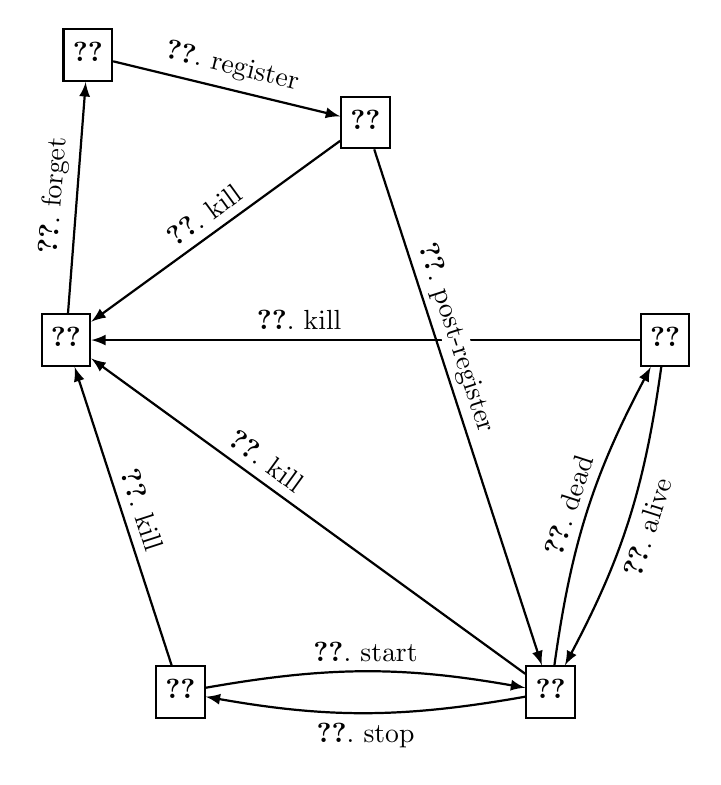
\begin{tikzpicture}
% structure things
% A at 9:30
% B at 12
% ...
% E at 7:30
\foreach \name/\angle/\text in {E/234/E, A/162/A, 
                               B/90/B, C/18/C, D/-54/D}
    \node[circle,draw=white,fill=white,text=white] (\name) at (\angle:4cm) {\text};
\node[circle,draw=white,fill=white,text=white] (F) at (126:6cm) {F};

% Place rectangles for the states
\node[rectangle,minimum height=\baselineskip,draw=black,thick] (unknown)      at (F) {\strut \ref{srvstate:unknown}};
\node[rectangle,minimum height=\baselineskip,draw=black,thick] (assigned)     at (B) {\strut \ref{srvstate:assigned}};
\node[rectangle,minimum height=\baselineskip,draw=black,thick] (notavailable) at (C) {\strut \ref{srvstate:notavailable}};
\node[rectangle,minimum height=\baselineskip,draw=black,thick] (available)    at (D) {\strut \ref{srvstate:available}};
\node[rectangle,minimum height=\baselineskip,draw=black,thick] (shutdown)     at (E) {\strut \ref{srvstate:shutdown}};
\node[rectangle,minimum height=\baselineskip,draw=black,thick] (killed)       at (A) {\strut \ref{srvstate:killed}};

% State transitions
\draw[->,>=latex,thick] (unknown) to node[midway,above,sloped] {\ref{srvtrans:reg}.~register} (assigned);
\draw[->,>=latex,thick] (killed) to node[midway,above,sloped] {\ref{srvtrans:forget}.~forget} (unknown);

\draw[->,>=latex,thick] (notavailable) edge [bend left=10] node[midway,below,sloped] {\ref{srvtrans:alive}.~alive} (available);
\draw[->,>=latex,thick] (available) edge [bend left=10] node[midway,above,sloped] {\ref{srvtrans:dead}.~dead} (notavailable);

\draw[->,>=latex,thick] (available) edge [bend left=10] node[midway,below,sloped] {\ref{srvtrans:stop}.~stop} (shutdown);
\draw[->,>=latex,thick] (shutdown) edge [bend left=10] node[midway,above,sloped] {\ref{srvtrans:start}.~start} (available);

\draw[->,>=latex,thick] (assigned) to node[midway,above,sloped] {\ref{srvtrans:kill}.~kill} (killed);
\draw[->,>=latex,thick] (notavailable) to node[midway,above,sloped,xshift=-24pt] {\ref{srvtrans:kill}.~kill} (killed);
\draw[->,>=latex,thick] (available) to node[midway,above,sloped,xshift=-24pt] {\ref{srvtrans:kill}.~kill} (killed);
\draw[->,>=latex,thick] (shutdown) to node[midway,above,sloped] {\ref{srvtrans:kill}.~kill} (killed);

\draw[->,>=latex,thick] (assigned) -- (available) node[midway,above,sloped,draw=white,fill=white,text=black,rectangle,inner sep=0pt,xshift=-24pt,yshift=2pt] {\ref{srvtrans:postreg}.~post-register};
\end{tikzpicture}
\end{center}
\caption{XXX}
\label{fig:daemon-state-machine}
\end{figure}

\begin{enumerate}[noitemsep]
\item \label{srvtrans:reg} Registration
\item \label{srvtrans:postreg} Post Registration
\item \label{srvtrans:start} Start
\item \label{srvtrans:stop} Stop
\item \label{srvtrans:alive} Alive
\item \label{srvtrans:dead} Dead
\item \label{srvtrans:kill} Kill
\item \label{srvtrans:forget} Forget
\end{enumerate}

\section{Command Reference}
\label{sec:mem:commands}


\part{For Hackers}
\label{part:for-hackers}
\chapter{Writing Client Bindings}
\label{chap:writing-bindigs}


\part{API Reference}
\label{part:api-ref}
\chapter{C API}

\section{Client Library}
% Copyright (c) 2013-2014, Cornell University
% All rights reserved.
%
% Redistribution and use in source and binary forms, with or without
% modification, are permitted provided that the following conditions are met:
%
%     * Redistributions of source code must retain the above copyright notice,
%       this list of conditions and the following disclaimer.
%     * Redistributions in binary form must reproduce the above copyright
%       notice, this list of conditions and the following disclaimer in the
%       documentation and/or other materials provided with the distribution.
%     * Neither the name of HyperDex nor the names of its contributors may be
%       used to endorse or promote products derived from this software without
%       specific prior written permission.
%
% THIS SOFTWARE IS PROVIDED BY THE COPYRIGHT HOLDERS AND CONTRIBUTORS "AS IS"
% AND ANY EXPRESS OR IMPLIED WARRANTIES, INCLUDING, BUT NOT LIMITED TO, THE
% IMPLIED WARRANTIES OF MERCHANTABILITY AND FITNESS FOR A PARTICULAR PURPOSE ARE
% DISCLAIMED. IN NO EVENT SHALL THE COPYRIGHT OWNER OR CONTRIBUTORS BE LIABLE
% FOR ANY DIRECT, INDIRECT, INCIDENTAL, SPECIAL, EXEMPLARY, OR CONSEQUENTIAL
% DAMAGES (INCLUDING, BUT NOT LIMITED TO, PROCUREMENT OF SUBSTITUTE GOODS OR
% SERVICES; LOSS OF USE, DATA, OR PROFITS; OR BUSINESS INTERRUPTION) HOWEVER
% CAUSED AND ON ANY THEORY OF LIABILITY, WHETHER IN CONTRACT, STRICT LIABILITY,
% OR TORT (INCLUDING NEGLIGENCE OR OTHERWISE) ARISING IN ANY WAY OUT OF THE USE
% OF THIS SOFTWARE, EVEN IF ADVISED OF THE POSSIBILITY OF SUCH DAMAGE.

% This LaTeX file is generated by bindings/c.py

%%%%%%%%%%%%%%%%%%%% get %%%%%%%%%%%%%%%%%%%%
\pagebreak
\subsubsection{\code{get}}
\label{api:c:get}
\index{get!C API}
Retreive the object with key "key" from space "space".

\input{api/shards/one-rtt}

\input{api/shards/linearizable}


\paragraph{Definition:}
\begin{ccode}
int64_t hyperdex_client_get(struct hyperdex_client* client,
        const char* space,
        const char* key, size_t key_sz,
        enum hyperdex_client_returncode* status,
        const struct hyperdex_client_attribute** attrs, size_t* attrs_sz);
\end{ccode}

\paragraph{Parameters:}
\begin{itemize}[noitemsep]
\item \code{space}\\
The name of the space as a c-string.
\item \code{key}, \code{key\_sz}\\
The key for the operation where \code{key} is a bytestring and \code{key\_sz} specifies the number of bytes in \code{key}.
\end{itemize}

\paragraph{Returns:}
\begin{itemize}[noitemsep]
\item \code{status}\\
The status of the operation.  The client library will fill in this variable before returning this operation's request id from \code{hyperdex\_client\_loop}.  The pointer must remain valid until then, and the pointer should not be aliased to the status for any other outstanding operation.
\item \code{attrs}, \code{attrs\_sz}\\
An array of attributes that comprise a returned object.  The application must free the returned values with \code{hyperdex\_client\_destroy\_attrs}.  The pointers must remain valid until the operation completes.
\end{itemize}

%%%%%%%%%%%%%%%%%%%% put %%%%%%%%%%%%%%%%%%%%
\pagebreak
\subsubsection{\code{put}}
\label{api:c:put}
\index{put!C API}
Store or update an object by key.  The object's attributes will be set to the
values specified by \code{attrs}.
\input{\topdir/client/fragments/no_fail}


\paragraph{Definition:}
\begin{ccode}
int64_t hyperdex_client_put(struct hyperdex_client* client,
        const char* space,
        const char* key, size_t key_sz,
        const struct hyperdex_client_attribute* attrs, size_t attrs_sz,
        enum hyperdex_client_returncode* status);
\end{ccode}

\paragraph{Parameters:}
\begin{itemize}[noitemsep]
\item \code{space}\\
The name of the space as a c-string.
\item \code{key}, \code{key\_sz}\\
The key for the operation where \code{key} is a bytestring and \code{key\_sz} specifies the number of bytes in \code{key}.
\item \code{attrs}, \code{attrs\_sz}\\
The set of attributes to modify and their respective values.  \code{attrs} points to an array of length \code{attrs\_sz}.
\end{itemize}

\paragraph{Returns:}
\begin{itemize}[noitemsep]
\item \code{status}\\
The status of the operation.  The client library will fill in this variable before returning this operation's request id from \code{hyperdex\_client\_loop}.  The pointer must remain valid until then, and the pointer should not be aliased to the status for any other outstanding operation.
\end{itemize}

%%%%%%%%%%%%%%%%%%%% cond_put %%%%%%%%%%%%%%%%%%%%
\pagebreak
\subsubsection{\code{cond\_put}}
\label{api:c:cond_put}
\index{cond\_put!C API}
Conditionally update an the object stored under \code{key} in \code{space}.
Existing values will be overwritten with the values specified by \code{attrs}.
Values not specified by \code{attrs} will remain unchanged.
\input{\topdir/client/fragments/fail_if_not_found}

\input{\topdir/client/fragments/conditional}


\paragraph{Definition:}
\begin{ccode}
int64_t hyperdex_client_cond_put(struct hyperdex_client* client,
        const char* space,
        const char* key, size_t key_sz,
        const struct hyperdex_client_attribute_check* checks, size_t checks_sz,
        const struct hyperdex_client_attribute* attrs, size_t attrs_sz,
        enum hyperdex_client_returncode* status);
\end{ccode}

\paragraph{Parameters:}
\begin{itemize}[noitemsep]
\item \code{space}\\
The name of the space as a c-string.
\item \code{key}, \code{key\_sz}\\
The key for the operation where \code{key} is a bytestring and \code{key\_sz} specifies the number of bytes in \code{key}.
\item \code{checks}, \code{checks\_sz}\\
A set of predicates to check against.  \code{checks} points to an array of length \code{checks\_sz}.
\item \code{attrs}, \code{attrs\_sz}\\
The set of attributes to modify and their respective values.  \code{attrs} points to an array of length \code{attrs\_sz}.
\end{itemize}

\paragraph{Returns:}
\begin{itemize}[noitemsep]
\item \code{status}\\
The status of the operation.  The client library will fill in this variable before returning this operation's request id from \code{hyperdex\_client\_loop}.  The pointer must remain valid until then, and the pointer should not be aliased to the status for any other outstanding operation.
\end{itemize}

%%%%%%%%%%%%%%%%%%%% put_if_not_exist %%%%%%%%%%%%%%%%%%%%
\pagebreak
\subsubsection{\code{put\_if\_not\_exist}}
\label{api:c:put_if_not_exist}
\index{put\_if\_not\_exist!C API}
Store an object in space "space" under key "key" if and only if it does not
already exist.

The object will be create, and the attributes specified by \texttt{attrs} will
be set to their respective values.  Any attributes not specified by
\texttt{attrs} will be initialized to their default values.  The check is atomic
with the write, and is guaranteed to never overwrite an existing object.

\input{api/shards/chain-rtt}

\input{api/shards/linearizable}


\paragraph{Definition:}
\begin{ccode}
int64_t hyperdex_client_put_if_not_exist(struct hyperdex_client* client,
        const char* space,
        const char* key, size_t key_sz,
        const struct hyperdex_client_attribute* attrs, size_t attrs_sz,
        enum hyperdex_client_returncode* status);
\end{ccode}

\paragraph{Parameters:}
\begin{itemize}[noitemsep]
\item \code{space}\\
The name of the space as a c-string.
\item \code{key}, \code{key\_sz}\\
The key for the operation where \code{key} is a bytestring and \code{key\_sz} specifies the number of bytes in \code{key}.
\item \code{attrs}, \code{attrs\_sz}\\
The set of attributes to modify and their respective values.  \code{attrs} points to an array of length \code{attrs\_sz}.
\end{itemize}

\paragraph{Returns:}
\begin{itemize}[noitemsep]
\item \code{status}\\
The status of the operation.  The client library will fill in this variable before returning this operation's request id from \code{hyperdex\_client\_loop}.  The pointer must remain valid until then, and the pointer should not be aliased to the status for any other outstanding operation.
\end{itemize}

%%%%%%%%%%%%%%%%%%%% del %%%%%%%%%%%%%%%%%%%%
\pagebreak
\subsubsection{\code{del}}
\label{api:c:del}
\index{del!C API}
Delete an object by key.

%%% Generated below here
\paragraph{Behavior:}
\begin{itemize}[noitemsep]
\input{\topdir/api/fragments/erase}
\end{itemize}


\paragraph{Definition:}
\begin{ccode}
int64_t hyperdex_client_del(struct hyperdex_client* client,
        const char* space,
        const char* key, size_t key_sz,
        enum hyperdex_client_returncode* status);
\end{ccode}

\paragraph{Parameters:}
\begin{itemize}[noitemsep]
\item \code{space}\\
The name of the space as a c-string.
\item \code{key}, \code{key\_sz}\\
The key for the operation where \code{key} is a bytestring and \code{key\_sz} specifies the number of bytes in \code{key}.
\end{itemize}

\paragraph{Returns:}
\begin{itemize}[noitemsep]
\item \code{status}\\
The status of the operation.  The client library will fill in this variable before returning this operation's request id from \code{hyperdex\_client\_loop}.  The pointer must remain valid until then, and the pointer should not be aliased to the status for any other outstanding operation.
\end{itemize}

%%%%%%%%%%%%%%%%%%%% cond_del %%%%%%%%%%%%%%%%%%%%
\pagebreak
\subsubsection{\code{cond\_del}}
\label{api:c:cond_del}
\index{cond\_del!C API}
Conditionally delete an object by key.

%%% Generated below here
\paragraph{Behavior:}
\begin{itemize}[noitemsep]
\input{\topdir/api/fragments/erase}
\input{\topdir/api/fragments/conditional}
\end{itemize}


\paragraph{Definition:}
\begin{ccode}
int64_t hyperdex_client_cond_del(struct hyperdex_client* client,
        const char* space,
        const char* key, size_t key_sz,
        const struct hyperdex_client_attribute_check* checks, size_t checks_sz,
        enum hyperdex_client_returncode* status);
\end{ccode}

\paragraph{Parameters:}
\begin{itemize}[noitemsep]
\item \code{space}\\
The name of the space as a c-string.
\item \code{key}, \code{key\_sz}\\
The key for the operation where \code{key} is a bytestring and \code{key\_sz} specifies the number of bytes in \code{key}.
\item \code{checks}, \code{checks\_sz}\\
A set of predicates to check against.  \code{checks} points to an array of length \code{checks\_sz}.
\end{itemize}

\paragraph{Returns:}
\begin{itemize}[noitemsep]
\item \code{status}\\
The status of the operation.  The client library will fill in this variable before returning this operation's request id from \code{hyperdex\_client\_loop}.  The pointer must remain valid until then, and the pointer should not be aliased to the status for any other outstanding operation.
\end{itemize}

%%%%%%%%%%%%%%%%%%%% atomic_add %%%%%%%%%%%%%%%%%%%%
\pagebreak
\subsubsection{\code{atomic\_add}}
\label{api:c:atomic_add}
\index{atomic\_add!C API}
Add the specified number to the existing value for each attribute.
\input{\topdir/client/fragments/fail_if_not_found}


\paragraph{Definition:}
\begin{ccode}
int64_t hyperdex_client_atomic_add(struct hyperdex_client* client,
        const char* space,
        const char* key, size_t key_sz,
        const struct hyperdex_client_attribute* attrs, size_t attrs_sz,
        enum hyperdex_client_returncode* status);
\end{ccode}

\paragraph{Parameters:}
\begin{itemize}[noitemsep]
\item \code{space}\\
The name of the space as a c-string.
\item \code{key}, \code{key\_sz}\\
The key for the operation where \code{key} is a bytestring and \code{key\_sz} specifies the number of bytes in \code{key}.
\item \code{attrs}, \code{attrs\_sz}\\
The set of attributes to modify and their respective values.  \code{attrs} points to an array of length \code{attrs\_sz}.
\end{itemize}

\paragraph{Returns:}
\begin{itemize}[noitemsep]
\item \code{status}\\
The status of the operation.  The client library will fill in this variable before returning this operation's request id from \code{hyperdex\_client\_loop}.  The pointer must remain valid until then, and the pointer should not be aliased to the status for any other outstanding operation.
\end{itemize}

%%%%%%%%%%%%%%%%%%%% cond_atomic_add %%%%%%%%%%%%%%%%%%%%
\pagebreak
\subsubsection{\code{cond\_atomic\_add}}
\label{api:c:cond_atomic_add}
\index{cond\_atomic\_add!C API}
Conditionally add the specified number to the existing value for each attribute.

%%% Generated below here
\paragraph{Behavior:}
\begin{itemize}[noitemsep]
\input{\topdir/api/fragments/fail_if_not_found}
\input{\topdir/api/fragments/conditional}
\end{itemize}


\paragraph{Definition:}
\begin{ccode}
int64_t hyperdex_client_cond_atomic_add(struct hyperdex_client* client,
        const char* space,
        const char* key, size_t key_sz,
        const struct hyperdex_client_attribute_check* checks, size_t checks_sz,
        const struct hyperdex_client_attribute* attrs, size_t attrs_sz,
        enum hyperdex_client_returncode* status);
\end{ccode}

\paragraph{Parameters:}
\begin{itemize}[noitemsep]
\item \code{space}\\
The name of the space as a c-string.
\item \code{key}, \code{key\_sz}\\
The key for the operation where \code{key} is a bytestring and \code{key\_sz} specifies the number of bytes in \code{key}.
\item \code{checks}, \code{checks\_sz}\\
A set of predicates to check against.  \code{checks} points to an array of length \code{checks\_sz}.
\item \code{attrs}, \code{attrs\_sz}\\
The set of attributes to modify and their respective values.  \code{attrs} points to an array of length \code{attrs\_sz}.
\end{itemize}

\paragraph{Returns:}
\begin{itemize}[noitemsep]
\item \code{status}\\
The status of the operation.  The client library will fill in this variable before returning this operation's request id from \code{hyperdex\_client\_loop}.  The pointer must remain valid until then, and the pointer should not be aliased to the status for any other outstanding operation.
\end{itemize}

%%%%%%%%%%%%%%%%%%%% atomic_sub %%%%%%%%%%%%%%%%%%%%
\pagebreak
\subsubsection{\code{atomic\_sub}}
\label{api:c:atomic_sub}
\index{atomic\_sub!C API}
Subtract the specified number from the existing value for each attribute.

%%% Generated below here
\paragraph{Behavior:}
\begin{itemize}[noitemsep]
\input{\topdir/api/fragments/fail_if_not_found}
\end{itemize}


\paragraph{Definition:}
\begin{ccode}
int64_t hyperdex_client_atomic_sub(struct hyperdex_client* client,
        const char* space,
        const char* key, size_t key_sz,
        const struct hyperdex_client_attribute* attrs, size_t attrs_sz,
        enum hyperdex_client_returncode* status);
\end{ccode}

\paragraph{Parameters:}
\begin{itemize}[noitemsep]
\item \code{space}\\
The name of the space as a c-string.
\item \code{key}, \code{key\_sz}\\
The key for the operation where \code{key} is a bytestring and \code{key\_sz} specifies the number of bytes in \code{key}.
\item \code{attrs}, \code{attrs\_sz}\\
The set of attributes to modify and their respective values.  \code{attrs} points to an array of length \code{attrs\_sz}.
\end{itemize}

\paragraph{Returns:}
\begin{itemize}[noitemsep]
\item \code{status}\\
The status of the operation.  The client library will fill in this variable before returning this operation's request id from \code{hyperdex\_client\_loop}.  The pointer must remain valid until then, and the pointer should not be aliased to the status for any other outstanding operation.
\end{itemize}

%%%%%%%%%%%%%%%%%%%% cond_atomic_sub %%%%%%%%%%%%%%%%%%%%
\pagebreak
\subsubsection{\code{cond\_atomic\_sub}}
\label{api:c:cond_atomic_sub}
\index{cond\_atomic\_sub!C API}
Conditionally subtract the specified number from the existing value for each attribute.

%%% Generated below here
\paragraph{Behavior:}
\begin{itemize}[noitemsep]
\input{\topdir/api/fragments/fail_if_not_found}
\input{\topdir/api/fragments/conditional}
\end{itemize}


\paragraph{Definition:}
\begin{ccode}
int64_t hyperdex_client_cond_atomic_sub(struct hyperdex_client* client,
        const char* space,
        const char* key, size_t key_sz,
        const struct hyperdex_client_attribute_check* checks, size_t checks_sz,
        const struct hyperdex_client_attribute* attrs, size_t attrs_sz,
        enum hyperdex_client_returncode* status);
\end{ccode}

\paragraph{Parameters:}
\begin{itemize}[noitemsep]
\item \code{space}\\
The name of the space as a c-string.
\item \code{key}, \code{key\_sz}\\
The key for the operation where \code{key} is a bytestring and \code{key\_sz} specifies the number of bytes in \code{key}.
\item \code{checks}, \code{checks\_sz}\\
A set of predicates to check against.  \code{checks} points to an array of length \code{checks\_sz}.
\item \code{attrs}, \code{attrs\_sz}\\
The set of attributes to modify and their respective values.  \code{attrs} points to an array of length \code{attrs\_sz}.
\end{itemize}

\paragraph{Returns:}
\begin{itemize}[noitemsep]
\item \code{status}\\
The status of the operation.  The client library will fill in this variable before returning this operation's request id from \code{hyperdex\_client\_loop}.  The pointer must remain valid until then, and the pointer should not be aliased to the status for any other outstanding operation.
\end{itemize}

%%%%%%%%%%%%%%%%%%%% atomic_mul %%%%%%%%%%%%%%%%%%%%
\pagebreak
\subsubsection{\code{atomic\_mul}}
\label{api:c:atomic_mul}
\index{atomic\_mul!C API}
\input{\topdir/api/desc/atomic_mul}

\paragraph{Definition:}
\begin{ccode}
int64_t hyperdex_client_atomic_mul(struct hyperdex_client* client,
        const char* space,
        const char* key, size_t key_sz,
        const struct hyperdex_client_attribute* attrs, size_t attrs_sz,
        enum hyperdex_client_returncode* status);
\end{ccode}

\paragraph{Parameters:}
\begin{itemize}[noitemsep]
\item \code{space}\\
The name of the space as a c-string.
\item \code{key}, \code{key\_sz}\\
The key for the operation where \code{key} is a bytestring and \code{key\_sz} specifies the number of bytes in \code{key}.
\item \code{attrs}, \code{attrs\_sz}\\
The set of attributes to modify and their respective values.  \code{attrs} points to an array of length \code{attrs\_sz}.
\end{itemize}

\paragraph{Returns:}
\begin{itemize}[noitemsep]
\item \code{status}\\
The status of the operation.  The client library will fill in this variable before returning this operation's request id from \code{hyperdex\_client\_loop}.  The pointer must remain valid until then, and the pointer should not be aliased to the status for any other outstanding operation.
\end{itemize}

%%%%%%%%%%%%%%%%%%%% cond_atomic_mul %%%%%%%%%%%%%%%%%%%%
\pagebreak
\subsubsection{\code{cond\_atomic\_mul}}
\label{api:c:cond_atomic_mul}
\index{cond\_atomic\_mul!C API}
Multiply the existing value by the specified number for each attribute if and
only if the \code{checks} hold on the object.
\input{\topdir/client/fragments/fail_if_not_found}

\input{\topdir/client/fragments/conditional}


\paragraph{Definition:}
\begin{ccode}
int64_t hyperdex_client_cond_atomic_mul(struct hyperdex_client* client,
        const char* space,
        const char* key, size_t key_sz,
        const struct hyperdex_client_attribute_check* checks, size_t checks_sz,
        const struct hyperdex_client_attribute* attrs, size_t attrs_sz,
        enum hyperdex_client_returncode* status);
\end{ccode}

\paragraph{Parameters:}
\begin{itemize}[noitemsep]
\item \code{space}\\
The name of the space as a c-string.
\item \code{key}, \code{key\_sz}\\
The key for the operation where \code{key} is a bytestring and \code{key\_sz} specifies the number of bytes in \code{key}.
\item \code{checks}, \code{checks\_sz}\\
A set of predicates to check against.  \code{checks} points to an array of length \code{checks\_sz}.
\item \code{attrs}, \code{attrs\_sz}\\
The set of attributes to modify and their respective values.  \code{attrs} points to an array of length \code{attrs\_sz}.
\end{itemize}

\paragraph{Returns:}
\begin{itemize}[noitemsep]
\item \code{status}\\
The status of the operation.  The client library will fill in this variable before returning this operation's request id from \code{hyperdex\_client\_loop}.  The pointer must remain valid until then, and the pointer should not be aliased to the status for any other outstanding operation.
\end{itemize}

%%%%%%%%%%%%%%%%%%%% atomic_div %%%%%%%%%%%%%%%%%%%%
\pagebreak
\subsubsection{\code{atomic\_div}}
\label{api:c:atomic_div}
\index{atomic\_div!C API}
Divide the existing value by the number specified for each attribute.

The division is atomic with the write.  If the object does not exist, the
operation will fail.

\input{\topdir/api/shards/chain-rtt}

\input{\topdir/api/shards/linearizable}


\paragraph{Definition:}
\begin{ccode}
int64_t hyperdex_client_atomic_div(struct hyperdex_client* client,
        const char* space,
        const char* key, size_t key_sz,
        const struct hyperdex_client_attribute* attrs, size_t attrs_sz,
        enum hyperdex_client_returncode* status);
\end{ccode}

\paragraph{Parameters:}
\begin{itemize}[noitemsep]
\item \code{space}\\
The name of the space as a c-string.
\item \code{key}, \code{key\_sz}\\
The key for the operation where \code{key} is a bytestring and \code{key\_sz} specifies the number of bytes in \code{key}.
\item \code{attrs}, \code{attrs\_sz}\\
The set of attributes to modify and their respective values.  \code{attrs} points to an array of length \code{attrs\_sz}.
\end{itemize}

\paragraph{Returns:}
\begin{itemize}[noitemsep]
\item \code{status}\\
The status of the operation.  The client library will fill in this variable before returning this operation's request id from \code{hyperdex\_client\_loop}.  The pointer must remain valid until then, and the pointer should not be aliased to the status for any other outstanding operation.
\end{itemize}

%%%%%%%%%%%%%%%%%%%% cond_atomic_div %%%%%%%%%%%%%%%%%%%%
\pagebreak
\subsubsection{\code{cond\_atomic\_div}}
\label{api:c:cond_atomic_div}
\index{cond\_atomic\_div!C API}
\input{\topdir/api/desc/cond_atomic_div}

\paragraph{Definition:}
\begin{ccode}
int64_t hyperdex_client_cond_atomic_div(struct hyperdex_client* client,
        const char* space,
        const char* key, size_t key_sz,
        const struct hyperdex_client_attribute_check* checks, size_t checks_sz,
        const struct hyperdex_client_attribute* attrs, size_t attrs_sz,
        enum hyperdex_client_returncode* status);
\end{ccode}

\paragraph{Parameters:}
\begin{itemize}[noitemsep]
\item \code{space}\\
The name of the space as a c-string.
\item \code{key}, \code{key\_sz}\\
The key for the operation where \code{key} is a bytestring and \code{key\_sz} specifies the number of bytes in \code{key}.
\item \code{checks}, \code{checks\_sz}\\
A set of predicates to check against.  \code{checks} points to an array of length \code{checks\_sz}.
\item \code{attrs}, \code{attrs\_sz}\\
The set of attributes to modify and their respective values.  \code{attrs} points to an array of length \code{attrs\_sz}.
\end{itemize}

\paragraph{Returns:}
\begin{itemize}[noitemsep]
\item \code{status}\\
The status of the operation.  The client library will fill in this variable before returning this operation's request id from \code{hyperdex\_client\_loop}.  The pointer must remain valid until then, and the pointer should not be aliased to the status for any other outstanding operation.
\end{itemize}

%%%%%%%%%%%%%%%%%%%% atomic_mod %%%%%%%%%%%%%%%%%%%%
\pagebreak
\subsubsection{\code{atomic\_mod}}
\label{api:c:atomic_mod}
\index{atomic\_mod!C API}
Store the existing value modulo the specified number for each attribute.
\input{\topdir/client/fragments/fail_if_not_found}


\paragraph{Definition:}
\begin{ccode}
int64_t hyperdex_client_atomic_mod(struct hyperdex_client* client,
        const char* space,
        const char* key, size_t key_sz,
        const struct hyperdex_client_attribute* attrs, size_t attrs_sz,
        enum hyperdex_client_returncode* status);
\end{ccode}

\paragraph{Parameters:}
\begin{itemize}[noitemsep]
\item \code{space}\\
The name of the space as a c-string.
\item \code{key}, \code{key\_sz}\\
The key for the operation where \code{key} is a bytestring and \code{key\_sz} specifies the number of bytes in \code{key}.
\item \code{attrs}, \code{attrs\_sz}\\
The set of attributes to modify and their respective values.  \code{attrs} points to an array of length \code{attrs\_sz}.
\end{itemize}

\paragraph{Returns:}
\begin{itemize}[noitemsep]
\item \code{status}\\
The status of the operation.  The client library will fill in this variable before returning this operation's request id from \code{hyperdex\_client\_loop}.  The pointer must remain valid until then, and the pointer should not be aliased to the status for any other outstanding operation.
\end{itemize}

%%%%%%%%%%%%%%%%%%%% cond_atomic_mod %%%%%%%%%%%%%%%%%%%%
\pagebreak
\subsubsection{\code{cond\_atomic\_mod}}
\label{api:c:cond_atomic_mod}
\index{cond\_atomic\_mod!C API}
Conditionally store the existing value modulo the specified number for each
attribute.

%%% Generated below here
\paragraph{Behavior:}
\begin{itemize}[noitemsep]
\input{\topdir/api/fragments/fail_if_not_found}
\input{\topdir/api/fragments/conditional}
\end{itemize}


\paragraph{Definition:}
\begin{ccode}
int64_t hyperdex_client_cond_atomic_mod(struct hyperdex_client* client,
        const char* space,
        const char* key, size_t key_sz,
        const struct hyperdex_client_attribute_check* checks, size_t checks_sz,
        const struct hyperdex_client_attribute* attrs, size_t attrs_sz,
        enum hyperdex_client_returncode* status);
\end{ccode}

\paragraph{Parameters:}
\begin{itemize}[noitemsep]
\item \code{space}\\
The name of the space as a c-string.
\item \code{key}, \code{key\_sz}\\
The key for the operation where \code{key} is a bytestring and \code{key\_sz} specifies the number of bytes in \code{key}.
\item \code{checks}, \code{checks\_sz}\\
A set of predicates to check against.  \code{checks} points to an array of length \code{checks\_sz}.
\item \code{attrs}, \code{attrs\_sz}\\
The set of attributes to modify and their respective values.  \code{attrs} points to an array of length \code{attrs\_sz}.
\end{itemize}

\paragraph{Returns:}
\begin{itemize}[noitemsep]
\item \code{status}\\
The status of the operation.  The client library will fill in this variable before returning this operation's request id from \code{hyperdex\_client\_loop}.  The pointer must remain valid until then, and the pointer should not be aliased to the status for any other outstanding operation.
\end{itemize}

%%%%%%%%%%%%%%%%%%%% atomic_and %%%%%%%%%%%%%%%%%%%%
\pagebreak
\subsubsection{\code{atomic\_and}}
\label{api:c:atomic_and}
\index{atomic\_and!C API}
Store the bitwise AND of the existing value and the specified number for
each attribute.
\input{\topdir/client/fragments/fail_if_not_found}


\paragraph{Definition:}
\begin{ccode}
int64_t hyperdex_client_atomic_and(struct hyperdex_client* client,
        const char* space,
        const char* key, size_t key_sz,
        const struct hyperdex_client_attribute* attrs, size_t attrs_sz,
        enum hyperdex_client_returncode* status);
\end{ccode}

\paragraph{Parameters:}
\begin{itemize}[noitemsep]
\item \code{space}\\
The name of the space as a c-string.
\item \code{key}, \code{key\_sz}\\
The key for the operation where \code{key} is a bytestring and \code{key\_sz} specifies the number of bytes in \code{key}.
\item \code{attrs}, \code{attrs\_sz}\\
The set of attributes to modify and their respective values.  \code{attrs} points to an array of length \code{attrs\_sz}.
\end{itemize}

\paragraph{Returns:}
\begin{itemize}[noitemsep]
\item \code{status}\\
The status of the operation.  The client library will fill in this variable before returning this operation's request id from \code{hyperdex\_client\_loop}.  The pointer must remain valid until then, and the pointer should not be aliased to the status for any other outstanding operation.
\end{itemize}

%%%%%%%%%%%%%%%%%%%% cond_atomic_and %%%%%%%%%%%%%%%%%%%%
\pagebreak
\subsubsection{\code{cond\_atomic\_and}}
\label{api:c:cond_atomic_and}
\index{cond\_atomic\_and!C API}
Conditionally store the bitwise AND of the existing value and the specified
number for each attribute.

%%% Generated below here
\paragraph{Behavior:}
\begin{itemize}[noitemsep]
\input{api/fragments/fail_if_not_found}
\input{api/fragments/conditional}
\end{itemize}


\paragraph{Definition:}
\begin{ccode}
int64_t hyperdex_client_cond_atomic_and(struct hyperdex_client* client,
        const char* space,
        const char* key, size_t key_sz,
        const struct hyperdex_client_attribute_check* checks, size_t checks_sz,
        const struct hyperdex_client_attribute* attrs, size_t attrs_sz,
        enum hyperdex_client_returncode* status);
\end{ccode}

\paragraph{Parameters:}
\begin{itemize}[noitemsep]
\item \code{space}\\
The name of the space as a c-string.
\item \code{key}, \code{key\_sz}\\
The key for the operation where \code{key} is a bytestring and \code{key\_sz} specifies the number of bytes in \code{key}.
\item \code{checks}, \code{checks\_sz}\\
A set of predicates to check against.  \code{checks} points to an array of length \code{checks\_sz}.
\item \code{attrs}, \code{attrs\_sz}\\
The set of attributes to modify and their respective values.  \code{attrs} points to an array of length \code{attrs\_sz}.
\end{itemize}

\paragraph{Returns:}
\begin{itemize}[noitemsep]
\item \code{status}\\
The status of the operation.  The client library will fill in this variable before returning this operation's request id from \code{hyperdex\_client\_loop}.  The pointer must remain valid until then, and the pointer should not be aliased to the status for any other outstanding operation.
\end{itemize}

%%%%%%%%%%%%%%%%%%%% atomic_or %%%%%%%%%%%%%%%%%%%%
\pagebreak
\subsubsection{\code{atomic\_or}}
\label{api:c:atomic_or}
\index{atomic\_or!C API}
Store the bitwise OR of the existing value and the specified number for each
attribute.

%%% Generated below here
\paragraph{Behavior:}
\begin{itemize}[noitemsep]
\input{\topdir/api/fragments/fail_if_not_found}
\end{itemize}


\paragraph{Definition:}
\begin{ccode}
int64_t hyperdex_client_atomic_or(struct hyperdex_client* client,
        const char* space,
        const char* key, size_t key_sz,
        const struct hyperdex_client_attribute* attrs, size_t attrs_sz,
        enum hyperdex_client_returncode* status);
\end{ccode}

\paragraph{Parameters:}
\begin{itemize}[noitemsep]
\item \code{space}\\
The name of the space as a c-string.
\item \code{key}, \code{key\_sz}\\
The key for the operation where \code{key} is a bytestring and \code{key\_sz} specifies the number of bytes in \code{key}.
\item \code{attrs}, \code{attrs\_sz}\\
The set of attributes to modify and their respective values.  \code{attrs} points to an array of length \code{attrs\_sz}.
\end{itemize}

\paragraph{Returns:}
\begin{itemize}[noitemsep]
\item \code{status}\\
The status of the operation.  The client library will fill in this variable before returning this operation's request id from \code{hyperdex\_client\_loop}.  The pointer must remain valid until then, and the pointer should not be aliased to the status for any other outstanding operation.
\end{itemize}

%%%%%%%%%%%%%%%%%%%% cond_atomic_or %%%%%%%%%%%%%%%%%%%%
\pagebreak
\subsubsection{\code{cond\_atomic\_or}}
\label{api:c:cond_atomic_or}
\index{cond\_atomic\_or!C API}
\input{\topdir/api/desc/cond_atomic_or}

\paragraph{Definition:}
\begin{ccode}
int64_t hyperdex_client_cond_atomic_or(struct hyperdex_client* client,
        const char* space,
        const char* key, size_t key_sz,
        const struct hyperdex_client_attribute_check* checks, size_t checks_sz,
        const struct hyperdex_client_attribute* attrs, size_t attrs_sz,
        enum hyperdex_client_returncode* status);
\end{ccode}

\paragraph{Parameters:}
\begin{itemize}[noitemsep]
\item \code{space}\\
The name of the space as a c-string.
\item \code{key}, \code{key\_sz}\\
The key for the operation where \code{key} is a bytestring and \code{key\_sz} specifies the number of bytes in \code{key}.
\item \code{checks}, \code{checks\_sz}\\
A set of predicates to check against.  \code{checks} points to an array of length \code{checks\_sz}.
\item \code{attrs}, \code{attrs\_sz}\\
The set of attributes to modify and their respective values.  \code{attrs} points to an array of length \code{attrs\_sz}.
\end{itemize}

\paragraph{Returns:}
\begin{itemize}[noitemsep]
\item \code{status}\\
The status of the operation.  The client library will fill in this variable before returning this operation's request id from \code{hyperdex\_client\_loop}.  The pointer must remain valid until then, and the pointer should not be aliased to the status for any other outstanding operation.
\end{itemize}

%%%%%%%%%%%%%%%%%%%% atomic_xor %%%%%%%%%%%%%%%%%%%%
\pagebreak
\subsubsection{\code{atomic\_xor}}
\label{api:c:atomic_xor}
\index{atomic\_xor!C API}
Store the bitwise XOR of the existing value and the specified number for each
attribute.
\input{\topdir/client/fragments/fail_if_not_found}


\paragraph{Definition:}
\begin{ccode}
int64_t hyperdex_client_atomic_xor(struct hyperdex_client* client,
        const char* space,
        const char* key, size_t key_sz,
        const struct hyperdex_client_attribute* attrs, size_t attrs_sz,
        enum hyperdex_client_returncode* status);
\end{ccode}

\paragraph{Parameters:}
\begin{itemize}[noitemsep]
\item \code{space}\\
The name of the space as a c-string.
\item \code{key}, \code{key\_sz}\\
The key for the operation where \code{key} is a bytestring and \code{key\_sz} specifies the number of bytes in \code{key}.
\item \code{attrs}, \code{attrs\_sz}\\
The set of attributes to modify and their respective values.  \code{attrs} points to an array of length \code{attrs\_sz}.
\end{itemize}

\paragraph{Returns:}
\begin{itemize}[noitemsep]
\item \code{status}\\
The status of the operation.  The client library will fill in this variable before returning this operation's request id from \code{hyperdex\_client\_loop}.  The pointer must remain valid until then, and the pointer should not be aliased to the status for any other outstanding operation.
\end{itemize}

%%%%%%%%%%%%%%%%%%%% cond_atomic_xor %%%%%%%%%%%%%%%%%%%%
\pagebreak
\subsubsection{\code{cond\_atomic\_xor}}
\label{api:c:cond_atomic_xor}
\index{cond\_atomic\_xor!C API}
Conditionally store the bitwise XOR of the existing value and the specified
number for each attribute.

%%% Generated below here
\paragraph{Behavior:}
\begin{itemize}[noitemsep]
\input{\topdir/api/fragments/fail_if_not_found}
\input{\topdir/api/fragments/conditional}
\end{itemize}


\paragraph{Definition:}
\begin{ccode}
int64_t hyperdex_client_cond_atomic_xor(struct hyperdex_client* client,
        const char* space,
        const char* key, size_t key_sz,
        const struct hyperdex_client_attribute_check* checks, size_t checks_sz,
        const struct hyperdex_client_attribute* attrs, size_t attrs_sz,
        enum hyperdex_client_returncode* status);
\end{ccode}

\paragraph{Parameters:}
\begin{itemize}[noitemsep]
\item \code{space}\\
The name of the space as a c-string.
\item \code{key}, \code{key\_sz}\\
The key for the operation where \code{key} is a bytestring and \code{key\_sz} specifies the number of bytes in \code{key}.
\item \code{checks}, \code{checks\_sz}\\
A set of predicates to check against.  \code{checks} points to an array of length \code{checks\_sz}.
\item \code{attrs}, \code{attrs\_sz}\\
The set of attributes to modify and their respective values.  \code{attrs} points to an array of length \code{attrs\_sz}.
\end{itemize}

\paragraph{Returns:}
\begin{itemize}[noitemsep]
\item \code{status}\\
The status of the operation.  The client library will fill in this variable before returning this operation's request id from \code{hyperdex\_client\_loop}.  The pointer must remain valid until then, and the pointer should not be aliased to the status for any other outstanding operation.
\end{itemize}

%%%%%%%%%%%%%%%%%%%% string_prepend %%%%%%%%%%%%%%%%%%%%
\pagebreak
\subsubsection{\code{string\_prepend}}
\label{api:c:string_prepend}
\index{string\_prepend!C API}
Prepend the specified string to the existing value for each attribute.

%%% Generated below here
\paragraph{Behavior:}
\begin{itemize}[noitemsep]
\input{api/fragments/fail_if_not_found}
\end{itemize}


\paragraph{Definition:}
\begin{ccode}
int64_t hyperdex_client_string_prepend(struct hyperdex_client* client,
        const char* space,
        const char* key, size_t key_sz,
        const struct hyperdex_client_attribute* attrs, size_t attrs_sz,
        enum hyperdex_client_returncode* status);
\end{ccode}

\paragraph{Parameters:}
\begin{itemize}[noitemsep]
\item \code{space}\\
The name of the space as a c-string.
\item \code{key}, \code{key\_sz}\\
The key for the operation where \code{key} is a bytestring and \code{key\_sz} specifies the number of bytes in \code{key}.
\item \code{attrs}, \code{attrs\_sz}\\
The set of attributes to modify and their respective values.  \code{attrs} points to an array of length \code{attrs\_sz}.
\end{itemize}

\paragraph{Returns:}
\begin{itemize}[noitemsep]
\item \code{status}\\
The status of the operation.  The client library will fill in this variable before returning this operation's request id from \code{hyperdex\_client\_loop}.  The pointer must remain valid until then, and the pointer should not be aliased to the status for any other outstanding operation.
\end{itemize}

%%%%%%%%%%%%%%%%%%%% cond_string_prepend %%%%%%%%%%%%%%%%%%%%
\pagebreak
\subsubsection{\code{cond\_string\_prepend}}
\label{api:c:cond_string_prepend}
\index{cond\_string\_prepend!C API}
Conditionally prepend the specified string to the existing value for each
attribute.

%%% Generated below here
\paragraph{Behavior:}
\begin{itemize}[noitemsep]
\input{\topdir/api/fragments/fail_if_not_found}
\input{\topdir/api/fragments/conditional}
\end{itemize}


\paragraph{Definition:}
\begin{ccode}
int64_t hyperdex_client_cond_string_prepend(struct hyperdex_client* client,
        const char* space,
        const char* key, size_t key_sz,
        const struct hyperdex_client_attribute_check* checks, size_t checks_sz,
        const struct hyperdex_client_attribute* attrs, size_t attrs_sz,
        enum hyperdex_client_returncode* status);
\end{ccode}

\paragraph{Parameters:}
\begin{itemize}[noitemsep]
\item \code{space}\\
The name of the space as a c-string.
\item \code{key}, \code{key\_sz}\\
The key for the operation where \code{key} is a bytestring and \code{key\_sz} specifies the number of bytes in \code{key}.
\item \code{checks}, \code{checks\_sz}\\
A set of predicates to check against.  \code{checks} points to an array of length \code{checks\_sz}.
\item \code{attrs}, \code{attrs\_sz}\\
The set of attributes to modify and their respective values.  \code{attrs} points to an array of length \code{attrs\_sz}.
\end{itemize}

\paragraph{Returns:}
\begin{itemize}[noitemsep]
\item \code{status}\\
The status of the operation.  The client library will fill in this variable before returning this operation's request id from \code{hyperdex\_client\_loop}.  The pointer must remain valid until then, and the pointer should not be aliased to the status for any other outstanding operation.
\end{itemize}

%%%%%%%%%%%%%%%%%%%% string_append %%%%%%%%%%%%%%%%%%%%
\pagebreak
\subsubsection{\code{string\_append}}
\label{api:c:string_append}
\index{string\_append!C API}
Append the specified string to the existing value for each attribute.
\input{\topdir/client/fragments/fail_if_not_found}


\paragraph{Definition:}
\begin{ccode}
int64_t hyperdex_client_string_append(struct hyperdex_client* client,
        const char* space,
        const char* key, size_t key_sz,
        const struct hyperdex_client_attribute* attrs, size_t attrs_sz,
        enum hyperdex_client_returncode* status);
\end{ccode}

\paragraph{Parameters:}
\begin{itemize}[noitemsep]
\item \code{space}\\
The name of the space as a c-string.
\item \code{key}, \code{key\_sz}\\
The key for the operation where \code{key} is a bytestring and \code{key\_sz} specifies the number of bytes in \code{key}.
\item \code{attrs}, \code{attrs\_sz}\\
The set of attributes to modify and their respective values.  \code{attrs} points to an array of length \code{attrs\_sz}.
\end{itemize}

\paragraph{Returns:}
\begin{itemize}[noitemsep]
\item \code{status}\\
The status of the operation.  The client library will fill in this variable before returning this operation's request id from \code{hyperdex\_client\_loop}.  The pointer must remain valid until then, and the pointer should not be aliased to the status for any other outstanding operation.
\end{itemize}

%%%%%%%%%%%%%%%%%%%% cond_string_append %%%%%%%%%%%%%%%%%%%%
\pagebreak
\subsubsection{\code{cond\_string\_append}}
\label{api:c:cond_string_append}
\index{cond\_string\_append!C API}
Append the specified string to the existing value for each attribute if and only
if \code{checks} hold on the object.
\input{\topdir/client/fragments/fail_if_not_found}

\input{\topdir/client/fragments/conditional}


\paragraph{Definition:}
\begin{ccode}
int64_t hyperdex_client_cond_string_append(struct hyperdex_client* client,
        const char* space,
        const char* key, size_t key_sz,
        const struct hyperdex_client_attribute_check* checks, size_t checks_sz,
        const struct hyperdex_client_attribute* attrs, size_t attrs_sz,
        enum hyperdex_client_returncode* status);
\end{ccode}

\paragraph{Parameters:}
\begin{itemize}[noitemsep]
\item \code{space}\\
The name of the space as a c-string.
\item \code{key}, \code{key\_sz}\\
The key for the operation where \code{key} is a bytestring and \code{key\_sz} specifies the number of bytes in \code{key}.
\item \code{checks}, \code{checks\_sz}\\
A set of predicates to check against.  \code{checks} points to an array of length \code{checks\_sz}.
\item \code{attrs}, \code{attrs\_sz}\\
The set of attributes to modify and their respective values.  \code{attrs} points to an array of length \code{attrs\_sz}.
\end{itemize}

\paragraph{Returns:}
\begin{itemize}[noitemsep]
\item \code{status}\\
The status of the operation.  The client library will fill in this variable before returning this operation's request id from \code{hyperdex\_client\_loop}.  The pointer must remain valid until then, and the pointer should not be aliased to the status for any other outstanding operation.
\end{itemize}

%%%%%%%%%%%%%%%%%%%% list_lpush %%%%%%%%%%%%%%%%%%%%
\pagebreak
\subsubsection{\code{list\_lpush}}
\label{api:c:list_lpush}
\index{list\_lpush!C API}
Push the specified value onto the front of the list for each attribute.

%%% Generated below here
\paragraph{Behavior:}
\begin{itemize}[noitemsep]
\input{\topdir/api/fragments/fail_if_not_found}
\end{itemize}


\paragraph{Definition:}
\begin{ccode}
int64_t hyperdex_client_list_lpush(struct hyperdex_client* client,
        const char* space,
        const char* key, size_t key_sz,
        const struct hyperdex_client_attribute* attrs, size_t attrs_sz,
        enum hyperdex_client_returncode* status);
\end{ccode}

\paragraph{Parameters:}
\begin{itemize}[noitemsep]
\item \code{space}\\
The name of the space as a c-string.
\item \code{key}, \code{key\_sz}\\
The key for the operation where \code{key} is a bytestring and \code{key\_sz} specifies the number of bytes in \code{key}.
\item \code{attrs}, \code{attrs\_sz}\\
The set of attributes to modify and their respective values.  \code{attrs} points to an array of length \code{attrs\_sz}.
\end{itemize}

\paragraph{Returns:}
\begin{itemize}[noitemsep]
\item \code{status}\\
The status of the operation.  The client library will fill in this variable before returning this operation's request id from \code{hyperdex\_client\_loop}.  The pointer must remain valid until then, and the pointer should not be aliased to the status for any other outstanding operation.
\end{itemize}

%%%%%%%%%%%%%%%%%%%% cond_list_lpush %%%%%%%%%%%%%%%%%%%%
\pagebreak
\subsubsection{\code{cond\_list\_lpush}}
\label{api:c:cond_list_lpush}
\index{cond\_list\_lpush!C API}
Condtitionally push the specified value onto the front of the list for each
attribute.

%%% Generated below here
\paragraph{Behavior:}
\begin{itemize}[noitemsep]
\input{\topdir/api/fragments/fail_if_not_found}
\input{\topdir/api/fragments/conditional}
\end{itemize}


\paragraph{Definition:}
\begin{ccode}
int64_t hyperdex_client_cond_list_lpush(struct hyperdex_client* client,
        const char* space,
        const char* key, size_t key_sz,
        const struct hyperdex_client_attribute_check* checks, size_t checks_sz,
        const struct hyperdex_client_attribute* attrs, size_t attrs_sz,
        enum hyperdex_client_returncode* status);
\end{ccode}

\paragraph{Parameters:}
\begin{itemize}[noitemsep]
\item \code{space}\\
The name of the space as a c-string.
\item \code{key}, \code{key\_sz}\\
The key for the operation where \code{key} is a bytestring and \code{key\_sz} specifies the number of bytes in \code{key}.
\item \code{checks}, \code{checks\_sz}\\
A set of predicates to check against.  \code{checks} points to an array of length \code{checks\_sz}.
\item \code{attrs}, \code{attrs\_sz}\\
The set of attributes to modify and their respective values.  \code{attrs} points to an array of length \code{attrs\_sz}.
\end{itemize}

\paragraph{Returns:}
\begin{itemize}[noitemsep]
\item \code{status}\\
The status of the operation.  The client library will fill in this variable before returning this operation's request id from \code{hyperdex\_client\_loop}.  The pointer must remain valid until then, and the pointer should not be aliased to the status for any other outstanding operation.
\end{itemize}

%%%%%%%%%%%%%%%%%%%% list_rpush %%%%%%%%%%%%%%%%%%%%
\pagebreak
\subsubsection{\code{list\_rpush}}
\label{api:c:list_rpush}
\index{list\_rpush!C API}
Push the specified value onto the back of the list for each attribute.

%%% Generated below here
\paragraph{Behavior:}
\begin{itemize}[noitemsep]
\input{api/fragments/fail_if_not_found}
\end{itemize}


\paragraph{Definition:}
\begin{ccode}
int64_t hyperdex_client_list_rpush(struct hyperdex_client* client,
        const char* space,
        const char* key, size_t key_sz,
        const struct hyperdex_client_attribute* attrs, size_t attrs_sz,
        enum hyperdex_client_returncode* status);
\end{ccode}

\paragraph{Parameters:}
\begin{itemize}[noitemsep]
\item \code{space}\\
The name of the space as a c-string.
\item \code{key}, \code{key\_sz}\\
The key for the operation where \code{key} is a bytestring and \code{key\_sz} specifies the number of bytes in \code{key}.
\item \code{attrs}, \code{attrs\_sz}\\
The set of attributes to modify and their respective values.  \code{attrs} points to an array of length \code{attrs\_sz}.
\end{itemize}

\paragraph{Returns:}
\begin{itemize}[noitemsep]
\item \code{status}\\
The status of the operation.  The client library will fill in this variable before returning this operation's request id from \code{hyperdex\_client\_loop}.  The pointer must remain valid until then, and the pointer should not be aliased to the status for any other outstanding operation.
\end{itemize}

%%%%%%%%%%%%%%%%%%%% cond_list_rpush %%%%%%%%%%%%%%%%%%%%
\pagebreak
\subsubsection{\code{cond\_list\_rpush}}
\label{api:c:cond_list_rpush}
\index{cond\_list\_rpush!C API}
Push the specified value onto the back of the list for each attribute if and
only if the \code{checks} hold on the object.
\input{\topdir/client/fragments/fail_if_not_found}

\input{\topdir/client/fragments/conditional}


\paragraph{Definition:}
\begin{ccode}
int64_t hyperdex_client_cond_list_rpush(struct hyperdex_client* client,
        const char* space,
        const char* key, size_t key_sz,
        const struct hyperdex_client_attribute_check* checks, size_t checks_sz,
        const struct hyperdex_client_attribute* attrs, size_t attrs_sz,
        enum hyperdex_client_returncode* status);
\end{ccode}

\paragraph{Parameters:}
\begin{itemize}[noitemsep]
\item \code{space}\\
The name of the space as a c-string.
\item \code{key}, \code{key\_sz}\\
The key for the operation where \code{key} is a bytestring and \code{key\_sz} specifies the number of bytes in \code{key}.
\item \code{checks}, \code{checks\_sz}\\
A set of predicates to check against.  \code{checks} points to an array of length \code{checks\_sz}.
\item \code{attrs}, \code{attrs\_sz}\\
The set of attributes to modify and their respective values.  \code{attrs} points to an array of length \code{attrs\_sz}.
\end{itemize}

\paragraph{Returns:}
\begin{itemize}[noitemsep]
\item \code{status}\\
The status of the operation.  The client library will fill in this variable before returning this operation's request id from \code{hyperdex\_client\_loop}.  The pointer must remain valid until then, and the pointer should not be aliased to the status for any other outstanding operation.
\end{itemize}

%%%%%%%%%%%%%%%%%%%% set_add %%%%%%%%%%%%%%%%%%%%
\pagebreak
\subsubsection{\code{set\_add}}
\label{api:c:set_add}
\index{set\_add!C API}
Add the specified value to the set for each attribute.

%%% Generated below here
\paragraph{Behavior:}
\begin{itemize}[noitemsep]
\input{\topdir/api/fragments/fail_if_not_found}
\end{itemize}


\paragraph{Definition:}
\begin{ccode}
int64_t hyperdex_client_set_add(struct hyperdex_client* client,
        const char* space,
        const char* key, size_t key_sz,
        const struct hyperdex_client_attribute* attrs, size_t attrs_sz,
        enum hyperdex_client_returncode* status);
\end{ccode}

\paragraph{Parameters:}
\begin{itemize}[noitemsep]
\item \code{space}\\
The name of the space as a c-string.
\item \code{key}, \code{key\_sz}\\
The key for the operation where \code{key} is a bytestring and \code{key\_sz} specifies the number of bytes in \code{key}.
\item \code{attrs}, \code{attrs\_sz}\\
The set of attributes to modify and their respective values.  \code{attrs} points to an array of length \code{attrs\_sz}.
\end{itemize}

\paragraph{Returns:}
\begin{itemize}[noitemsep]
\item \code{status}\\
The status of the operation.  The client library will fill in this variable before returning this operation's request id from \code{hyperdex\_client\_loop}.  The pointer must remain valid until then, and the pointer should not be aliased to the status for any other outstanding operation.
\end{itemize}

%%%%%%%%%%%%%%%%%%%% cond_set_add %%%%%%%%%%%%%%%%%%%%
\pagebreak
\subsubsection{\code{cond\_set\_add}}
\label{api:c:cond_set_add}
\index{cond\_set\_add!C API}
Conditionally add the specified value to the set for each attribute.

%%% Generated below here
\paragraph{Behavior:}
\begin{itemize}[noitemsep]
\input{api/fragments/fail_if_not_found}
\input{api/fragments/conditional}
\end{itemize}


\paragraph{Definition:}
\begin{ccode}
int64_t hyperdex_client_cond_set_add(struct hyperdex_client* client,
        const char* space,
        const char* key, size_t key_sz,
        const struct hyperdex_client_attribute_check* checks, size_t checks_sz,
        const struct hyperdex_client_attribute* attrs, size_t attrs_sz,
        enum hyperdex_client_returncode* status);
\end{ccode}

\paragraph{Parameters:}
\begin{itemize}[noitemsep]
\item \code{space}\\
The name of the space as a c-string.
\item \code{key}, \code{key\_sz}\\
The key for the operation where \code{key} is a bytestring and \code{key\_sz} specifies the number of bytes in \code{key}.
\item \code{checks}, \code{checks\_sz}\\
A set of predicates to check against.  \code{checks} points to an array of length \code{checks\_sz}.
\item \code{attrs}, \code{attrs\_sz}\\
The set of attributes to modify and their respective values.  \code{attrs} points to an array of length \code{attrs\_sz}.
\end{itemize}

\paragraph{Returns:}
\begin{itemize}[noitemsep]
\item \code{status}\\
The status of the operation.  The client library will fill in this variable before returning this operation's request id from \code{hyperdex\_client\_loop}.  The pointer must remain valid until then, and the pointer should not be aliased to the status for any other outstanding operation.
\end{itemize}

%%%%%%%%%%%%%%%%%%%% set_remove %%%%%%%%%%%%%%%%%%%%
\pagebreak
\subsubsection{\code{set\_remove}}
\label{api:c:set_remove}
\index{set\_remove!C API}
Remove the specified value from the set.  If the value is not contained within
the set, this operation will do nothing.

%%% Generated below here
\paragraph{Behavior:}
\begin{itemize}[noitemsep]
\input{api/fragments/fail_if_not_found}
\end{itemize}


\paragraph{Definition:}
\begin{ccode}
int64_t hyperdex_client_set_remove(struct hyperdex_client* client,
        const char* space,
        const char* key, size_t key_sz,
        const struct hyperdex_client_attribute* attrs, size_t attrs_sz,
        enum hyperdex_client_returncode* status);
\end{ccode}

\paragraph{Parameters:}
\begin{itemize}[noitemsep]
\item \code{space}\\
The name of the space as a c-string.
\item \code{key}, \code{key\_sz}\\
The key for the operation where \code{key} is a bytestring and \code{key\_sz} specifies the number of bytes in \code{key}.
\item \code{attrs}, \code{attrs\_sz}\\
The set of attributes to modify and their respective values.  \code{attrs} points to an array of length \code{attrs\_sz}.
\end{itemize}

\paragraph{Returns:}
\begin{itemize}[noitemsep]
\item \code{status}\\
The status of the operation.  The client library will fill in this variable before returning this operation's request id from \code{hyperdex\_client\_loop}.  The pointer must remain valid until then, and the pointer should not be aliased to the status for any other outstanding operation.
\end{itemize}

%%%%%%%%%%%%%%%%%%%% cond_set_remove %%%%%%%%%%%%%%%%%%%%
\pagebreak
\subsubsection{\code{cond\_set\_remove}}
\label{api:c:cond_set_remove}
\index{cond\_set\_remove!C API}
Conditionally remove the specified value from the set.  If the value is not
contained within the set, this operation will do nothing.

%%% Generated below here
\paragraph{Behavior:}
\begin{itemize}[noitemsep]
\input{\topdir/api/fragments/fail_if_not_found}
\input{\topdir/api/fragments/conditional}
\end{itemize}


\paragraph{Definition:}
\begin{ccode}
int64_t hyperdex_client_cond_set_remove(struct hyperdex_client* client,
        const char* space,
        const char* key, size_t key_sz,
        const struct hyperdex_client_attribute_check* checks, size_t checks_sz,
        const struct hyperdex_client_attribute* attrs, size_t attrs_sz,
        enum hyperdex_client_returncode* status);
\end{ccode}

\paragraph{Parameters:}
\begin{itemize}[noitemsep]
\item \code{space}\\
The name of the space as a c-string.
\item \code{key}, \code{key\_sz}\\
The key for the operation where \code{key} is a bytestring and \code{key\_sz} specifies the number of bytes in \code{key}.
\item \code{checks}, \code{checks\_sz}\\
A set of predicates to check against.  \code{checks} points to an array of length \code{checks\_sz}.
\item \code{attrs}, \code{attrs\_sz}\\
The set of attributes to modify and their respective values.  \code{attrs} points to an array of length \code{attrs\_sz}.
\end{itemize}

\paragraph{Returns:}
\begin{itemize}[noitemsep]
\item \code{status}\\
The status of the operation.  The client library will fill in this variable before returning this operation's request id from \code{hyperdex\_client\_loop}.  The pointer must remain valid until then, and the pointer should not be aliased to the status for any other outstanding operation.
\end{itemize}

%%%%%%%%%%%%%%%%%%%% set_intersect %%%%%%%%%%%%%%%%%%%%
\pagebreak
\subsubsection{\code{set\_intersect}}
\label{api:c:set_intersect}
\index{set\_intersect!C API}
Store the intersection of the specified set and the existing value for each
attribute.

%%% Generated below here
\paragraph{Behavior:}
\begin{itemize}[noitemsep]
\input{\topdir/api/fragments/fail_if_not_found}
\end{itemize}


\paragraph{Definition:}
\begin{ccode}
int64_t hyperdex_client_set_intersect(struct hyperdex_client* client,
        const char* space,
        const char* key, size_t key_sz,
        const struct hyperdex_client_attribute* attrs, size_t attrs_sz,
        enum hyperdex_client_returncode* status);
\end{ccode}

\paragraph{Parameters:}
\begin{itemize}[noitemsep]
\item \code{space}\\
The name of the space as a c-string.
\item \code{key}, \code{key\_sz}\\
The key for the operation where \code{key} is a bytestring and \code{key\_sz} specifies the number of bytes in \code{key}.
\item \code{attrs}, \code{attrs\_sz}\\
The set of attributes to modify and their respective values.  \code{attrs} points to an array of length \code{attrs\_sz}.
\end{itemize}

\paragraph{Returns:}
\begin{itemize}[noitemsep]
\item \code{status}\\
The status of the operation.  The client library will fill in this variable before returning this operation's request id from \code{hyperdex\_client\_loop}.  The pointer must remain valid until then, and the pointer should not be aliased to the status for any other outstanding operation.
\end{itemize}

%%%%%%%%%%%%%%%%%%%% cond_set_intersect %%%%%%%%%%%%%%%%%%%%
\pagebreak
\subsubsection{\code{cond\_set\_intersect}}
\label{api:c:cond_set_intersect}
\index{cond\_set\_intersect!C API}
\input{\topdir/api/desc/cond_set_intersect}

\paragraph{Definition:}
\begin{ccode}
int64_t hyperdex_client_cond_set_intersect(struct hyperdex_client* client,
        const char* space,
        const char* key, size_t key_sz,
        const struct hyperdex_client_attribute_check* checks, size_t checks_sz,
        const struct hyperdex_client_attribute* attrs, size_t attrs_sz,
        enum hyperdex_client_returncode* status);
\end{ccode}

\paragraph{Parameters:}
\begin{itemize}[noitemsep]
\item \code{space}\\
The name of the space as a c-string.
\item \code{key}, \code{key\_sz}\\
The key for the operation where \code{key} is a bytestring and \code{key\_sz} specifies the number of bytes in \code{key}.
\item \code{checks}, \code{checks\_sz}\\
A set of predicates to check against.  \code{checks} points to an array of length \code{checks\_sz}.
\item \code{attrs}, \code{attrs\_sz}\\
The set of attributes to modify and their respective values.  \code{attrs} points to an array of length \code{attrs\_sz}.
\end{itemize}

\paragraph{Returns:}
\begin{itemize}[noitemsep]
\item \code{status}\\
The status of the operation.  The client library will fill in this variable before returning this operation's request id from \code{hyperdex\_client\_loop}.  The pointer must remain valid until then, and the pointer should not be aliased to the status for any other outstanding operation.
\end{itemize}

%%%%%%%%%%%%%%%%%%%% set_union %%%%%%%%%%%%%%%%%%%%
\pagebreak
\subsubsection{\code{set\_union}}
\label{api:c:set_union}
\index{set\_union!C API}
Store the union of the specified set and the existing value for each attribute.

%%% Generated below here
\paragraph{Behavior:}
\begin{itemize}[noitemsep]
\input{api/fragments/fail_if_not_found}
\end{itemize}


\paragraph{Definition:}
\begin{ccode}
int64_t hyperdex_client_set_union(struct hyperdex_client* client,
        const char* space,
        const char* key, size_t key_sz,
        const struct hyperdex_client_attribute* attrs, size_t attrs_sz,
        enum hyperdex_client_returncode* status);
\end{ccode}

\paragraph{Parameters:}
\begin{itemize}[noitemsep]
\item \code{space}\\
The name of the space as a c-string.
\item \code{key}, \code{key\_sz}\\
The key for the operation where \code{key} is a bytestring and \code{key\_sz} specifies the number of bytes in \code{key}.
\item \code{attrs}, \code{attrs\_sz}\\
The set of attributes to modify and their respective values.  \code{attrs} points to an array of length \code{attrs\_sz}.
\end{itemize}

\paragraph{Returns:}
\begin{itemize}[noitemsep]
\item \code{status}\\
The status of the operation.  The client library will fill in this variable before returning this operation's request id from \code{hyperdex\_client\_loop}.  The pointer must remain valid until then, and the pointer should not be aliased to the status for any other outstanding operation.
\end{itemize}

%%%%%%%%%%%%%%%%%%%% cond_set_union %%%%%%%%%%%%%%%%%%%%
\pagebreak
\subsubsection{\code{cond\_set\_union}}
\label{api:c:cond_set_union}
\index{cond\_set\_union!C API}
Conditionally store the union of the specified set and the existing value for
each attribute.

%%% Generated below here
\paragraph{Behavior:}
\begin{itemize}[noitemsep]
\input{\topdir/api/fragments/fail_if_not_found}
\input{\topdir/api/fragments/conditional}
\end{itemize}


\paragraph{Definition:}
\begin{ccode}
int64_t hyperdex_client_cond_set_union(struct hyperdex_client* client,
        const char* space,
        const char* key, size_t key_sz,
        const struct hyperdex_client_attribute_check* checks, size_t checks_sz,
        const struct hyperdex_client_attribute* attrs, size_t attrs_sz,
        enum hyperdex_client_returncode* status);
\end{ccode}

\paragraph{Parameters:}
\begin{itemize}[noitemsep]
\item \code{space}\\
The name of the space as a c-string.
\item \code{key}, \code{key\_sz}\\
The key for the operation where \code{key} is a bytestring and \code{key\_sz} specifies the number of bytes in \code{key}.
\item \code{checks}, \code{checks\_sz}\\
A set of predicates to check against.  \code{checks} points to an array of length \code{checks\_sz}.
\item \code{attrs}, \code{attrs\_sz}\\
The set of attributes to modify and their respective values.  \code{attrs} points to an array of length \code{attrs\_sz}.
\end{itemize}

\paragraph{Returns:}
\begin{itemize}[noitemsep]
\item \code{status}\\
The status of the operation.  The client library will fill in this variable before returning this operation's request id from \code{hyperdex\_client\_loop}.  The pointer must remain valid until then, and the pointer should not be aliased to the status for any other outstanding operation.
\end{itemize}

%%%%%%%%%%%%%%%%%%%% map_add %%%%%%%%%%%%%%%%%%%%
\pagebreak
\subsubsection{\code{map\_add}}
\label{api:c:map_add}
\index{map\_add!C API}
Insert a key-value pair into the map specified by each map-attribute.

%%% Generated below here
\paragraph{Behavior:}
\begin{itemize}[noitemsep]
\input{api/fragments/fail_if_not_found}
\end{itemize}


\paragraph{Definition:}
\begin{ccode}
int64_t hyperdex_client_map_add(struct hyperdex_client* client,
        const char* space,
        const char* key, size_t key_sz,
        const struct hyperdex_client_map_attribute* mapattrs, size_t mapattrs_sz,
        enum hyperdex_client_returncode* status);
\end{ccode}

\paragraph{Parameters:}
\begin{itemize}[noitemsep]
\item \code{space}\\
The name of the space as a c-string.
\item \code{key}, \code{key\_sz}\\
The key for the operation where \code{key} is a bytestring and \code{key\_sz} specifies the number of bytes in \code{key}.
\item \code{mapattrs}, \code{mapattrs\_sz}\\
The set of map attributes to modify and their respective key/values.  \code{mapattrs} points to an array of length \code{mapattrs\_sz}.  Each entry specify an attribute that is a map and a key within that map.
\end{itemize}

\paragraph{Returns:}
\begin{itemize}[noitemsep]
\item \code{status}\\
The status of the operation.  The client library will fill in this variable before returning this operation's request id from \code{hyperdex\_client\_loop}.  The pointer must remain valid until then, and the pointer should not be aliased to the status for any other outstanding operation.
\end{itemize}

%%%%%%%%%%%%%%%%%%%% cond_map_add %%%%%%%%%%%%%%%%%%%%
\pagebreak
\subsubsection{\code{cond\_map\_add}}
\label{api:c:cond_map_add}
\index{cond\_map\_add!C API}
Conditionally insert a key-value pair into the map specified by each
map-attribute.

%%% Generated below here
\paragraph{Behavior:}
\begin{itemize}[noitemsep]
\input{api/fragments/fail_if_not_found}
\input{api/fragments/conditional}
\end{itemize}


\paragraph{Definition:}
\begin{ccode}
int64_t hyperdex_client_cond_map_add(struct hyperdex_client* client,
        const char* space,
        const char* key, size_t key_sz,
        const struct hyperdex_client_attribute_check* checks, size_t checks_sz,
        const struct hyperdex_client_map_attribute* mapattrs, size_t mapattrs_sz,
        enum hyperdex_client_returncode* status);
\end{ccode}

\paragraph{Parameters:}
\begin{itemize}[noitemsep]
\item \code{space}\\
The name of the space as a c-string.
\item \code{key}, \code{key\_sz}\\
The key for the operation where \code{key} is a bytestring and \code{key\_sz} specifies the number of bytes in \code{key}.
\item \code{checks}, \code{checks\_sz}\\
A set of predicates to check against.  \code{checks} points to an array of length \code{checks\_sz}.
\item \code{mapattrs}, \code{mapattrs\_sz}\\
The set of map attributes to modify and their respective key/values.  \code{mapattrs} points to an array of length \code{mapattrs\_sz}.  Each entry specify an attribute that is a map and a key within that map.
\end{itemize}

\paragraph{Returns:}
\begin{itemize}[noitemsep]
\item \code{status}\\
The status of the operation.  The client library will fill in this variable before returning this operation's request id from \code{hyperdex\_client\_loop}.  The pointer must remain valid until then, and the pointer should not be aliased to the status for any other outstanding operation.
\end{itemize}

%%%%%%%%%%%%%%%%%%%% map_remove %%%%%%%%%%%%%%%%%%%%
\pagebreak
\subsubsection{\code{map\_remove}}
\label{api:c:map_remove}
\index{map\_remove!C API}
Remove a key-value pair from the map specified by each attribute.  If there is
no pair with the specified key within the map, this operation will do nothing.
\input{\topdir/client/fragments/fail_if_not_found}


\paragraph{Definition:}
\begin{ccode}
int64_t hyperdex_client_map_remove(struct hyperdex_client* client,
        const char* space,
        const char* key, size_t key_sz,
        const struct hyperdex_client_attribute* attrs, size_t attrs_sz,
        enum hyperdex_client_returncode* status);
\end{ccode}

\paragraph{Parameters:}
\begin{itemize}[noitemsep]
\item \code{space}\\
The name of the space as a c-string.
\item \code{key}, \code{key\_sz}\\
The key for the operation where \code{key} is a bytestring and \code{key\_sz} specifies the number of bytes in \code{key}.
\item \code{attrs}, \code{attrs\_sz}\\
The set of attributes to modify and their respective values.  \code{attrs} points to an array of length \code{attrs\_sz}.
\end{itemize}

\paragraph{Returns:}
\begin{itemize}[noitemsep]
\item \code{status}\\
The status of the operation.  The client library will fill in this variable before returning this operation's request id from \code{hyperdex\_client\_loop}.  The pointer must remain valid until then, and the pointer should not be aliased to the status for any other outstanding operation.
\end{itemize}

%%%%%%%%%%%%%%%%%%%% cond_map_remove %%%%%%%%%%%%%%%%%%%%
\pagebreak
\subsubsection{\code{cond\_map\_remove}}
\label{api:c:cond_map_remove}
\index{cond\_map\_remove!C API}
Remove a key-value pair from the map specified by each attribute if and only if
\code{checks} hold on the object.  If there is no pair with the specified key
within the map, this operation will do nothing.
\input{\topdir/client/fragments/fail_if_not_found}

\input{\topdir/client/fragments/conditional}


\paragraph{Definition:}
\begin{ccode}
int64_t hyperdex_client_cond_map_remove(struct hyperdex_client* client,
        const char* space,
        const char* key, size_t key_sz,
        const struct hyperdex_client_attribute_check* checks, size_t checks_sz,
        const struct hyperdex_client_attribute* attrs, size_t attrs_sz,
        enum hyperdex_client_returncode* status);
\end{ccode}

\paragraph{Parameters:}
\begin{itemize}[noitemsep]
\item \code{space}\\
The name of the space as a c-string.
\item \code{key}, \code{key\_sz}\\
The key for the operation where \code{key} is a bytestring and \code{key\_sz} specifies the number of bytes in \code{key}.
\item \code{checks}, \code{checks\_sz}\\
A set of predicates to check against.  \code{checks} points to an array of length \code{checks\_sz}.
\item \code{attrs}, \code{attrs\_sz}\\
The set of attributes to modify and their respective values.  \code{attrs} points to an array of length \code{attrs\_sz}.
\end{itemize}

\paragraph{Returns:}
\begin{itemize}[noitemsep]
\item \code{status}\\
The status of the operation.  The client library will fill in this variable before returning this operation's request id from \code{hyperdex\_client\_loop}.  The pointer must remain valid until then, and the pointer should not be aliased to the status for any other outstanding operation.
\end{itemize}

%%%%%%%%%%%%%%%%%%%% map_atomic_add %%%%%%%%%%%%%%%%%%%%
\pagebreak
\subsubsection{\code{map\_atomic\_add}}
\label{api:c:map_atomic_add}
\index{map\_atomic\_add!C API}
Add the specified number to the value of a key-value pair within each map.

%%% Generated below here
\paragraph{Behavior:}
\begin{itemize}[noitemsep]
\input{\topdir/api/fragments/fail_if_not_found}
\input{\topdir/api/fragments/map_operation}
\end{itemize}


\paragraph{Definition:}
\begin{ccode}
int64_t hyperdex_client_map_atomic_add(struct hyperdex_client* client,
        const char* space,
        const char* key, size_t key_sz,
        const struct hyperdex_client_map_attribute* mapattrs, size_t mapattrs_sz,
        enum hyperdex_client_returncode* status);
\end{ccode}

\paragraph{Parameters:}
\begin{itemize}[noitemsep]
\item \code{space}\\
The name of the space as a c-string.
\item \code{key}, \code{key\_sz}\\
The key for the operation where \code{key} is a bytestring and \code{key\_sz} specifies the number of bytes in \code{key}.
\item \code{mapattrs}, \code{mapattrs\_sz}\\
The set of map attributes to modify and their respective key/values.  \code{mapattrs} points to an array of length \code{mapattrs\_sz}.  Each entry specify an attribute that is a map and a key within that map.
\end{itemize}

\paragraph{Returns:}
\begin{itemize}[noitemsep]
\item \code{status}\\
The status of the operation.  The client library will fill in this variable before returning this operation's request id from \code{hyperdex\_client\_loop}.  The pointer must remain valid until then, and the pointer should not be aliased to the status for any other outstanding operation.
\end{itemize}

%%%%%%%%%%%%%%%%%%%% cond_map_atomic_add %%%%%%%%%%%%%%%%%%%%
\pagebreak
\subsubsection{\code{cond\_map\_atomic\_add}}
\label{api:c:cond_map_atomic_add}
\index{cond\_map\_atomic\_add!C API}
Conditionally add the specified number to the value of a key-value pair within
each map.

%%% Generated below here
\paragraph{Behavior:}
\begin{itemize}[noitemsep]
\input{api/fragments/fail_if_not_found}
\input{api/fragments/conditional}
\input{api/fragments/map_operation}
\end{itemize}


\paragraph{Definition:}
\begin{ccode}
int64_t hyperdex_client_cond_map_atomic_add(struct hyperdex_client* client,
        const char* space,
        const char* key, size_t key_sz,
        const struct hyperdex_client_attribute_check* checks, size_t checks_sz,
        const struct hyperdex_client_map_attribute* mapattrs, size_t mapattrs_sz,
        enum hyperdex_client_returncode* status);
\end{ccode}

\paragraph{Parameters:}
\begin{itemize}[noitemsep]
\item \code{space}\\
The name of the space as a c-string.
\item \code{key}, \code{key\_sz}\\
The key for the operation where \code{key} is a bytestring and \code{key\_sz} specifies the number of bytes in \code{key}.
\item \code{checks}, \code{checks\_sz}\\
A set of predicates to check against.  \code{checks} points to an array of length \code{checks\_sz}.
\item \code{mapattrs}, \code{mapattrs\_sz}\\
The set of map attributes to modify and their respective key/values.  \code{mapattrs} points to an array of length \code{mapattrs\_sz}.  Each entry specify an attribute that is a map and a key within that map.
\end{itemize}

\paragraph{Returns:}
\begin{itemize}[noitemsep]
\item \code{status}\\
The status of the operation.  The client library will fill in this variable before returning this operation's request id from \code{hyperdex\_client\_loop}.  The pointer must remain valid until then, and the pointer should not be aliased to the status for any other outstanding operation.
\end{itemize}

%%%%%%%%%%%%%%%%%%%% map_atomic_sub %%%%%%%%%%%%%%%%%%%%
\pagebreak
\subsubsection{\code{map\_atomic\_sub}}
\label{api:c:map_atomic_sub}
\index{map\_atomic\_sub!C API}
Subtract the specified number from the value of a key-value pair within each
map.
\input{\topdir/client/fragments/fail_if_not_found}


\paragraph{Definition:}
\begin{ccode}
int64_t hyperdex_client_map_atomic_sub(struct hyperdex_client* client,
        const char* space,
        const char* key, size_t key_sz,
        const struct hyperdex_client_map_attribute* mapattrs, size_t mapattrs_sz,
        enum hyperdex_client_returncode* status);
\end{ccode}

\paragraph{Parameters:}
\begin{itemize}[noitemsep]
\item \code{space}\\
The name of the space as a c-string.
\item \code{key}, \code{key\_sz}\\
The key for the operation where \code{key} is a bytestring and \code{key\_sz} specifies the number of bytes in \code{key}.
\item \code{mapattrs}, \code{mapattrs\_sz}\\
The set of map attributes to modify and their respective key/values.  \code{mapattrs} points to an array of length \code{mapattrs\_sz}.  Each entry specify an attribute that is a map and a key within that map.
\end{itemize}

\paragraph{Returns:}
\begin{itemize}[noitemsep]
\item \code{status}\\
The status of the operation.  The client library will fill in this variable before returning this operation's request id from \code{hyperdex\_client\_loop}.  The pointer must remain valid until then, and the pointer should not be aliased to the status for any other outstanding operation.
\end{itemize}

%%%%%%%%%%%%%%%%%%%% cond_map_atomic_sub %%%%%%%%%%%%%%%%%%%%
\pagebreak
\subsubsection{\code{cond\_map\_atomic\_sub}}
\label{api:c:cond_map_atomic_sub}
\index{cond\_map\_atomic\_sub!C API}
Subtract the specified number from the value of a key-value pair within each
map if and only if the \code{checks} hold on the object.
\input{\topdir/client/fragments/fail_if_not_found}

\input{\topdir/client/fragments/conditional}


\paragraph{Definition:}
\begin{ccode}
int64_t hyperdex_client_cond_map_atomic_sub(struct hyperdex_client* client,
        const char* space,
        const char* key, size_t key_sz,
        const struct hyperdex_client_attribute_check* checks, size_t checks_sz,
        const struct hyperdex_client_map_attribute* mapattrs, size_t mapattrs_sz,
        enum hyperdex_client_returncode* status);
\end{ccode}

\paragraph{Parameters:}
\begin{itemize}[noitemsep]
\item \code{space}\\
The name of the space as a c-string.
\item \code{key}, \code{key\_sz}\\
The key for the operation where \code{key} is a bytestring and \code{key\_sz} specifies the number of bytes in \code{key}.
\item \code{checks}, \code{checks\_sz}\\
A set of predicates to check against.  \code{checks} points to an array of length \code{checks\_sz}.
\item \code{mapattrs}, \code{mapattrs\_sz}\\
The set of map attributes to modify and their respective key/values.  \code{mapattrs} points to an array of length \code{mapattrs\_sz}.  Each entry specify an attribute that is a map and a key within that map.
\end{itemize}

\paragraph{Returns:}
\begin{itemize}[noitemsep]
\item \code{status}\\
The status of the operation.  The client library will fill in this variable before returning this operation's request id from \code{hyperdex\_client\_loop}.  The pointer must remain valid until then, and the pointer should not be aliased to the status for any other outstanding operation.
\end{itemize}

%%%%%%%%%%%%%%%%%%%% map_atomic_mul %%%%%%%%%%%%%%%%%%%%
\pagebreak
\subsubsection{\code{map\_atomic\_mul}}
\label{api:c:map_atomic_mul}
\index{map\_atomic\_mul!C API}
\input{\topdir/api/desc/map_atomic_mul}

\paragraph{Definition:}
\begin{ccode}
int64_t hyperdex_client_map_atomic_mul(struct hyperdex_client* client,
        const char* space,
        const char* key, size_t key_sz,
        const struct hyperdex_client_map_attribute* mapattrs, size_t mapattrs_sz,
        enum hyperdex_client_returncode* status);
\end{ccode}

\paragraph{Parameters:}
\begin{itemize}[noitemsep]
\item \code{space}\\
The name of the space as a c-string.
\item \code{key}, \code{key\_sz}\\
The key for the operation where \code{key} is a bytestring and \code{key\_sz} specifies the number of bytes in \code{key}.
\item \code{mapattrs}, \code{mapattrs\_sz}\\
The set of map attributes to modify and their respective key/values.  \code{mapattrs} points to an array of length \code{mapattrs\_sz}.  Each entry specify an attribute that is a map and a key within that map.
\end{itemize}

\paragraph{Returns:}
\begin{itemize}[noitemsep]
\item \code{status}\\
The status of the operation.  The client library will fill in this variable before returning this operation's request id from \code{hyperdex\_client\_loop}.  The pointer must remain valid until then, and the pointer should not be aliased to the status for any other outstanding operation.
\end{itemize}

%%%%%%%%%%%%%%%%%%%% cond_map_atomic_mul %%%%%%%%%%%%%%%%%%%%
\pagebreak
\subsubsection{\code{cond\_map\_atomic\_mul}}
\label{api:c:cond_map_atomic_mul}
\index{cond\_map\_atomic\_mul!C API}
\input{\topdir/api/desc/cond_map_atomic_mul}

\paragraph{Definition:}
\begin{ccode}
int64_t hyperdex_client_cond_map_atomic_mul(struct hyperdex_client* client,
        const char* space,
        const char* key, size_t key_sz,
        const struct hyperdex_client_attribute_check* checks, size_t checks_sz,
        const struct hyperdex_client_map_attribute* mapattrs, size_t mapattrs_sz,
        enum hyperdex_client_returncode* status);
\end{ccode}

\paragraph{Parameters:}
\begin{itemize}[noitemsep]
\item \code{space}\\
The name of the space as a c-string.
\item \code{key}, \code{key\_sz}\\
The key for the operation where \code{key} is a bytestring and \code{key\_sz} specifies the number of bytes in \code{key}.
\item \code{checks}, \code{checks\_sz}\\
A set of predicates to check against.  \code{checks} points to an array of length \code{checks\_sz}.
\item \code{mapattrs}, \code{mapattrs\_sz}\\
The set of map attributes to modify and their respective key/values.  \code{mapattrs} points to an array of length \code{mapattrs\_sz}.  Each entry specify an attribute that is a map and a key within that map.
\end{itemize}

\paragraph{Returns:}
\begin{itemize}[noitemsep]
\item \code{status}\\
The status of the operation.  The client library will fill in this variable before returning this operation's request id from \code{hyperdex\_client\_loop}.  The pointer must remain valid until then, and the pointer should not be aliased to the status for any other outstanding operation.
\end{itemize}

%%%%%%%%%%%%%%%%%%%% map_atomic_div %%%%%%%%%%%%%%%%%%%%
\pagebreak
\subsubsection{\code{map\_atomic\_div}}
\label{api:c:map_atomic_div}
\index{map\_atomic\_div!C API}
Divide the value of each key-value pair by the specified number for each map.

%%% Generated below here
\paragraph{Behavior:}
\begin{itemize}[noitemsep]
\input{\topdir/api/fragments/fail_if_not_found}
\input{\topdir/api/fragments/map_operation}
\end{itemize}


\paragraph{Definition:}
\begin{ccode}
int64_t hyperdex_client_map_atomic_div(struct hyperdex_client* client,
        const char* space,
        const char* key, size_t key_sz,
        const struct hyperdex_client_map_attribute* mapattrs, size_t mapattrs_sz,
        enum hyperdex_client_returncode* status);
\end{ccode}

\paragraph{Parameters:}
\begin{itemize}[noitemsep]
\item \code{space}\\
The name of the space as a c-string.
\item \code{key}, \code{key\_sz}\\
The key for the operation where \code{key} is a bytestring and \code{key\_sz} specifies the number of bytes in \code{key}.
\item \code{mapattrs}, \code{mapattrs\_sz}\\
The set of map attributes to modify and their respective key/values.  \code{mapattrs} points to an array of length \code{mapattrs\_sz}.  Each entry specify an attribute that is a map and a key within that map.
\end{itemize}

\paragraph{Returns:}
\begin{itemize}[noitemsep]
\item \code{status}\\
The status of the operation.  The client library will fill in this variable before returning this operation's request id from \code{hyperdex\_client\_loop}.  The pointer must remain valid until then, and the pointer should not be aliased to the status for any other outstanding operation.
\end{itemize}

%%%%%%%%%%%%%%%%%%%% cond_map_atomic_div %%%%%%%%%%%%%%%%%%%%
\pagebreak
\subsubsection{\code{cond\_map\_atomic\_div}}
\label{api:c:cond_map_atomic_div}
\index{cond\_map\_atomic\_div!C API}
Divide the value of each key-value pair by the specified number for each map if
and only if the \code{checks} hold on the object.
\input{\topdir/client/fragments/fail_if_not_found}

\input{\topdir/client/fragments/conditional}


\paragraph{Definition:}
\begin{ccode}
int64_t hyperdex_client_cond_map_atomic_div(struct hyperdex_client* client,
        const char* space,
        const char* key, size_t key_sz,
        const struct hyperdex_client_attribute_check* checks, size_t checks_sz,
        const struct hyperdex_client_map_attribute* mapattrs, size_t mapattrs_sz,
        enum hyperdex_client_returncode* status);
\end{ccode}

\paragraph{Parameters:}
\begin{itemize}[noitemsep]
\item \code{space}\\
The name of the space as a c-string.
\item \code{key}, \code{key\_sz}\\
The key for the operation where \code{key} is a bytestring and \code{key\_sz} specifies the number of bytes in \code{key}.
\item \code{checks}, \code{checks\_sz}\\
A set of predicates to check against.  \code{checks} points to an array of length \code{checks\_sz}.
\item \code{mapattrs}, \code{mapattrs\_sz}\\
The set of map attributes to modify and their respective key/values.  \code{mapattrs} points to an array of length \code{mapattrs\_sz}.  Each entry specify an attribute that is a map and a key within that map.
\end{itemize}

\paragraph{Returns:}
\begin{itemize}[noitemsep]
\item \code{status}\\
The status of the operation.  The client library will fill in this variable before returning this operation's request id from \code{hyperdex\_client\_loop}.  The pointer must remain valid until then, and the pointer should not be aliased to the status for any other outstanding operation.
\end{itemize}

%%%%%%%%%%%%%%%%%%%% map_atomic_mod %%%%%%%%%%%%%%%%%%%%
\pagebreak
\subsubsection{\code{map\_atomic\_mod}}
\label{api:c:map_atomic_mod}
\index{map\_atomic\_mod!C API}
Store the value of the key-value pair modulo the specified number for each map.
\input{\topdir/client/fragments/fail_if_not_found}


\paragraph{Definition:}
\begin{ccode}
int64_t hyperdex_client_map_atomic_mod(struct hyperdex_client* client,
        const char* space,
        const char* key, size_t key_sz,
        const struct hyperdex_client_map_attribute* mapattrs, size_t mapattrs_sz,
        enum hyperdex_client_returncode* status);
\end{ccode}

\paragraph{Parameters:}
\begin{itemize}[noitemsep]
\item \code{space}\\
The name of the space as a c-string.
\item \code{key}, \code{key\_sz}\\
The key for the operation where \code{key} is a bytestring and \code{key\_sz} specifies the number of bytes in \code{key}.
\item \code{mapattrs}, \code{mapattrs\_sz}\\
The set of map attributes to modify and their respective key/values.  \code{mapattrs} points to an array of length \code{mapattrs\_sz}.  Each entry specify an attribute that is a map and a key within that map.
\end{itemize}

\paragraph{Returns:}
\begin{itemize}[noitemsep]
\item \code{status}\\
The status of the operation.  The client library will fill in this variable before returning this operation's request id from \code{hyperdex\_client\_loop}.  The pointer must remain valid until then, and the pointer should not be aliased to the status for any other outstanding operation.
\end{itemize}

%%%%%%%%%%%%%%%%%%%% cond_map_atomic_mod %%%%%%%%%%%%%%%%%%%%
\pagebreak
\subsubsection{\code{cond\_map\_atomic\_mod}}
\label{api:c:cond_map_atomic_mod}
\index{cond\_map\_atomic\_mod!C API}
Conditionally store the value of the key-value pair modulo the specified number
for each map.

%%% Generated below here
\paragraph{Behavior:}
\begin{itemize}[noitemsep]
\input{api/fragments/fail_if_not_found}
\input{api/fragments/conditional}
\input{api/fragments/map_operation}
\end{itemize}


\paragraph{Definition:}
\begin{ccode}
int64_t hyperdex_client_cond_map_atomic_mod(struct hyperdex_client* client,
        const char* space,
        const char* key, size_t key_sz,
        const struct hyperdex_client_attribute_check* checks, size_t checks_sz,
        const struct hyperdex_client_map_attribute* mapattrs, size_t mapattrs_sz,
        enum hyperdex_client_returncode* status);
\end{ccode}

\paragraph{Parameters:}
\begin{itemize}[noitemsep]
\item \code{space}\\
The name of the space as a c-string.
\item \code{key}, \code{key\_sz}\\
The key for the operation where \code{key} is a bytestring and \code{key\_sz} specifies the number of bytes in \code{key}.
\item \code{checks}, \code{checks\_sz}\\
A set of predicates to check against.  \code{checks} points to an array of length \code{checks\_sz}.
\item \code{mapattrs}, \code{mapattrs\_sz}\\
The set of map attributes to modify and their respective key/values.  \code{mapattrs} points to an array of length \code{mapattrs\_sz}.  Each entry specify an attribute that is a map and a key within that map.
\end{itemize}

\paragraph{Returns:}
\begin{itemize}[noitemsep]
\item \code{status}\\
The status of the operation.  The client library will fill in this variable before returning this operation's request id from \code{hyperdex\_client\_loop}.  The pointer must remain valid until then, and the pointer should not be aliased to the status for any other outstanding operation.
\end{itemize}

%%%%%%%%%%%%%%%%%%%% map_atomic_and %%%%%%%%%%%%%%%%%%%%
\pagebreak
\subsubsection{\code{map\_atomic\_and}}
\label{api:c:map_atomic_and}
\index{map\_atomic\_and!C API}
Store the bitwise AND of the value of the key-value pair and the specified
number for each map.
\input{\topdir/client/fragments/fail_if_not_found}


\paragraph{Definition:}
\begin{ccode}
int64_t hyperdex_client_map_atomic_and(struct hyperdex_client* client,
        const char* space,
        const char* key, size_t key_sz,
        const struct hyperdex_client_map_attribute* mapattrs, size_t mapattrs_sz,
        enum hyperdex_client_returncode* status);
\end{ccode}

\paragraph{Parameters:}
\begin{itemize}[noitemsep]
\item \code{space}\\
The name of the space as a c-string.
\item \code{key}, \code{key\_sz}\\
The key for the operation where \code{key} is a bytestring and \code{key\_sz} specifies the number of bytes in \code{key}.
\item \code{mapattrs}, \code{mapattrs\_sz}\\
The set of map attributes to modify and their respective key/values.  \code{mapattrs} points to an array of length \code{mapattrs\_sz}.  Each entry specify an attribute that is a map and a key within that map.
\end{itemize}

\paragraph{Returns:}
\begin{itemize}[noitemsep]
\item \code{status}\\
The status of the operation.  The client library will fill in this variable before returning this operation's request id from \code{hyperdex\_client\_loop}.  The pointer must remain valid until then, and the pointer should not be aliased to the status for any other outstanding operation.
\end{itemize}

%%%%%%%%%%%%%%%%%%%% cond_map_atomic_and %%%%%%%%%%%%%%%%%%%%
\pagebreak
\subsubsection{\code{cond\_map\_atomic\_and}}
\label{api:c:cond_map_atomic_and}
\index{cond\_map\_atomic\_and!C API}
\input{\topdir/api/desc/cond_map_atomic_and}

\paragraph{Definition:}
\begin{ccode}
int64_t hyperdex_client_cond_map_atomic_and(struct hyperdex_client* client,
        const char* space,
        const char* key, size_t key_sz,
        const struct hyperdex_client_attribute_check* checks, size_t checks_sz,
        const struct hyperdex_client_map_attribute* mapattrs, size_t mapattrs_sz,
        enum hyperdex_client_returncode* status);
\end{ccode}

\paragraph{Parameters:}
\begin{itemize}[noitemsep]
\item \code{space}\\
The name of the space as a c-string.
\item \code{key}, \code{key\_sz}\\
The key for the operation where \code{key} is a bytestring and \code{key\_sz} specifies the number of bytes in \code{key}.
\item \code{checks}, \code{checks\_sz}\\
A set of predicates to check against.  \code{checks} points to an array of length \code{checks\_sz}.
\item \code{mapattrs}, \code{mapattrs\_sz}\\
The set of map attributes to modify and their respective key/values.  \code{mapattrs} points to an array of length \code{mapattrs\_sz}.  Each entry specify an attribute that is a map and a key within that map.
\end{itemize}

\paragraph{Returns:}
\begin{itemize}[noitemsep]
\item \code{status}\\
The status of the operation.  The client library will fill in this variable before returning this operation's request id from \code{hyperdex\_client\_loop}.  The pointer must remain valid until then, and the pointer should not be aliased to the status for any other outstanding operation.
\end{itemize}

%%%%%%%%%%%%%%%%%%%% map_atomic_or %%%%%%%%%%%%%%%%%%%%
\pagebreak
\subsubsection{\code{map\_atomic\_or}}
\label{api:c:map_atomic_or}
\index{map\_atomic\_or!C API}
Store the bitwise OR of the value of the key-value pair and the specified number
for each map.

%%% Generated below here
\paragraph{Behavior:}
\begin{itemize}[noitemsep]
\input{api/fragments/fail_if_not_found}
\input{api/fragments/map_operation}
\end{itemize}


\paragraph{Definition:}
\begin{ccode}
int64_t hyperdex_client_map_atomic_or(struct hyperdex_client* client,
        const char* space,
        const char* key, size_t key_sz,
        const struct hyperdex_client_map_attribute* mapattrs, size_t mapattrs_sz,
        enum hyperdex_client_returncode* status);
\end{ccode}

\paragraph{Parameters:}
\begin{itemize}[noitemsep]
\item \code{space}\\
The name of the space as a c-string.
\item \code{key}, \code{key\_sz}\\
The key for the operation where \code{key} is a bytestring and \code{key\_sz} specifies the number of bytes in \code{key}.
\item \code{mapattrs}, \code{mapattrs\_sz}\\
The set of map attributes to modify and their respective key/values.  \code{mapattrs} points to an array of length \code{mapattrs\_sz}.  Each entry specify an attribute that is a map and a key within that map.
\end{itemize}

\paragraph{Returns:}
\begin{itemize}[noitemsep]
\item \code{status}\\
The status of the operation.  The client library will fill in this variable before returning this operation's request id from \code{hyperdex\_client\_loop}.  The pointer must remain valid until then, and the pointer should not be aliased to the status for any other outstanding operation.
\end{itemize}

%%%%%%%%%%%%%%%%%%%% cond_map_atomic_or %%%%%%%%%%%%%%%%%%%%
\pagebreak
\subsubsection{\code{cond\_map\_atomic\_or}}
\label{api:c:cond_map_atomic_or}
\index{cond\_map\_atomic\_or!C API}
\input{\topdir/api/desc/cond_map_atomic_or}

\paragraph{Definition:}
\begin{ccode}
int64_t hyperdex_client_cond_map_atomic_or(struct hyperdex_client* client,
        const char* space,
        const char* key, size_t key_sz,
        const struct hyperdex_client_attribute_check* checks, size_t checks_sz,
        const struct hyperdex_client_map_attribute* mapattrs, size_t mapattrs_sz,
        enum hyperdex_client_returncode* status);
\end{ccode}

\paragraph{Parameters:}
\begin{itemize}[noitemsep]
\item \code{space}\\
The name of the space as a c-string.
\item \code{key}, \code{key\_sz}\\
The key for the operation where \code{key} is a bytestring and \code{key\_sz} specifies the number of bytes in \code{key}.
\item \code{checks}, \code{checks\_sz}\\
A set of predicates to check against.  \code{checks} points to an array of length \code{checks\_sz}.
\item \code{mapattrs}, \code{mapattrs\_sz}\\
The set of map attributes to modify and their respective key/values.  \code{mapattrs} points to an array of length \code{mapattrs\_sz}.  Each entry specify an attribute that is a map and a key within that map.
\end{itemize}

\paragraph{Returns:}
\begin{itemize}[noitemsep]
\item \code{status}\\
The status of the operation.  The client library will fill in this variable before returning this operation's request id from \code{hyperdex\_client\_loop}.  The pointer must remain valid until then, and the pointer should not be aliased to the status for any other outstanding operation.
\end{itemize}

%%%%%%%%%%%%%%%%%%%% map_atomic_xor %%%%%%%%%%%%%%%%%%%%
\pagebreak
\subsubsection{\code{map\_atomic\_xor}}
\label{api:c:map_atomic_xor}
\index{map\_atomic\_xor!C API}
Store the bitwise XOR of the value of the key-value pair and the specified
number for each map attribute.
\input{\topdir/client/fragments/fail_if_not_found}


\paragraph{Definition:}
\begin{ccode}
int64_t hyperdex_client_map_atomic_xor(struct hyperdex_client* client,
        const char* space,
        const char* key, size_t key_sz,
        const struct hyperdex_client_map_attribute* mapattrs, size_t mapattrs_sz,
        enum hyperdex_client_returncode* status);
\end{ccode}

\paragraph{Parameters:}
\begin{itemize}[noitemsep]
\item \code{space}\\
The name of the space as a c-string.
\item \code{key}, \code{key\_sz}\\
The key for the operation where \code{key} is a bytestring and \code{key\_sz} specifies the number of bytes in \code{key}.
\item \code{mapattrs}, \code{mapattrs\_sz}\\
The set of map attributes to modify and their respective key/values.  \code{mapattrs} points to an array of length \code{mapattrs\_sz}.  Each entry specify an attribute that is a map and a key within that map.
\end{itemize}

\paragraph{Returns:}
\begin{itemize}[noitemsep]
\item \code{status}\\
The status of the operation.  The client library will fill in this variable before returning this operation's request id from \code{hyperdex\_client\_loop}.  The pointer must remain valid until then, and the pointer should not be aliased to the status for any other outstanding operation.
\end{itemize}

%%%%%%%%%%%%%%%%%%%% cond_map_atomic_xor %%%%%%%%%%%%%%%%%%%%
\pagebreak
\subsubsection{\code{cond\_map\_atomic\_xor}}
\label{api:c:cond_map_atomic_xor}
\index{cond\_map\_atomic\_xor!C API}
Conditionally store the bitwise XOR of the value of the key-value pair and the
specified number for each map.

%%% Generated below here
\paragraph{Behavior:}
\begin{itemize}[noitemsep]
\input{\topdir/api/fragments/fail_if_not_found}
\input{\topdir/api/fragments/conditional}
\input{\topdir/api/fragments/map_operation}
\end{itemize}


\paragraph{Definition:}
\begin{ccode}
int64_t hyperdex_client_cond_map_atomic_xor(struct hyperdex_client* client,
        const char* space,
        const char* key, size_t key_sz,
        const struct hyperdex_client_attribute_check* checks, size_t checks_sz,
        const struct hyperdex_client_map_attribute* mapattrs, size_t mapattrs_sz,
        enum hyperdex_client_returncode* status);
\end{ccode}

\paragraph{Parameters:}
\begin{itemize}[noitemsep]
\item \code{space}\\
The name of the space as a c-string.
\item \code{key}, \code{key\_sz}\\
The key for the operation where \code{key} is a bytestring and \code{key\_sz} specifies the number of bytes in \code{key}.
\item \code{checks}, \code{checks\_sz}\\
A set of predicates to check against.  \code{checks} points to an array of length \code{checks\_sz}.
\item \code{mapattrs}, \code{mapattrs\_sz}\\
The set of map attributes to modify and their respective key/values.  \code{mapattrs} points to an array of length \code{mapattrs\_sz}.  Each entry specify an attribute that is a map and a key within that map.
\end{itemize}

\paragraph{Returns:}
\begin{itemize}[noitemsep]
\item \code{status}\\
The status of the operation.  The client library will fill in this variable before returning this operation's request id from \code{hyperdex\_client\_loop}.  The pointer must remain valid until then, and the pointer should not be aliased to the status for any other outstanding operation.
\end{itemize}

%%%%%%%%%%%%%%%%%%%% map_string_prepend %%%%%%%%%%%%%%%%%%%%
\pagebreak
\subsubsection{\code{map\_string\_prepend}}
\label{api:c:map_string_prepend}
\index{map\_string\_prepend!C API}
Prepend the specified string to the value of the key-value pair for each map.

%%% Generated below here
\paragraph{Behavior:}
\begin{itemize}[noitemsep]
\input{api/fragments/fail_if_not_found}
\input{api/fragments/map_operation}
\end{itemize}


\paragraph{Definition:}
\begin{ccode}
int64_t hyperdex_client_map_string_prepend(struct hyperdex_client* client,
        const char* space,
        const char* key, size_t key_sz,
        const struct hyperdex_client_map_attribute* mapattrs, size_t mapattrs_sz,
        enum hyperdex_client_returncode* status);
\end{ccode}

\paragraph{Parameters:}
\begin{itemize}[noitemsep]
\item \code{space}\\
The name of the space as a c-string.
\item \code{key}, \code{key\_sz}\\
The key for the operation where \code{key} is a bytestring and \code{key\_sz} specifies the number of bytes in \code{key}.
\item \code{mapattrs}, \code{mapattrs\_sz}\\
The set of map attributes to modify and their respective key/values.  \code{mapattrs} points to an array of length \code{mapattrs\_sz}.  Each entry specify an attribute that is a map and a key within that map.
\end{itemize}

\paragraph{Returns:}
\begin{itemize}[noitemsep]
\item \code{status}\\
The status of the operation.  The client library will fill in this variable before returning this operation's request id from \code{hyperdex\_client\_loop}.  The pointer must remain valid until then, and the pointer should not be aliased to the status for any other outstanding operation.
\end{itemize}

%%%%%%%%%%%%%%%%%%%% cond_map_string_prepend %%%%%%%%%%%%%%%%%%%%
\pagebreak
\subsubsection{\code{cond\_map\_string\_prepend}}
\label{api:c:cond_map_string_prepend}
\index{cond\_map\_string\_prepend!C API}
\input{\topdir/api/desc/cond_map_string_prepend}

\paragraph{Definition:}
\begin{ccode}
int64_t hyperdex_client_cond_map_string_prepend(struct hyperdex_client* client,
        const char* space,
        const char* key, size_t key_sz,
        const struct hyperdex_client_attribute_check* checks, size_t checks_sz,
        const struct hyperdex_client_map_attribute* mapattrs, size_t mapattrs_sz,
        enum hyperdex_client_returncode* status);
\end{ccode}

\paragraph{Parameters:}
\begin{itemize}[noitemsep]
\item \code{space}\\
The name of the space as a c-string.
\item \code{key}, \code{key\_sz}\\
The key for the operation where \code{key} is a bytestring and \code{key\_sz} specifies the number of bytes in \code{key}.
\item \code{checks}, \code{checks\_sz}\\
A set of predicates to check against.  \code{checks} points to an array of length \code{checks\_sz}.
\item \code{mapattrs}, \code{mapattrs\_sz}\\
The set of map attributes to modify and their respective key/values.  \code{mapattrs} points to an array of length \code{mapattrs\_sz}.  Each entry specify an attribute that is a map and a key within that map.
\end{itemize}

\paragraph{Returns:}
\begin{itemize}[noitemsep]
\item \code{status}\\
The status of the operation.  The client library will fill in this variable before returning this operation's request id from \code{hyperdex\_client\_loop}.  The pointer must remain valid until then, and the pointer should not be aliased to the status for any other outstanding operation.
\end{itemize}

%%%%%%%%%%%%%%%%%%%% map_string_append %%%%%%%%%%%%%%%%%%%%
\pagebreak
\subsubsection{\code{map\_string\_append}}
\label{api:c:map_string_append}
\index{map\_string\_append!C API}
Append the specified string to the value of the key-value pair for each map
attribute.
\input{\topdir/client/fragments/fail_if_not_found}


\paragraph{Definition:}
\begin{ccode}
int64_t hyperdex_client_map_string_append(struct hyperdex_client* client,
        const char* space,
        const char* key, size_t key_sz,
        const struct hyperdex_client_map_attribute* mapattrs, size_t mapattrs_sz,
        enum hyperdex_client_returncode* status);
\end{ccode}

\paragraph{Parameters:}
\begin{itemize}[noitemsep]
\item \code{space}\\
The name of the space as a c-string.
\item \code{key}, \code{key\_sz}\\
The key for the operation where \code{key} is a bytestring and \code{key\_sz} specifies the number of bytes in \code{key}.
\item \code{mapattrs}, \code{mapattrs\_sz}\\
The set of map attributes to modify and their respective key/values.  \code{mapattrs} points to an array of length \code{mapattrs\_sz}.  Each entry specify an attribute that is a map and a key within that map.
\end{itemize}

\paragraph{Returns:}
\begin{itemize}[noitemsep]
\item \code{status}\\
The status of the operation.  The client library will fill in this variable before returning this operation's request id from \code{hyperdex\_client\_loop}.  The pointer must remain valid until then, and the pointer should not be aliased to the status for any other outstanding operation.
\end{itemize}

%%%%%%%%%%%%%%%%%%%% cond_map_string_append %%%%%%%%%%%%%%%%%%%%
\pagebreak
\subsubsection{\code{cond\_map\_string\_append}}
\label{api:c:cond_map_string_append}
\index{cond\_map\_string\_append!C API}
Append the specified string to the value of the key-value pair for each map
attribute if and only if the \code{checks} hold on the object.
\input{\topdir/client/fragments/fail_if_not_found}

\input{\topdir/client/fragments/conditional}


\paragraph{Definition:}
\begin{ccode}
int64_t hyperdex_client_cond_map_string_append(struct hyperdex_client* client,
        const char* space,
        const char* key, size_t key_sz,
        const struct hyperdex_client_attribute_check* checks, size_t checks_sz,
        const struct hyperdex_client_map_attribute* mapattrs, size_t mapattrs_sz,
        enum hyperdex_client_returncode* status);
\end{ccode}

\paragraph{Parameters:}
\begin{itemize}[noitemsep]
\item \code{space}\\
The name of the space as a c-string.
\item \code{key}, \code{key\_sz}\\
The key for the operation where \code{key} is a bytestring and \code{key\_sz} specifies the number of bytes in \code{key}.
\item \code{checks}, \code{checks\_sz}\\
A set of predicates to check against.  \code{checks} points to an array of length \code{checks\_sz}.
\item \code{mapattrs}, \code{mapattrs\_sz}\\
The set of map attributes to modify and their respective key/values.  \code{mapattrs} points to an array of length \code{mapattrs\_sz}.  Each entry specify an attribute that is a map and a key within that map.
\end{itemize}

\paragraph{Returns:}
\begin{itemize}[noitemsep]
\item \code{status}\\
The status of the operation.  The client library will fill in this variable before returning this operation's request id from \code{hyperdex\_client\_loop}.  The pointer must remain valid until then, and the pointer should not be aliased to the status for any other outstanding operation.
\end{itemize}

%%%%%%%%%%%%%%%%%%%% search %%%%%%%%%%%%%%%%%%%%
\pagebreak
\subsubsection{\code{search}}
\label{api:c:search}
\index{search!C API}
Return all objects that match the specified \code{checks}.

\paragraph{Behavior:}
\begin{itemize}[noitemsep]
\input{\topdir/api/fragments/iterator}
\input{\topdir/api/fragments/retrieve_object}
\end{itemize}


\paragraph{Definition:}
\begin{ccode}
int64_t hyperdex_client_search(struct hyperdex_client* client,
        const char* space,
        const struct hyperdex_client_attribute_check* checks, size_t checks_sz,
        enum hyperdex_client_returncode* status,
        const struct hyperdex_client_attribute** attrs, size_t* attrs_sz);
\end{ccode}

\paragraph{Parameters:}
\begin{itemize}[noitemsep]
\item \code{space}\\
The name of the space as a c-string.
\item \code{checks}, \code{checks\_sz}\\
A set of predicates to check against.  \code{checks} points to an array of length \code{checks\_sz}.
\end{itemize}

\paragraph{Returns:}
\begin{itemize}[noitemsep]
\item \code{status}\\
The status of the operation.  The client library will fill in this variable before returning this operation's request id from \code{hyperdex\_client\_loop}.  The pointer must remain valid until the operation completes, and the pointer should not be aliased to the status for any other outstanding operation.
\item \code{attrs}, \code{attrs\_sz}\\
An array of attributes that comprise a returned object.  The application must free the returned values with \code{hyperdex\_client\_destroy\_attrs}.  The pointers must remain valid until the operation completes.
\end{itemize}

%%%%%%%%%%%%%%%%%%%% search_describe %%%%%%%%%%%%%%%%%%%%
\pagebreak
\subsubsection{\code{search\_describe}}
\label{api:c:search_describe}
\index{search\_describe!C API}
Return a human-readable string suitable for debugging search internals.  This
API is only really relevant for debugging the internals of \code{search}.


\paragraph{Definition:}
\begin{ccode}
int64_t hyperdex_client_search_describe(struct hyperdex_client* client,
        const char* space,
        const struct hyperdex_client_attribute_check* checks, size_t checks_sz,
        enum hyperdex_client_returncode* status,
        const char** description);
\end{ccode}

\paragraph{Parameters:}
\begin{itemize}[noitemsep]
\item \code{space}\\
The name of the space as a c-string.
\item \code{checks}, \code{checks\_sz}\\
A set of predicates to check against.  \code{checks} points to an array of length \code{checks\_sz}.
\end{itemize}

\paragraph{Returns:}
\begin{itemize}[noitemsep]
\item \code{status}\\
The status of the operation.  The client library will fill in this variable before returning this operation's request id from \code{hyperdex\_client\_loop}.  The pointer must remain valid until then, and the pointer should not be aliased to the status for any other outstanding operation.
\item \code{description}\\
The description of the search.  This is a c-string that the client must free.
\end{itemize}

%%%%%%%%%%%%%%%%%%%% sorted_search %%%%%%%%%%%%%%%%%%%%
\pagebreak
\subsubsection{\code{sorted\_search}}
\label{api:c:sorted_search}
\index{sorted\_search!C API}
Return all objects that match the specified \code{checks}, sorted according to
\code{attr}.
\input{\topdir/client/fragments/iterator}


\paragraph{Definition:}
\begin{ccode}
int64_t hyperdex_client_sorted_search(struct hyperdex_client* client,
        const char* space,
        const struct hyperdex_client_attribute_check* checks, size_t checks_sz,
        const char* sort_by,
        uint64_t limit,
        int maxmin,
        enum hyperdex_client_returncode* status,
        const struct hyperdex_client_attribute** attrs, size_t* attrs_sz);
\end{ccode}

\paragraph{Parameters:}
\begin{itemize}[noitemsep]
\item \code{space}\\
The name of the space as a c-string.
\item \code{checks}, \code{checks\_sz}\\
A set of predicates to check against.  \code{checks} points to an array of length \code{checks\_sz}.
\item \code{sort\_by}\\
The attribute to sort by.
\item \code{limit}\\
The number of results to return.
\item \code{maxmin}\\
Maximize (!= 0) or minimize (== 0).
\end{itemize}

\paragraph{Returns:}
\begin{itemize}[noitemsep]
\item \code{status}\\
The status of the operation.  The client library will fill in this variable before returning this operation's request id from \code{hyperdex\_client\_loop}.  The pointer must remain valid until the operation completes, and the pointer should not be aliased to the status for any other outstanding operation.
\item \code{attrs}, \code{attrs\_sz}\\
An array of attributes that comprise a returned object.  The application must free the returned values with \code{hyperdex\_client\_destroy\_attrs}.  The pointers must remain valid until the operation completes.
\end{itemize}

%%%%%%%%%%%%%%%%%%%% group_del %%%%%%%%%%%%%%%%%%%%
\pagebreak
\subsubsection{\code{group\_del}}
\label{api:c:group_del}
\index{group\_del!C API}
Asynchronously delete all objects that match the specified \code{checks}.

\paragraph{Behavior:}
\begin{itemize}[noitemsep]
\item This operation is roughly equivalent to a client manually deleting every
    object returned from a search, but saves HyperDex from sending to the client
    objects that are soon to be deleted.
\end{itemize}


\paragraph{Definition:}
\begin{ccode}
int64_t hyperdex_client_group_del(struct hyperdex_client* client,
        const char* space,
        const struct hyperdex_client_attribute_check* checks, size_t checks_sz,
        enum hyperdex_client_returncode* status);
\end{ccode}

\paragraph{Parameters:}
\begin{itemize}[noitemsep]
\item \code{space}\\
The name of the space as a c-string.
\item \code{checks}, \code{checks\_sz}\\
A set of predicates to check against.  \code{checks} points to an array of length \code{checks\_sz}.
\end{itemize}

\paragraph{Returns:}
\begin{itemize}[noitemsep]
\item \code{status}\\
The status of the operation.  The client library will fill in this variable before returning this operation's request id from \code{hyperdex\_client\_loop}.  The pointer must remain valid until then, and the pointer should not be aliased to the status for any other outstanding operation.
\end{itemize}

%%%%%%%%%%%%%%%%%%%% count %%%%%%%%%%%%%%%%%%%%
\pagebreak
\subsubsection{\code{count}}
\label{api:c:count}
\index{count!C API}
Count the number of objects that match the specified \code{checks}.

\paragraph{Behavior:}
\begin{itemize}[noitemsep]
\item This will return the number of objects counted by the search.  If an error
    occurs during the count, the count will reflect a partial count.  The real
    count will be higher than the returned value.  Some languages will throw an
    exception rather than return the partial count.
\end{itemize}


\paragraph{Definition:}
\begin{ccode}
int64_t hyperdex_client_count(struct hyperdex_client* client,
        const char* space,
        const struct hyperdex_client_attribute_check* checks, size_t checks_sz,
        enum hyperdex_client_returncode* status,
        uint64_t* count);
\end{ccode}

\paragraph{Parameters:}
\begin{itemize}[noitemsep]
\item \code{space}\\
The name of the space as a c-string.
\item \code{checks}, \code{checks\_sz}\\
A set of predicates to check against.  \code{checks} points to an array of length \code{checks\_sz}.
\end{itemize}

\paragraph{Returns:}
\begin{itemize}[noitemsep]
\item \code{status}\\
The status of the operation.  The client library will fill in this variable before returning this operation's request id from \code{hyperdex\_client\_loop}.  The pointer must remain valid until then, and the pointer should not be aliased to the status for any other outstanding operation.
\item \code{count}\\
The number of objects which match the predicates.
\end{itemize}


\section{Data Structures}

HyperDex encodes as a bytestring all data structures passed between the
application and HyperDex.  This format of this bytestring varies according to
its type.  Below we describe the format of HyperDex data structures, and an API
for serializing and deserializing HyperDex's datatypes.

\subsection{Bytestring Format}

The format of the data structures is defined to be the same on all platforms.

For each format, Python-like psuedocode is provided that shows example
encodings.

\subsubsection{string}

A string is an 8-bit byte string.  HyperDex is agnostic to the contents of the
string, and it may contain any bytes, including \code{\\x00}.  By convention,
the trailing \code{NULL} should be omitted for C-strings to ensure
interoperability across languages.  For example:

\begin{pythoncode}
>>> encode_string('Hello\x00World!')
b'Hello\x00World!'
\end{pythoncode}

\subsubsection{int}

Integers are encoded as signed 8-byte little-endian integers.  For example:

\begin{pythoncode}
>>> encode_int(1)
b'\x01\x00\x00\x00\x00\x00\x00\x00'
>>> encode_int(-1)
b'\xff\xff\xff\xff\xff\xff\xff\xff'
>>> encode_int(0xdeadbeef)
b'\xef\xbe\xad\xde\x00\x00\x00\x00'
\end{pythoncode}

\subsubsection{float}

Floats are encoded as IEEE 754 binary64 values in little-endian format.  For
example:

\begin{pythoncode}
>>> encode_double(0)
b'\x00\x00\x00\x00\x00\x00\x00\x00'
>>> encode_double(3.1415)
b'o\x12\x83\xc0\xca!\t@'
\end{pythoncode}

\subsubsection{list(string)}

Lists of strings are encoded by concatenating the encoding of each string,
prefixed by an unsigned 4-byte little endian integer indicating the length of
the string.  For example:

\begin{pythoncode}
>>> encode_list_string([])
b''
>>> encode_list_string(['hello', 'world'])
b'\x05\x00\x00\x00hello\x05\x00\x00\x00world'
\end{pythoncode}

\subsubsection{list(int)}

Lists of integers are encoded by concatenating the encoded form of each integer.
For example:

\begin{pythoncode}
>>> encode_list_int([])
b''
>>> encode_list_int([1, -1, 0xdeadbeef])
b'\x01\x00\x00\x00\x00\x00\x00\x00' \
b'\xff\xff\xff\xff\xff\xff\xff\xff' \
b'\xef\xbe\xad\xde\x00\x00\x00\x00'
\end{pythoncode}

\subsubsection{list(floats)}

Lists of floats are encoded by concatenating the encoded form of each float.
For example:

\begin{pythoncode}
>>> encode_list_float([])
b''
>>> encode_list_float([0, 3.1415])
b'\x00\x00\x00\x00\x00\x00\x00\x00' \
b'o\x12\x83\xc0\xca!\t@'
\end{pythoncode}

\subsubsection{set(string)}

Sets of strings are encoded by concatenating the encoding of each string in
sorted order, where each string is prefixed by an unsigned 4-byte little endian
integer indicating the length of the string.  For example:

\begin{pythoncode}
>>> encode_set_string([])
b''
>>> encode_set_string(['world', 'hello'])
b'\x05\x00\x00\x00hello\x05\x00\x00\x00world'
\end{pythoncode}

\subsubsection{set(int)}

Sets of integers are encoded by concatenating the encoded form of each integer
in sorted order.  For example:

\begin{pythoncode}
>>> encode_set_int([])
b''
>>> encode_set_int([1, -1, 0xdeadbeef])
b'\xff\xff\xff\xff\xff\xff\xff\xff' \
b'\x01\x00\x00\x00\x00\x00\x00\x00' \
b'\xef\xbe\xad\xde\x00\x00\x00\x00'
\end{pythoncode}

\subsubsection{set(float)}

Sets of floats are encoded by concatenating the encoded form of each float in
sorted order.  For example:

\begin{pythoncode}
>>> encode_set_float([])
b''
>>> encode_set_float([3.1415, 0])
b'\x00\x00\x00\x00\x00\x00\x00\x00' \
b'o\x12\x83\xc0\xca!\t@'
\end{pythoncode}

\subsubsection{map(string, string)}

Maps from strings to strings are formed by encoding the individual elements,
each prefixed by an unsigned 4-byte little endian integer indicating their
length.  The pairs of elements are stored in sorted order according to the first
element of the pair (the map's key).  For example:

\begin{pythoncode}
>>> encode_map_string_string({})
b''
>>> encode_map_string_string({'hello': 'world',
...                           'map key': 'map val',
...                           'map', 'encoding'})
b'\x05\x00\x00\x00hello\x05\x00\x00\x00world' \
b'\x03\x00\x00\x00map\x08\x00\x00\x00encoding' \
b'\x07\x00\x00\x00map key\x07\x00\x00\x00map val'
\end{pythoncode}

\subsubsection{map(string, int)}

Maps from strings to ints are formed by encoding the individual elements, where
keys are prefixed by an unsigned 4-byte little endian integer indicating their
length.  The pairs of elements are stored in sorted order according to the first
element of the pair (the map's key).  For example:

\begin{pythoncode}
>>> encode_map_string_int({})
b''
>>> encode_map_string_int({'world': -1,
...                        'hello': 1})
b'\x05\x00\x00\x00hello\x01\x00\x00\x00\x00\x00\x00\x00' \
b'\x05\x00\x00\x00world\xff\xff\xff\xff\xff\xff\xff\xff'
\end{pythoncode}

\subsubsection{map(string, float)}

Maps from strings to ints are formed by encoding the individual elements, where
keys are prefixed by an unsigned 4-byte little endian integer indicating their
length.  The pairs of elements are stored in sorted order according to the first
element of the pair (the map's key).  For example:

\begin{pythoncode}
>>> encode_map_string_float({})
b''
>>> encode_map_string_float({'zero': 0,
...                          'pi': 3.1415})
b'\x02\x00\x00\x00pio\x12\x83\xc0\xca!\t@' \
b'\x04\x00\x00\x00zero\x00\x00\x00\x00\x00\x00\x00\x00'
\end{pythoncode}

\subsubsection{map(int, string)}

Maps from ints to strings are formed by encoding the individual elements, where
values are prefixed by an unsigned 4-byte little endian integer indicating their
length.  The pairs of elements are stored in sorted order according to the first
element of the pair (the map's key).  For example:

\begin{pythoncode}
>>> encode_map_int_string({})
b''
>>> encode_map_int_string({1: 'hello',
...                        -1: 'world'})
b'\xff\xff\xff\xff\xff\xff\xff\xff\x05\x00\x00\x00world' \
b'\x01\x00\x00\x00\x00\x00\x00\x00\x05\x00\x00\x00hello'
\end{pythoncode}

\subsubsection{map(int, int)}

Maps from ints to ints are formed by encoding the individual elements.  The
pairs of elements are stored in sorted order according to the first element of
the pair (the map's key).  For example:

\begin{pythoncode}
>>> encode_map_int_int({})
b''
>>> encode_map_int_int({1: 0xdeadbeef,
...                     -1: 0x1eaff00d})
b'\xff\xff\xff\xff\xff\xff\xff\xff\x0d\xf0\xaf\x1e\x00\x00\x00\x00' \
b'\x01\x00\x00\x00\x00\x00\x00\x00\xef\xbe\xad\xde\x00\x00\x00\x00'
\end{pythoncode}

\subsubsection{map(int, float)}

Maps from ints to floats are formed by encoding the individual elements.  The
pairs of elements are stored in sorted order according to the first element of
the pair (the map's key).  For example:

\begin{pythoncode}
>>> encode_map_int_float({})
b''
>>> encode_map_int_float({1: 0,
...                       -1: 3.1415})
b'\xff\xff\xff\xff\xff\xff\xff\xffo\x12\x83\xc0\xca!\t@' \
b'\x01\x00\x00\x00\x00\x00\x00\x00\x00\x00\x00\x00\x00\x00\x00\x00'
\end{pythoncode}

\subsubsection{map(float, string)}

Maps from floats to strings are formed by encoding the individual elements,
where values are prefixed by an unsigned 4-byte little endian integer indicating
their length.  The pairs of elements are stored in sorted order according to the
first element of the pair (the map's key).  For example:

\begin{pythoncode}
>>> encode_map_float_string({})
b''
>>> encode_map_float_string({0: 'hello',
...                          3.1415: 'world'})
b'\x00\x00\x00\x00\x00\x00\x00\x00\x05\x00\x00\x00hello' \
b'o\x12\x83\xc0\xca!\t@\x05\x00\x00\x00world'
\end{pythoncode}

\subsubsection{map(float, int)}

Maps from floats to ints are formed by encoding the individual elements.  The
pairs of elements are stored in sorted order according to the first element of
the pair (the map's key).  For example:

\begin{pythoncode}
>>> encode_map_float_int({})
b''
>>> encode_map_float_int({0: 1,
...                       3.1415: -1})
b'\x00\x00\x00\x00\x00\x00\x00\x00\x01\x00\x00\x00\x00\x00\x00\x00' \
b'o\x12\x83\xc0\xca!\t@\xff\xff\xff\xff\xff\xff\xff\xff'
\end{pythoncode}

\subsubsection{map(float, float)}

Maps from floats to floats are formed by encoding the individual elements.  The
pairs of elements are stored in sorted order according to the first element of
the pair (the map's key).  For example:

\begin{pythoncode}
>>> encode_map_float_float({})
b''
>>> encode_map_float_float({0: 1,
...                         3.1415: -1})
b'\x00\x00\x00\x00\x00\x00\x00\x00\x00\x00\x00\x00\x00\x00\xf0?' \
b'o\x12\x83\xc0\xca!\t@\x00\x00\x00\x00\x00\x00\xf0\xbf'
\end{pythoncode}

\subsection{Serialization API}

The serialization API supports serialization of all datatypes supported by
HyperDex.  Of course, feel free to manually encode data structures, especially
where doing so can make use of efficient stack-allocated data structures.

\subsubsection{struct hyperdex\_ds\_arena}

The packing routines described below may occasionally have to allocate memory
into which the encoded forms of the datatypes are copied.  To free the
programmer from the burden of having to manually allocate and free each of these
pieces of memory, the data structures API allocates all memory via an instance
of \code{struct hyperdex\_ds\_arena}.  Via a single call to
\code{hyperdex\_ds\_arena\_destroy}, all memory allocated via the arena is
free'd.

\code{struct hyperdex\_ds\_arena} is intentionally defined as an incomplete type
because its internals are subject to change.  To create an arena, call
\code{hyperdex\_ds\_arena\_create}.  The arena should subsequently be destroyed
via \code{hyperdex\_ds\_arena\_destroy}.

\begin{ccode}
struct hyperdex_ds_arena* hyperdex_ds_arena_create();
\end{ccode}
\funcdesc Create a new arena for alocating memory.  On success, this function
returns a non-null pointer for the new arena.  On failure, the function returns
\code{NULL}, indicating that memory allocation failed.  It is the caller's
responsibility to pass this function to \code{hyperdex\_ds\_arena\_destroy} when
finished.

\funcsep
\begin{ccode}
void hyperdex_ds_arena_destroy(struct hyperdex_ds_arena* arena);
\end{ccode}
\funcdesc Free all memory associated with \code{arena}.  This function always
succeeds.

\subsubsection{string}

No serialization is necessary for string data types.  For convenience, the
serialization API provides a copy function that copies a string into
arena-allocated memory.

\begin{ccode}
int hyperdex_ds_copy_string(struct hyperdex_ds_arena* arena, const char* str,
                            size_t str_sz, enum hyperdex_ds_returncode* status,
                            const char** value, size_t* value_sz);
\end{ccode}
\funcdesc  Copy the string \code{str}/\code{str\_sz} into memory allocated via
\code{arena} and return the copy via \code{value} and \code{value\_sz}.  This
function will fail and return -1 if there is insufficient memory available for
copying the string.  All pointers returned by this function remain valid until
\code{arena} is destroyed.  The client should not attempt to free the returned
copy.

\subsubsection{int}

\begin{ccode}
void hyperdex_ds_pack_int(int64_t num, char* value);
\end{ccode}
\funcdesc Packs \code{num} into the bytes pointed to by \code{buf}.  This
function always succeeds.  It is the caller's responsibility to ensure that
\code{buf} points to at least \unit{8}{\byte}.

\funcsep
\begin{ccode}
int hyperdex_ds_copy_int(struct hyperdex_ds_arena* arena, int64_t num,
                         enum hyperdex_ds_returncode* status,
                         const char** value, size_t* value_sz);
\end{ccode}
\funcdesc Encode \code{num} into memory allocated via \code{arena} and return
the value via \code{value} and \code{value\_sz}.  This function will fail and
return -1 if there is insufficient memory available for encoding the nubmer.
All pointers returned by this function remain valid until \code{arena} is
destroyed.  The client should not attempt to free the returned copy.

\subsubsection{float}

\begin{ccode}
void hyperdex_ds_pack_float(double num, char* value);
\end{ccode}
\funcdesc Pack \code{num} into the bytes pointed to by \code{buf}.  This
function always succeeds.  It is the caller's responsibility to ensure that
\code{buf} points to at least \unit{8}{\byte}.

\funcsep
\begin{ccode}
int hyperdex_ds_copy_float(struct hyperdex_ds_arena* arena, double num,
                           enum hyperdex_ds_returncode* status,
                           const char** value, size_t* value_sz);
\end{ccode}
\funcdesc Encode \code{num} into memory allocated via \code{arena} and return
the value via \code{value} and \code{value\_sz}.  This function will fail and
return -1 if there is insufficient memory available for encoding the nubmer.
All pointers returned by this function remain valid until \code{arena} is
destroyed.  The client should not attempt to free the returned copy.

\subsubsection{lists}

The below functions incrementally build lists, performing all relevant error
checking to ensure that the resuling HyperDex list is well-formed.  The first
element appended to the list implicitly determines the type of the list.  All
subsequent calls that push elements of a different type will fail.

\begin{ccode}
struct hyperdex_ds_list* hyperdex_ds_allocate_list(struct hyperdex_ds_arena* arena);
\end{ccode}
\funcdesc Create a new dynamic list.  This function will fail and return
\code{NULL} should memory allocation fail.

\funcsep
\begin{ccode}
int hyperdex_ds_list_insert_string(struct hyperdex_ds_list* list,
                                   const char* str, size_t str_sz,
                                   enum hyperdex_ds_returncode* status);
\end{ccode}
\funcdesc Append the string \code{str}/\code{str\_sz} to \code{list}.  This
function will fail and return -1 if memory allocation fails, or the list is not
a list of strings.

\funcsep
\begin{ccode}
int hyperdex_ds_list_insert_int(struct hyperdex_ds_list* list, int64_t num,
                                enum hyperdex_ds_returncode* status);
\end{ccode}
\funcdesc Append the integer \code{num} to \code{list}.  This function will fail
and return -1 if memory allocation fails, or the list is not a list of integers.

\funcsep
\begin{ccode}
int hyperdex_ds_list_insert_float(struct hyperdex_ds_list* list, double num,
                                  enum hyperdex_ds_returncode* status);
\end{ccode}
\funcdesc Append the float \code{num} to \code{list}.  This function will fail
and return -1 if memory allocation fails or the list is not a list of floats.

\funcsep
\begin{ccode}
int hyperdex_ds_list_finalize(struct hyperdex_ds_list*,
                              enum hyperdex_ds_returncode* status,
                              const char** value, size_t* value_sz,
                              enum hyperdatatype* datatype);
\end{ccode}
\funcdesc Finalize the list by writing its elements into a bytestring.  This
function returns the bytestring and the list type.  It will fail and return -1
if memory allocation fails.

\subsubsection{sets}

The below functions incrementally build sets, performing all relevant error
checking to ensure that the resuling HyperDex set is well-formed.  The first
element inserted into the set implicitly determines the type of the set.  All
subsequent calls that insert elements of different types will fail.

\begin{ccode}
struct hyperdex_ds_set* hyperdex_ds_allocate_set(struct hyperdex_ds_arena* arena);
\end{ccode}
\funcdesc Create a new dynamic set.  This function will fail and return
\code{NULL} should memory allocation fail.

\funcsep
\begin{ccode}
int hyperdex_ds_set_insert_string(struct hyperdex_ds_set* set,
                                  const char* str, size_t str_sz,
                                  enum hyperdex_ds_returncode* status);
\end{ccode}
\funcdesc Insert the string \code{str}/\code{str\_sz} into \code{set}.  This
function will fail and return -1 if memory allocation fails, or the set is not a
set of strings.

\funcsep
\begin{ccode}
int hyperdex_ds_set_insert_int(struct hyperdex_ds_set* set, int64_t num,
                               enum hyperdex_ds_returncode* status);
\end{ccode}
\funcdesc Insert the integer \code{num} into \code{set}.  This function will
fail and return -1 if memory allocation fails, or the set is not a set of
integers.

\funcsep
\begin{ccode}
int hyperdex_ds_set_insert_float(struct hyperdex_ds_set* set, double num,
                                 enum hyperdex_ds_returncode* status);
\end{ccode}
\funcdesc Insert the float \code{num} into \code{set}.  This function will fail
and return -1 if memory allocation fails, or the set is not a set of floats.

\funcsep
\begin{ccode}
int hyperdex_ds_set_finalize(struct hyperdex_ds_set*,
                             enum hyperdex_ds_returncode* status,
                             const char** value, size_t* value_sz,
                             enum hyperdatatype* datatype);
\end{ccode}
\funcdesc Finalize the set by writing its elements into a bytestring.  This
function returns the bytestring and the set type.  It will fail and return -1 if
memory allocation fails.

\subsubsection{maps}

The below functions incrementally build maps, performing all relevant error
checking to ensure that the resuling HyperDex map is well-formed.  The first
key/value-pair inserted into the map implicitly determines the type of the map.  All
subsequent calls that insert elements of different types will fail.

The map is built by alternating calls to the key/value functions described
below, starting with a key-based function.  This keeps the number of cases
linear in the number of primitive types a map may contain, rather than appending
key-value pairs directly (which would require a quadratic number of calls).

\begin{ccode}
struct hyperdex_ds_map* hyperdex_ds_allocate_map(struct hyperdex_ds_arena* arena);
\end{ccode}
\funcdesc Create a new dynamic map.  This function will fail and return
\code{NULL} should memory allocation fail.

\funcsep
\begin{ccode}
int hyperdex_ds_map_insert_key_string(struct hyperdex_ds_map* map,
                                      const char* str, size_t str_sz,
                                      enum hyperdex_ds_returncode* status);
\end{ccode}
\funcdesc Set the key of the next pair to be inserted into \code{map} to the
string specified by \code{str} and \code{str\_sz}.  This function will fail and
return -1 if memory allocation fails, or the map does not use strings for keys.

\funcsep
\begin{ccode}
int hyperdex_ds_map_insert_val_string(struct hyperdex_ds_map* map,
                                      const char* str, size_t str_sz,
                                      enum hyperdex_ds_returncode* status);
\end{ccode}
\funcdesc Set the value of the next pair to be inserted into \code{map} to the
string specified by \code{str} and \code{str\_sz}, and insert the pair.  This
function will fail and return -1 if memory allocation fails, or the map does not
use strings for values.

\funcsep
\begin{ccode}
int hyperdex_ds_map_insert_key_int(struct hyperdex_ds_map* map,
                                   int64_t num,
                                   enum hyperdex_ds_returncode* status);
\end{ccode}
\funcdesc Set the key of the next pair to be inserted into \code{map} to the
integer specified by \code{num}.  This function will fail and return -1 if
memory allocation fails, or the map does not nuse integers for keys.

\funcsep
\begin{ccode}
int hyperdex_ds_map_insert_val_int(struct hyperdex_ds_map* map,
                                   int64_t num,
                                   enum hyperdex_ds_returncode* status);
\end{ccode}
\funcdesc Set the value of the next pair to be inserted into \code{map} to the
integer specified by \code{num}, and insert the pair.  This function will fail
and return -1 if memory allocation fails, or the map does not use integers for
values.

\funcsep
\begin{ccode}
int hyperdex_ds_map_insert_key_float(struct hyperdex_ds_map* map,
                                     double num,
                                     enum hyperdex_ds_returncode* status);
\end{ccode}
\funcdesc Set the key of the next pair to be inserted into \code{map} to the
float specified by \code{num}.  This function will fail and return -1 if memory
allocation fails, or the map does not use floats for keys.

\funcsep
\begin{ccode}
int hyperdex_ds_map_insert_val_float(struct hyperdex_ds_map* map,
                                     double num,
                                     enum hyperdex_ds_returncode* status);
\end{ccode}
\funcdesc Set the value of the next pair to be inserted into \code{map} to the
float specified by \code{num}.  This function will fail and return -1 if memory
allocation fails, or the map does not use floats for values.

\funcsep
\begin{ccode}
int hyperdex_ds_map_finalize(struct hyperdex_ds_map*,
                             enum hyperdex_ds_returncode* status,
                             const char** value, size_t* value_sz,
                             enum hyperdatatype* datatype);
\end{ccode}
\funcdesc Finalize the map by writing its key/value-pairs  into a bytestring.
This function returns the bytestring and the map type.  It will fail and return
-1 if memory allocation fails, or an uneven number of key/value calls were made.

\subsection{Deserialization API}

The deserialization API provides routines to unpack ints and floats, and iterate
the elements in lists, sets, and maps.  Iterators return elements one-by-one
with a minimal amount of copying and allocation.  All iterators are used in the
same pattern.  For example, to iterate a list of integers:

\inputminted{c}{api/c/iterate.c}

Compile and run this example with:

\begin{consolecode}
$ cc -o iterate iterate.c `pkg-config --cflags --libs hyperdex-client`
$ ./iterate
1
-1
3735928559
\end{consolecode}

The function \code{hyperdex\_ds\_iterator\_init} sets up the iterator.  Each
container data type has a specialized iteration function.  All iterators share
the same initialization function.

\begin{ccode}
void hyperdex_ds_iterator_init(struct hyperdex_ds_iterator* iter,
                               enum hyperdatatype datatype,
                               const char* value,
                               size_t value_sz);
\end{ccode}
\funcdesc Initialize an iterator for the given data type/value.  This function
always succeeds.

\subsubsection{string}

No deserialization is necessary for string data types.

\subsubsection{int}

\begin{ccode}
int hyperdex_ds_unpack_int(const char* buf, size_t buf_sz, int64_t* num);
\end{ccode}
\funcdesc Unpack \code{num} from \code{buf}/\code{buf\_sz}.  This function will
fail and return -1 if \code{buf\_sz} is not exactly \unit{8}{\byte}.

\subsubsection{float}

\begin{ccode}
int hyperdex_ds_unpack_float(const char* buf, size_t buf_sz, double* num);
\end{ccode}
\funcdesc Unpack \code{num} from \code{buf}/\code{buf\_sz}.  This function will
fail and return -1 if \code{buf\_sz} is not exactly \unit{8}{\byte}.

\subsubsection{lists}

\begin{ccode}
int hyperdex_ds_iterate_list_string_next(struct hyperdex_ds_iterator* iter,
                                         const char** str, size_t* str_sz);
\end{ccode}
\funcdesc Return the next string element in the list.  This function will return
1 if an element is returned, 0 if there are no elements to return, and -1 if the
list of strings is malformed.  The falue stored in \code{*str} is a pointer into
the list of strings and should not be free'd by the application.

\funcsep
\begin{ccode}
int hyperdex_ds_iterate_list_int_next(struct hyperdex_ds_iterator* iter, int64_t* num);
\end{ccode}
\funcdesc Return the next integer element in the list.  This function will
return 1 if an element is returned, 0 if there are no elements to return, and -1
if the list of integers is malformed.

\funcsep
\begin{ccode}
int hyperdex_ds_iterate_list_float_next(struct hyperdex_ds_iterator* iter, double* num);
\end{ccode}
\funcdesc Return the next float element in the list.  This function will return
1 if an element is returned, 0 if there are no elements to return, and -1 if the
list of floats is malformed.

\subsubsection{sets}

\begin{ccode}
int hyperdex_ds_iterate_set_string_next(struct hyperdex_ds_iterator* iter,
                                        const char** str, size_t* str_sz);
\end{ccode}
\funcdesc Return the next string element in the set.  This function will return
1 if an element is returned, 0 if there are no elements to return, and -1 if the
set of strings is malformed.  The value stored in \code{*str} is a pointer into
the set of strings and should not be free'd by the application.

\funcsep
\begin{ccode}
int hyperdex_ds_iterate_set_int_next(struct hyperdex_ds_iterator* iter, int64_t* num);
\end{ccode}
\funcdesc Return the next integer element in the set.  This function will return
1 if an element is returned, 0 if there are no elements to return, and -1 if the
set of ints is malformed.

\funcsep
\begin{ccode}
int hyperdex_ds_iterate_set_float_next(struct hyperdex_ds_iterator* iter, double* num);
\end{ccode}
\funcdesc Return the next float element in the set.  This function will return 1
if an element is returned, 0 if there are no elements to return, and -1 if the
set of ints is malformed.

\subsubsection{maps}

\begin{ccode}
int hyperdex_ds_iterate_map_string_string_next(struct hyperdex_ds_iterator* iter,
                                               const char** key, size_t* key_sz,
                                               const char** val, size_t* val_sz);
\end{ccode}
\funcdesc Return the next pair of (string, string) in the map.  This function
will return 1 if an element is returned, 0 if there are no elements to return,
and -1 if the map is malformed.  The values stored in \code{*key} and
\code{*val} are pointers into the map and should not be free'd by the
application.

\funcsep
\begin{ccode}
int hyperdex_ds_iterate_map_string_int_next(struct hyperdex_ds_iterator* iter,
                                            const char** key, size_t* key_sz,
                                            int64_t* val);
\end{ccode}
\funcdesc Return the next pair of (string, int) in the map.  This function will
return 1 if an element is returned, 0 if there are no elements to return, and -1
if the map is malformed.  The value stored in \code{*key} is a pointer into the
map and should not be free'd by the application.

\funcsep
\begin{ccode}
int hyperdex_ds_iterate_map_string_float_next(struct hyperdex_ds_iterator* iter,
                                              const char** key, size_t* key_sz,
                                              double* val);
\end{ccode}
\funcdesc Return the next pair of (string, float) in the map.  This function
will return 1 if an element is returned, 0 if there are no elements to return,
and -1 if the map is malformed.  The value stored in \code{*key} is a pointer
into the map and should not be free'd by the application.

\funcsep
\begin{ccode}
int hyperdex_ds_iterate_map_int_string_next(struct hyperdex_ds_iterator* iter,
                                            int64_t* key,
                                            const char** val, size_t* val_sz);
\end{ccode}
\funcdesc Return the next pair of (int, string) in the map.  This function will
return 1 if an element is returned, 0 if there are no elements to return, and -1
if the map is malformed.  The value stored in \code{*val} is a pointer into the
map and should not be free'd by the application.

\funcsep
\begin{ccode}
int hyperdex_ds_iterate_map_int_int_next(struct hyperdex_ds_iterator* iter,
                                         int64_t* key, int64_t* val);
\end{ccode}
\funcdesc Return the next pair of (int, int) in the map.  This function will
return 1 if an element is returned, 0 if there are no elements to return, and -1
if the map is malformed.

\funcsep
\begin{ccode}
int hyperdex_ds_iterate_map_int_float_next(struct hyperdex_ds_iterator* iter,
                                           int64_t* key, double* val);
\end{ccode}
\funcdesc Return the next pair of (int, float) in the map.  This function will
return 1 if an element is returned, 0 if there are no elements to return, and -1
if the map is malformed.

\funcsep
\begin{ccode}
int hyperdex_ds_iterate_map_float_string_next(struct hyperdex_ds_iterator* iter,
                                              double* key,
                                              const char** val, size_t* val_sz);
\end{ccode}
\funcdesc Return the next pair of (float, string) in the map.  This function
will return 1 if an element is returned, 0 if there are no elements to return,
and -1 if the map is malformed.  The value stored in \code{*val} is a pointer
into the map and should not be free'd by the application.

\funcsep
\begin{ccode}
int hyperdex_ds_iterate_map_float_int_next(struct hyperdex_ds_iterator* iter,
                                           double* key, int64_t* val);
\end{ccode}
\funcdesc Return the next pair of (float, int) in the map.  This function will
return 1 if an element is returned, 0 if there are no elements to return, and -1
if the map is malformed.

\funcsep
\begin{ccode}
int hyperdex_ds_iterate_map_float_float_next(struct hyperdex_ds_iterator* iter,
                                             double* key, double* val);
\end{ccode}
\funcdesc Return the next pair of (float, float) in the map.  This function will
return 1 if an element is returned, 0 if there are no elements to return, and -1
if the map is malformed.

\subsection{Memory Management Utilties}

The data structures API provides utility functions for allocating structures
from the arena, obviating the need to free them individually.

\funcsep
\begin{ccode}
struct hyperdex_client_attribute*
hyperdex_ds_allocate_attribute(struct hyperdex_ds_arena* arena, size_t sz);
\end{ccode}
\funcdesc Allocate an array of \code{struct hyperdex\_client\_attribute}.  On
success, this function returns a non-null pointer containing \code{sz} elements.
On failure, the function returns \code{NULL}, indicating that memory allocation
failed.  The memory will remain valid until the arena is destroyed and should
not be free'd independently by the application.

\funcsep
\begin{ccode}
struct hyperdex_client_attribute_check*
hyperdex_ds_allocate_attribute_check(struct hyperdex_ds_arena* arena, size_t sz);
\end{ccode}
\funcdesc Allocate an array of \code{struct hyperdex\_client\_attribute\_check}.
On success, this function returns a non-null pointer containing \code{sz}
elements.  On failure, the function returns \code{NULL}, indicating that memory
allocation failed.  The memory will remain valid until the arena is destroyed
and should not be free'd independently by the application.

\funcsep
\begin{ccode}
struct hyperdex_client_map_attribute*
hyperdex_ds_allocate_map_attribute(struct hyperdex_ds_arena* arena, size_t sz);
\end{ccode}
\funcdesc Allocate an array of \code{struct hyperdex\_client\_map\_attribute}.
On success, this function returns a non-null pointer containing \code{sz}
elements.  On failure, the function returns \code{NULL}, indicating that memory
allocation failed.  The memory will remain valid until the arena is destroyed
and should not be free'd independently by the application.


\backmatter
\bibliographystyle{plain}
\bibliography{hyperdex}

\end{document}
